%%%%%%%%%%%%%%%%%%%%%%%%%%%%%%%%%%%%%%%%%%%%%%%%%%%%%%%%%%%%%%%%%%%%%%%%%%%%%%%%
% data_set.tex:
%%%%%%%%%%%%%%%%%%%%%%%%%%%%%%%%%%%%%%%%%%%%%%%%%%%%%%%%%%%%%%%%%%%%%%%%%%%%%%%%
\chapter{Search Analysis for Long-Lived Particles }
\section{Analysis Strategy}\label{Analysis}
This analysis is about the search for events with at least a single late arrival time photon at the Electromagnetic Calorimeter~(ECAL) and  large missing transverse energy~(\MET). It uses a counting approach where an excess in the number of events with photon time above a defined ECAL timing threshold, to the expected number of events from background processes, indicates the presence of a new physics phenomena.
\newline
Because the decay of a massive long-lived neutral particle into a late photon and large \MET is not common with standard model interactions, we expect most of our background events of this search to arise from  non-collision rather than proton-proton collision events.
\par
We simulate a typical signal event of the decay of a massive neutral long-lived particle, produced in a  proton-proton~($pp$) collision at the LHC and detected with the CMS detector, according to the prediction of a benchmark Gauge Mediating Supersymmetry Breaking~(GMSB) model described as the "Snowmass Points and Slope 8"~(SPS8). In this model, the massive long-lived neutral particle is the Next-to-Lightest Supersymmetric Particle~(NLSP) which is the lightest neutralino~(\PSneutralinoOne). The \PSneutralinoOne decay into a photon~(\Pphoton) and the Lightest Supersymmetric Particle~(LSP) called the gravitino~($\tilde{G}~$),  $\PSneutralinoOne\rightarrow\Pphoton + \tilde{G}$. The $ \tilde{G}$  is undetected because it interacts very weakly with the CMS detector material. Its presence is indirectly inferred by measuring the missing transverse momentum~(\MET). The photon, because of the finite lifetime of the \PSneutralinoOne, arrives late at the ECAL compared to photons produced from nominal $pp$ collisions. 
\par
In a particle collider, the \PSneutralinoOne can be produced in direct $pp$ interactions, $pp\rightarrow \PSneutralinoOne\PSneutralinoOne$, however, in this analysis, we are interested in the scenario where the \PSneutralinoOne is produced indirectly; from the cascade decay of heavier sypersymmetric particles like gluinos and squarks. This is because the gluino/squark production cross-section is largest at a $pp$ collider like the LHC and in association with the neutralino decay, the event also contain multiple hiph-\pt jets which provide an added signal requirement useful for reducing our background events. Thus, a typical signal event at the CMS detector should comprise of a delayed high-\pt photon, large \MET and multiple high-\pt jets. Observing such an event will be evidence of a new physics phenomena.  
%\par 
%Non-collision events with photons from cosmic, \textit{beam halo} muons and \textit{spikes} can also have large ECAL time measurements. $pp$ collision events with \PW, \PZ, multiple jets and $\gamma +$jet(s) where the electron or jet is misidentified as a photon and its arrival time mismeasured, can also give rise to large ECAL time photons. And if these events happen to have \MET due to finite detector resolution(\ie instrumental \MET), it is possible for them to be misidentified as the decay of a long-lived neutral particle. We refer to these kinds of events as background events.
%\par 
%To estimate the background contamination to signal, we  use a data driven approach where we divide our data sample using ECAL time, jet multiplicity and \MET into different control regions~(CRs). After rejecting events with spikes, cosmic and beam halo muons, we employ an \textsf{ABCD} background estimation method to estimate background events contributing to the signal region. 
%\newline 
%Our analysis approach is to count the number events with late photon(s) from proton-proton collision we observed compared to the number of background events we expected.
%Events containing \textit{spikes} produced when particles like high \pt neutrons by-pass the $\pb$ crystals and hit directly the photo-detectors~(APDs) is also a source of isolated early and also late arrival photons. Although  ECAL time measurements of most spikes show they are isolated and have high \pt, with arrival time much earlier compared to "\textit{normal}" photons produced at the nominal proton-proton interaction region whose calibrated average arrival time at ECAL is 0~ns. These different sources of background make it challenging to distinguish a possible signal photon from these separate background photons.
%\newline 
%Together with photons produced from non-collision, events from $pp$ collisions with misreconstucted ECAL time can equally contribute to the tails of the photon time distribution.
% can mimic the signal of an isolated late photon, with large \MET and multiple jets. In the case where the \PW decay into and electron and neutrino, the electron or jet is mis-identified as a photon and its ECAL time miss-measured during event reconstruction, while the undetected photon is identified as \MET. Events where the \PZ boson decays into neutrinos, have large \MET and if the associated jet(s) is mis-identified as photons and their ECAL time mis-measured, such events could mimic signal events with late photons.
\subsubsection*{Signal and Background Events}
A signal event, as previously mentioned, must have at least one high-\pt delayed photon, a number of high-\pt jets and large missing transverse momentum(\MET).
%of the neutralino decay, $\PSneutralinoOne \rightarrow \Pphoton + \tilde{G} $, 
%possible new physics parameter space used for the present physics analysis involves: $\tan(\beta) = 15$, $sign(\mu) = 1$, and $\mathbf{M}_{m} = 2\mathbf{\Lambda}$. While $c\tau$ and $\mathbf{\Lambda}$ are used to scan the available parameter space which maximises the sensitivity of the CMS detector to long-lived particles, in this scenario mostly neutralinos~($\tilde{\chi}^{0}_{1}$). The cascade decay of higher mass SUSY particles in the SUSY spectrum to $\tilde{\chi}^{0}_{1}$ allows for signal events with the following constituents:
%\begin{itemize}
While most of our background events are non-collision events like the so-called beam halo, cosmic muons and spikes which can also be the source of events with late photons and large \MET, it is quite possible that events from $pp$ collisions can mimic the neutralino decay signal especially if the ECAL time or \MET is mismeasured. For example, multijets QCD events, inclusive $\PZ + $ jets or $\PW + $ jets events, inclusive top-anti-top~($t\bar{t}) + $ jets events and inclusive $\PZ\PZ$/$\PW\PW$/$\PW\PZ + $ jets events can either have true \MET ; like the events with $\PZ \rightarrow \Pnu\APnu$ and $\PW\rightarrow\Pe\APnue$ decays where the neutrino~(\Pnu) is undetected, or fake \MET~(instrumental \MET); where there is no undetected particle pertaining to the event but rather \MET arising because of poor reconstruction of the energy of particles, as it is with the case for QCD events. The late photon arises when one of the jets or an electron is misidentified as a photon and its time misreconstructed. The other jets in the event satisfy the high-\pt multijets requirement.
\subsection{Signal Modeling}
Our high-energy-physics simulated signal events are produced according to the SPS8 benchmark model using Monte Carlo~(MC) general-purpose event generators. The event generation begins with the production of \textit{SUSY Les Houches Accord}~(SLHA) files using a SUSY software package called \textsf{ISASUSY}, \cite{ISAJET}. The SLHA files contain the the masses, interaction couplings, decay widths, all possible decay channels and branching ratio of every supersymmetric particles. It also contains the fundamental GMSB model parameters
\begin{equation}\label{eq:SUSYPARMS}
\Big\{ \mathbf{\Lambda}, \mathbf{M}_{\mbox{mess}}, \mathbf{N}_{5}, \tan(\beta), sgn(\mu), C_{grav}\Big\} 
\end{equation}
which spans all the possible particle production configurations or phase space defined by the model. In the SPS8 model, the choice of parameters is such that
\begin{equation}\label{eq:SPS8PARM}
sgn(\mu)= 1, \tan(\beta) = 15, \mathbf{N}_{5} = 1, \mathbf{M}_{\mbox{mess}} = 2\mathbf{\Lambda},
\end{equation}
%% 
and $C_{grav}$ and $\mathbf{\Lambda} $ are left free to vary. By varying, respectively, $C_{grav}$ and $\mathbf{\Lambda}$, we can exploit different decay scenarios where the \PSneutralinoOne has a different lifetime and mass. A special software package called \textsf{HDECAY}, is used to handle the decay of all supersymmetric particles including the \PSneutralinoOne decay to photon and gravitino or other particles when possible.
\par
Using the SLHA files as inputs to the MC event generator called \textsf{PYTHIA} \cite{PYTHIA6}, we generate events of supersymetric particles produced at center of mass energy, $\sqrt{S} = 8$\TeV, of the colliding protons. The interaction of these supersymmetric particles with the CMS detector is simulated using the GEANT4 particle detector simulation software \cite{GEANT4}. A full physics event is reconstructed from energy deposits~(hits) in the CMS detector using the CMS Event Reconstruction Software~(CMSSW). To minimize any disagreement between MC and data, we use the same CMSSW release version~(\textbf{CMSSW\_5\_3\_29}) in the MC event reconstruction with the same detector conditions as the recorded data from LHC $pp$ collision.
\par 
The physics process for the production and decay of \PSneutralinoOne to photon and gravitino we studied at the LHC $pp$ collisions is 
\begin{equation}
p+p \rightarrow \PSgluino\PSgluino, \PSq\PSq \rightarrow [\mbox{1 or 2 cascade decays}] \rightarrow 2\PSneutralinoOne + \mbox{jets} \rightarrow 2\Pphoton + 2\tilde{G} + \mbox{jets}.
\end{equation}
It is possible for the \PSneutralinoOne to not only decay to $\gamma$ but also to $Z$ bosons, $Higgs$, \EE and the $\tilde{G}$. However, its decay to a $\gamma$ and $\tilde{G}$ is the dominant mode of decay. About 83 to 94\% of the \PSneutralinoOne decay is to a $\gamma + \tilde{G}$ and we observed that 97 to 99\% of all our simulated signal events contain at least a single photon. 
\subsection{Background Modeling}
Our background study is data-driven for most parts, however, we generate a small sample of  $\gamma +$jet(s) events at leading order cross-sections using \textsf{PYTHIA6} and the detector simulation is done with \textsf{GEANT4}. The reconstructed  $\gamma +$jet(s) events is again performed with the same CMSSW release as the signal MC samples. The $\gamma +$jet(s) MC sample is used for studying ECAL time of simulated events in order to make time adjustment between simulation and data. 
\newline
We did not produced MC samples for background events with \PW, \PZ and $t\bar{t}$ decays because eventhough these events have \MET and multijets, there are not so many cases in which the photon have a  large ECAL time because a jet was misidentified as a photon and its ECAL time mismeasured. Another reason we did not use MC samples of these events is because simulations of photon/electron ECAL time is not very reliable especially for those events with large photon/electron ECAL time. 
One of our event selection requirement is high \pt isolated photons, this should reduce contributions from these collision background events by a lot. 
\newline
We also did not produce MC samples for spikes, cosmic and beam halo muons for the same reason that simulations of photon ECAL time is not very reliable especially for those events with large photon ECAL time. 
\subsection{Datasets}
The data sample used in our analysis was produced during proton-proton collisions of LHC Run 1 in 2012 with the center of mass energy, $\sqrt{S} = 8$~TeV. The CMS detector recorded data equivalent to total integrated luminosity of 19.1~\fbinv .
\paragraph*{Data}\mbox{}\\
We used mostly single photon triggered events from data samples with luminosity sections certified as good. In Table \ref{tab:DATA}, we present these data samples showing their corresponding integrated luminosity. The \textit{jason} file with the list of certified good luminosity sections is
 \textbf{Cert\_8TeVPromptReco\_Colllisions12\_JASON.txt}.

\vspace{5mm}
\begin{minipage}{0.90\linewidth}  
\begin{center}
%\begin{table}[ht]
%\renewcommand\arraystretch{1.2}
\begin{tabular}{l l}
\toprule
\hline
\bfseries{Dataset} & \vtop{\hbox{\strut{\bfseries{Recorded Luminosity}}}  \hbox{\strut{ $[\fbinv]$ }}} \\
\hline
\toprule
 \vtop{\hbox{\strut{\texttt{/Run2012B/SinglePhoton/}}}
 \hbox{\strut{\texttt{EXODisplacedPhoton-PromptSkim-v3}}}} & 5.1 \\
 \hline
 \vtop{\hbox{\strut{\texttt{/Run2012C/SinglePhoton/}}}
 \hbox{\strut{\texttt{EXODisplacedPhoton-PromptSkim-v3 }}}} & 6.9 \\
 \hline
 \vtop{\hbox{\strut{\texttt{/Run2012D/SinglePhoton/}}}
 \hbox{\strut{\texttt{EXODisplacedPhoton-PromptSkim-v3 }}}} & 7.1 \\
\hline\hline
\texttt{/SingleElectron/Run2012A-22Jan2013-v1/AOD} & 5.2 \\
\texttt{/DoubleElectron/Run2012C-22Jan2013-v1/AOD} & 4.8 \\
\hline
\bottomrule
\end{tabular}
\captionof{table}{Data samples and the corresponding integrated luminosity totaling 19.1~\fbinv used in the our delayed photon search analysis}
\label{tab:DATA}
%\end{table}
\end{center}
\end{minipage}

\subsubsection*{Monte Carlo Samples}
The MC samples were produced with \textit{Summer 2012} prescriptions of the calibration and alignment status of the CMS detector and pile up conditions at 8\TeV.
\newline
The GMSB SPS8 signal samples contain 50,000 events for each lifetime and SUSY breaking scale or mass of \PSneutralinoOne. These samples cover \PSneutralinoOne lifetimes, $c\tau_{\PSneutralinoOne}$, from 25 to 1000\cm for each $\mathbf{\Lambda_{m}}$ or \PSneutralinoOne mass~($m_{\PSneutralinoOne}$) point. The SUSY breaking scale, $\mathbf{\Lambda_{m}}$, range is from 100 to 300\TeV equivalent to $m_{\PSneutralinoOne}$ ranging from 139 to 430\GeVcc. These samples are presented in Table \ref{tab:mc_GMSB_sample} showing each cross-section and branching ratio for \PSneutralinoOne decay to $\gamma$ and $\tilde{G}$.
\newline
The $\gamma +$jets MC samples were generated for different \pt ranges of the colliding quarks or gluons~(partons) of the proton and normalized to the 19.1 \fbinv integrated luminosity. Table \ref{tab:mc_QCD_sample} show the cross-sections, \pt of the parton~($\hat{\pt}$) and the number of events in each sample. A $\hat{\pt}$ range from 50\GeVc to 800\GeVc was scanned.

\vspace{5mm}
%\paragraph*{}\mbox{}\\
\begin{minipage}{0.90\linewidth} 
\begin{center}
%\begin{table}[ht]
%\renewcommand\arraystretch{1.2}
\centering
\begin{tabular}{c c c c c}
     %\hline
       %\textbf{Signal MC [mGMSB~(SPS8)]}
       \toprule
        \hline
        $\Lambda$~[TeV] & $c\tau$~(mm) & $\sigma_{LO}$~(pb) & \bfseries{Number of Events} & \bfseries{Branching Ratio}\\
       \hline
       \toprule
       100 & 250-12,000  & 0.368  & 50,000 & 0.9444\\
       120 & 250-12,000  & 0.133  & 50,000 & 0.9042\\
       140 & 250-12,000  & 0.0574 & 50,000 & 0.8711\\
       160 & 250-12,000  & 0.0277 & 50,000 & 0.8464\\
       180 & 250-12,000  & 0.0145 & 50,000 & 0.8282\\
       220 & 250-12,000  & 0.0044 & 50,000 & 0.8282\\
       260 & 250-12,000  & 0.0015 & 50,000 & 0.8282\\
       300 & 250-12,000  & 0.0008 & 50,000 & 0.8282\\
       \hline
       \bottomrule
       \end{tabular}  
\captionof{table}{Signal GMSB SPS8 Monte Carlo samples for different $\mathbf{\Lambda}$ and Branching Ratios~(BR) studied in this analysis}
\label{tab:mc_GMSB_sample}
%\end{table}
\end{center}
\end{minipage}

\vspace{5mm}
%\paragraph*{}\mbox{}\\
\begin{minipage}{0.90\linewidth} 
\begin{center}
%\begin{table}[ht]
%\renewcommand\arraystretch{1.2}
\begin{tabular}{c c c}
\toprule
\hline
$\hat{\pt}$ & $\sigma_{LO}$ (pb) & \bfseries{Number of Events}\\
\hline
\toprule
 50 $\sim$ 80  & 3322.3  & 1995062 \\
 80 $\sim$ 120 &  558.3  & 1992627 \\
120 $\sim$ 170 &  108.0  & 2000043 \\
170 $\sim$ 300 &   30.1  & 2000069 \\
300 $\sim$ 470 &    2.1  & 2000130 \\
470 $\sim$ 800 &  0.212  & 1975231 \\
\hline
\bottomrule
\end{tabular}
\captionof{table}{The $\gamma +$ jets samples studied in this analysis}
\label{tab:mc_QCD_sample}
%\end{table}
\end{center}
\end{minipage}

\vspace{5mm} 
%\paragraph*{}\mbox{}\\
 Verifying that the GMSB signal samples were correctly generated, we looked at the number of photons, \MET  and number of jets in each MC signal event and also measured the \PSneutralinoOne mean lifetime and compare its value to the theoretical value of \PSneutralinoOne lifetime used in the production of the samples. 
We observed that most of the events had at least a single photon~(left plot) and at least 2 jets~(right plot) as shown in the top plots of Figure \ref{fig:NKINE}. Comparing signal samples for $\Lambda=180$\TeV and $c\tau=2000,4000, 6000$\mm and a MC $\gamma +$ jets with $120 < \hat{\pt} < 170$\GeVc sample, we observed that \MET~(shown in the bottom plot of the same figure) from signal events  was larger than the \MET resulting from energy mismeasurements in events from the $\gamma +$ jets sample as we will expect due to the \PSneutralinoOne decay to gravitino. \newline
By performing a fit analysis to the distribution of the \PSneutralinoOne mean lifetime computed from its transverse distance traveled before decay. This distance is computed using its production vertex and decay vertex.  By comparing the computed value of $c\tau_{\PSneutralinoOne}$ to the value from theoretical prediction supposedly used in the event generation, we are able to validate that each signal MC sample.
These observations confirm qualitatively and quantitatively that our signal samples had been properly generated and indeed most of the signal events had a \PSneutralinoOne which decayed most of the time to a photon and gravitino.
\newline
%\paragraph*{}\mbox{}\\
\begin{minipage}{0.90\linewidth} 
\begin{center}
\centering
\mbox{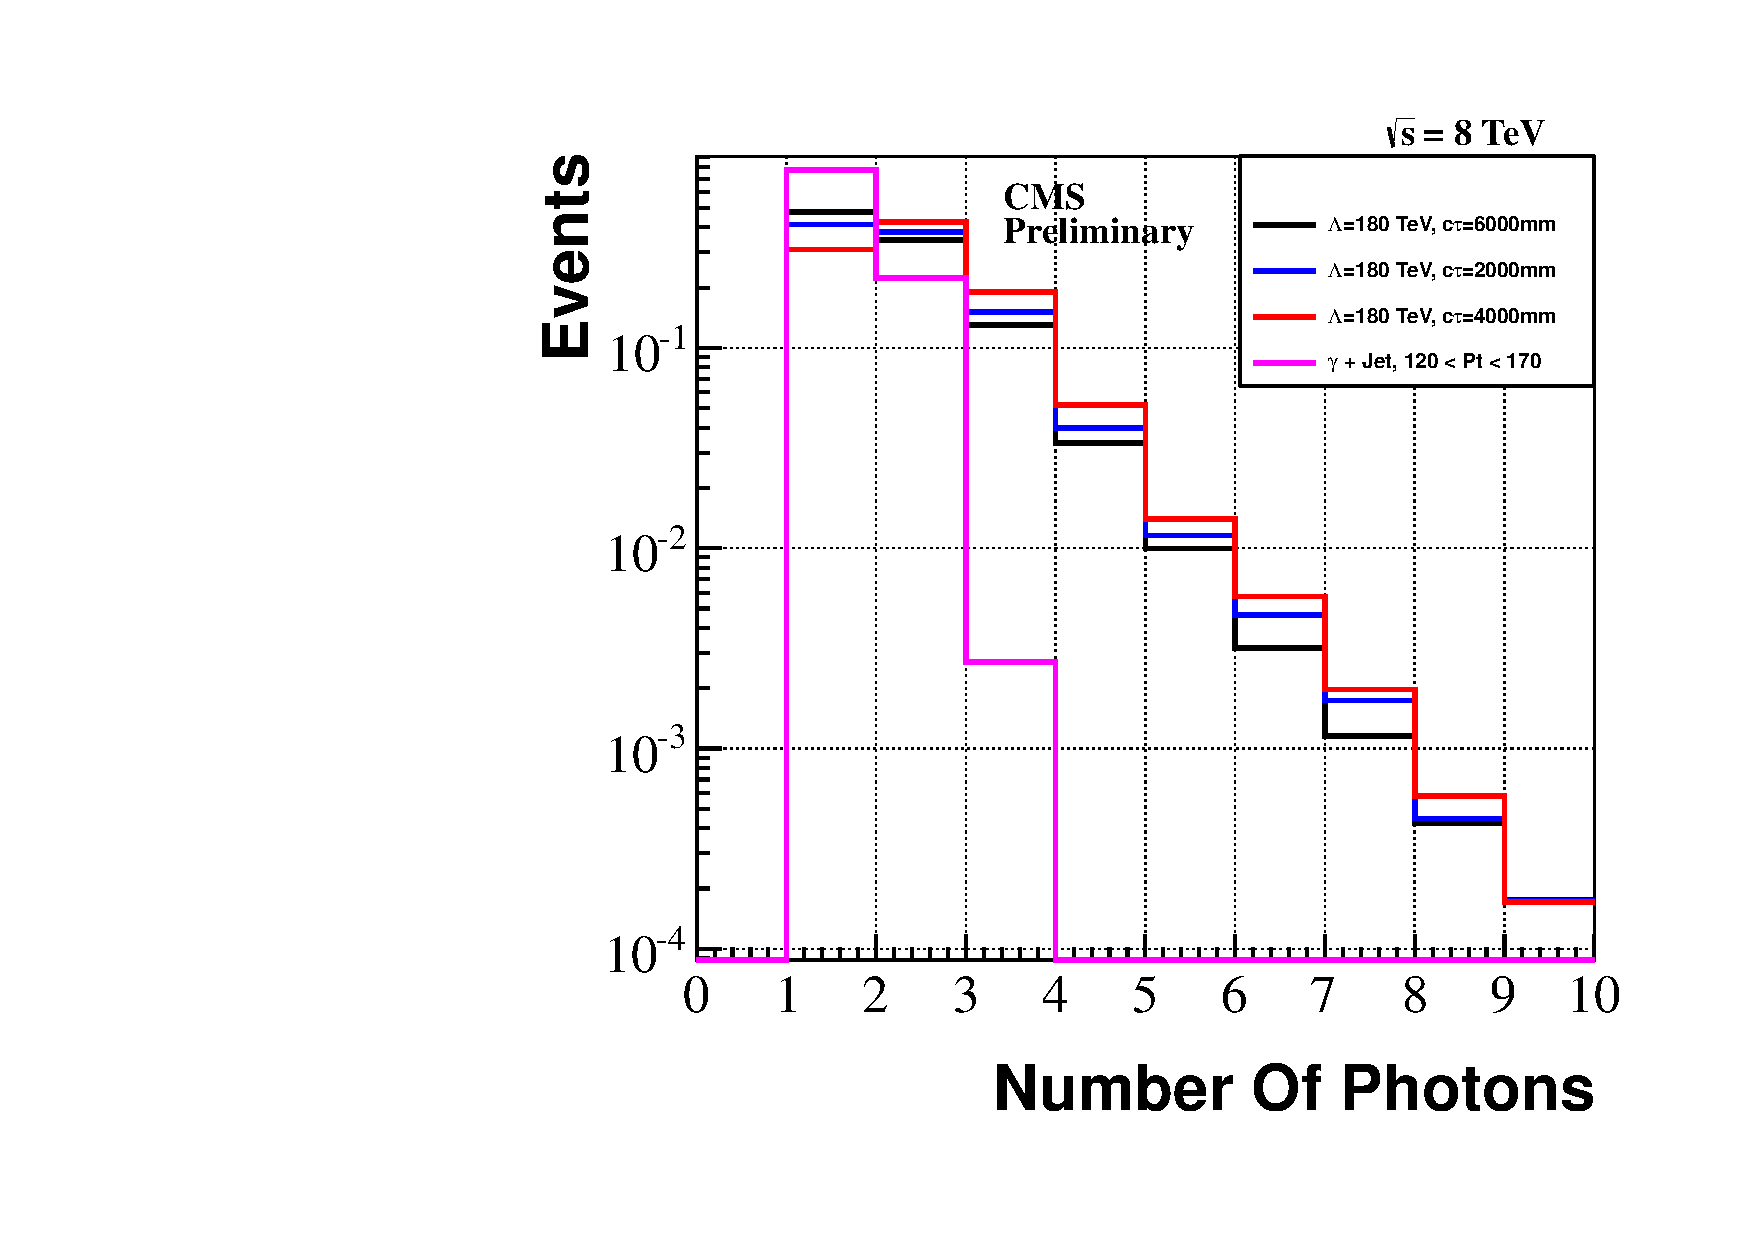
\includegraphics[height=0.5\textwidth,width=0.5\textwidth]{THESISPLOTS/GMSB-SPS8-MODEL-NumberOfPhotons_Lambda-180-TeV.pdf}% \hspace{-1cm}
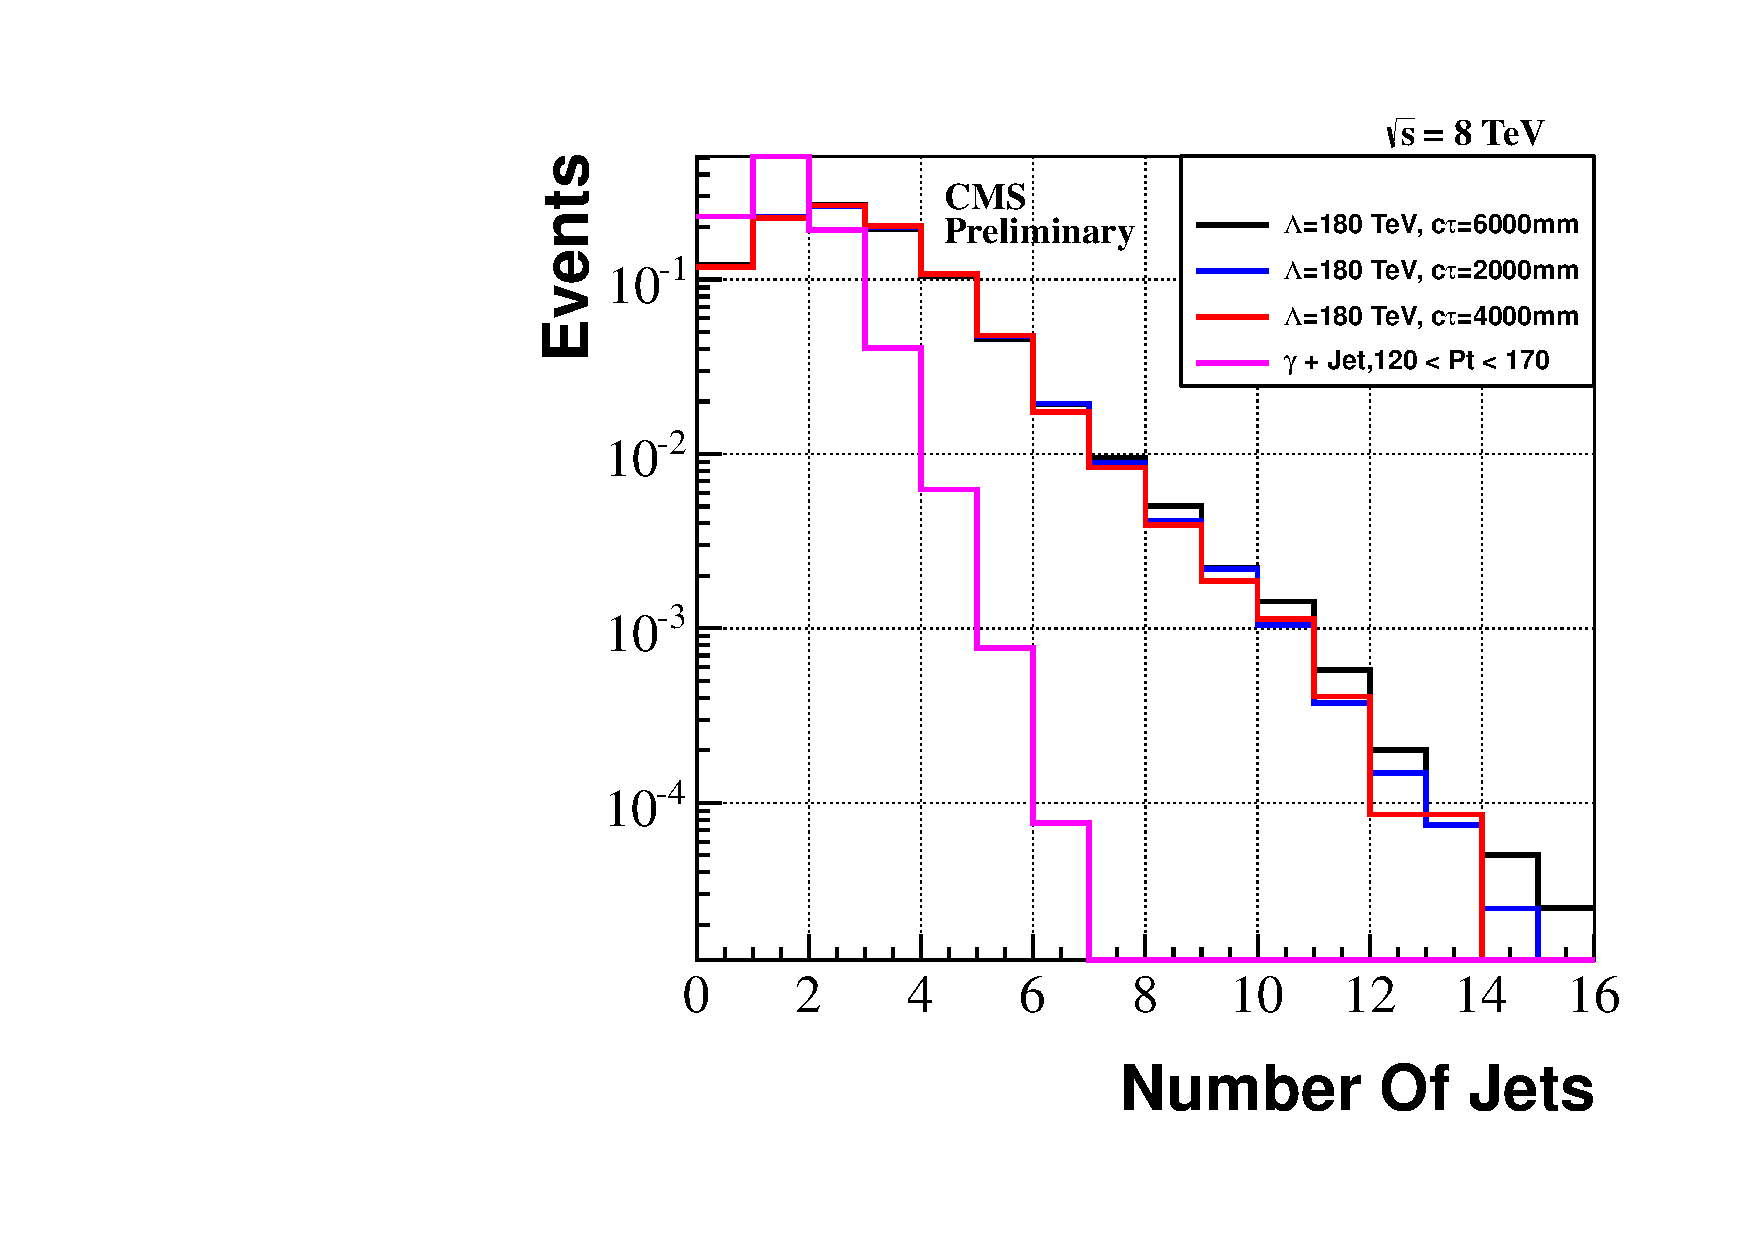
\includegraphics[height=0.5\textwidth,width=0.5\textwidth]{THESISPLOTS/GMSB-SPS8-MODEL-NumberOfJets_Lambda-180-TeV.pdf}} \\
\hspace{0.5cm}
\mbox{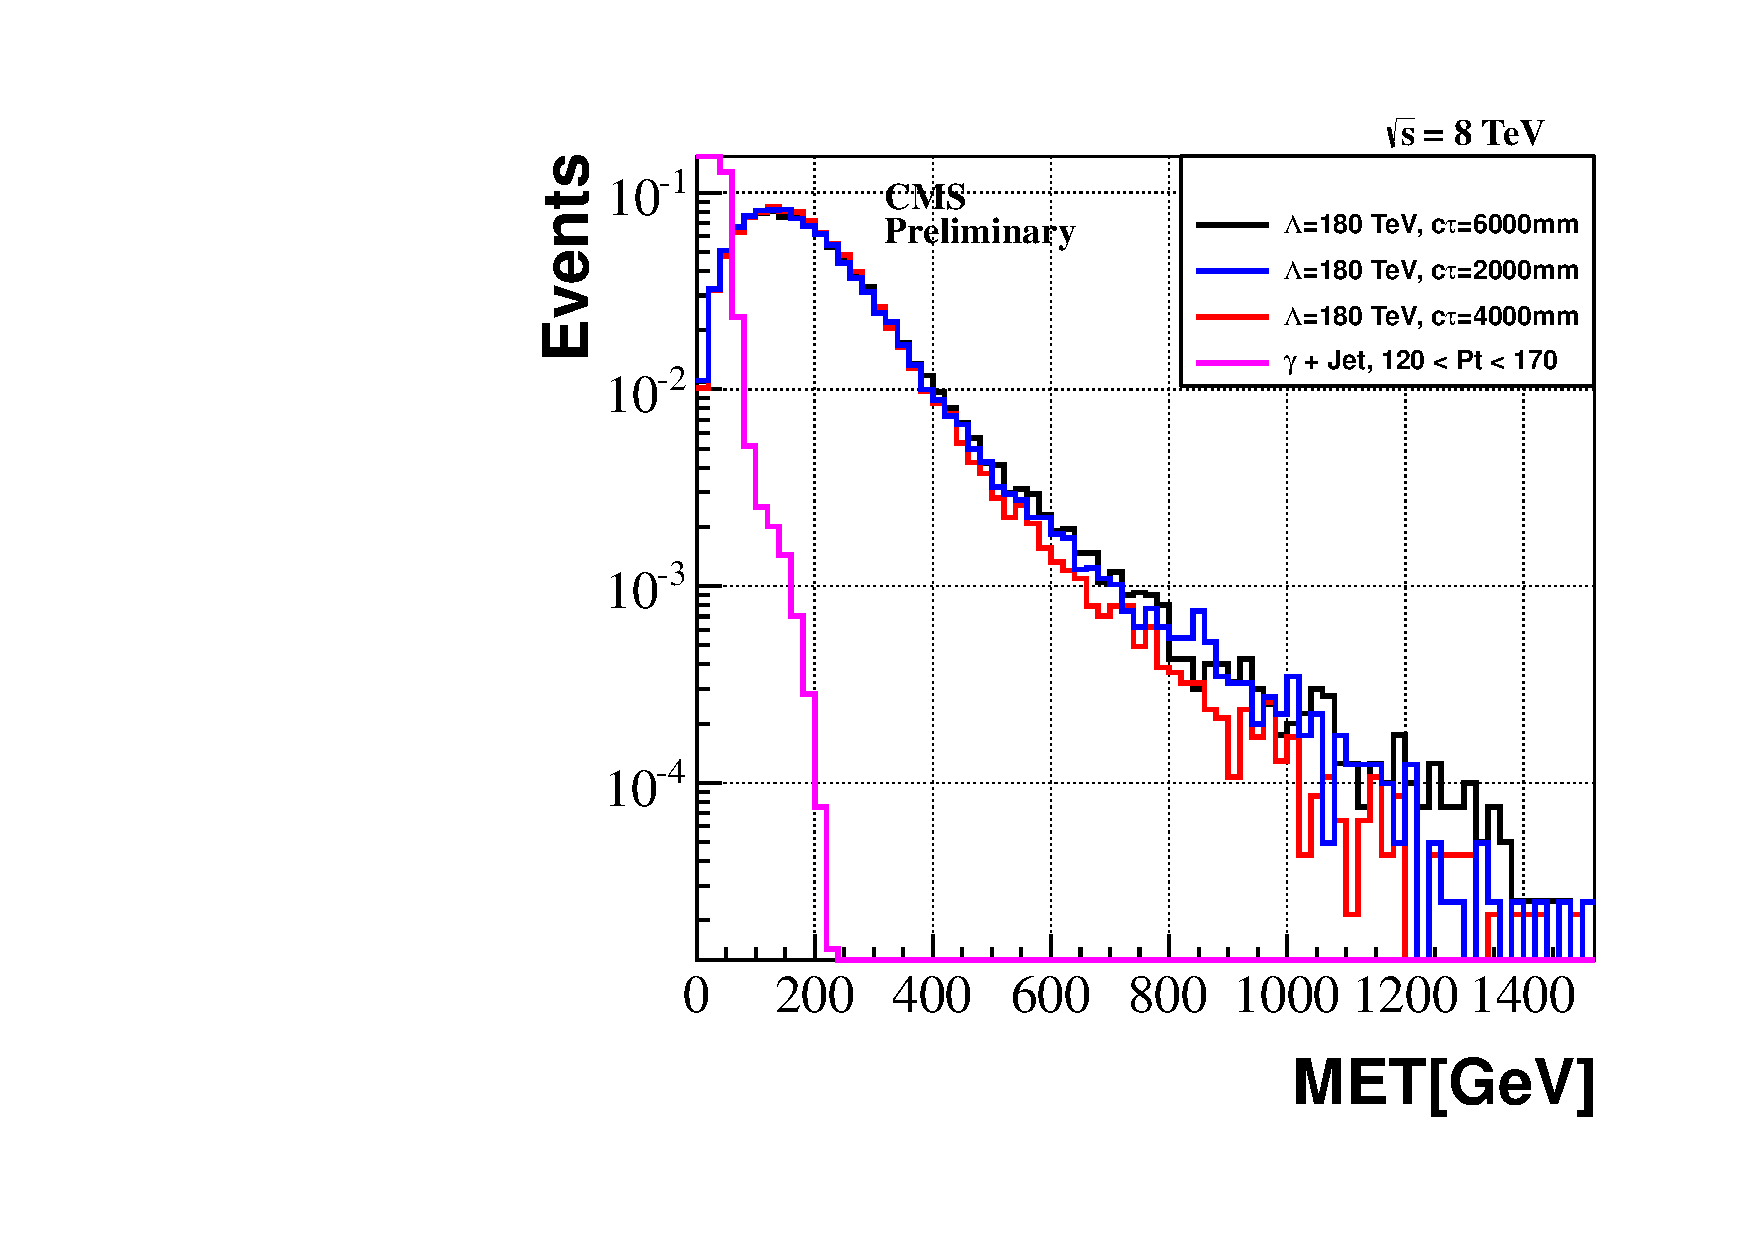
\includegraphics[height=0.5\textwidth,width=0.5\textwidth]{THESISPLOTS/GMSB-SPS8-MODEL-Event-MET_Lambda-180-TeV.pdf}}
\captionof{figure}{Number of photons~(top left),  Number of jets~(top right) and 
\MET~(bottom) for events with \PSneutralinoOne decay to $\gamma$ and $\tilde{G}$ for different $c\tau$ points with $\Lambda=180$\TeV of the SPS8 model. A $\gamma +$jet sample is shown for comparison.}
\label{fig:NKINE}
\end{center}
\end{minipage}
%%%
\subsection{ECAL Time}
The presence of spikes, noisy crystals and pile-up events, demand a robust method for measuring the photon arrival time at  ECAL and since ECAL time is our main observable for distinguishing background from signal events, such a method must reduce timing bias which may arise from such anomalous events. As a result, we studied different methods for measuring the photon arrival time at ECAL. 
\newline
The electromagnetic shower of an electromagnetic particle spreads across several crystals~(energy and time measurements from several channels) which belongs to the particle's supercluster containing all of the particle's energy. Using the supercluster, the arrival time of an electromagnetic particle can be defined either using the reconstructed time~($ t_{reco}$) of a single crystal, which is the crystal with the highest energy deposit~(\textit{seed crystal}), or a weighted average time calculated using the reconstructed time of every crystal of the supercluster. We write $t_{seed}$ for the seed time and $t_{Ave}$ for the average time defined as
\begin{equation}{\label{eq:AVETIME}}
t_{Ave} = \frac{\sum_{i=1}^N\frac{t_{reco, i}}{\sigma_{i}^{2}}}{\sum_{i=1}^{N}\frac{1}{\sigma_{i}^{2}}},
\end{equation}
where $N$ is the total number of crystals of the supercluster, $t_{reco,i}$  and $\sigma_{i}$ are the time and uncertainty on the reconstructed time of each channel, respectively. 
%Algorithms for extracting and calibrating ECAL crystals using the reconstructed hit~(\textit{rechit}) time have been developed
%and we describe them in detail in the coming sections.
%We use $t_{reco}$ to denote the reconstructed time of each hit or crystal.
%We will denote the calibrated reconstructed time of an electromagnetic object as, $T_{reco}$. 
%Measuring the difference of the ECAL measured time between any two reconstructed objects~(which can be individual crystals or electromagnetic objects) arriving from the same nominal point, which in principle are both expected to have the same time, gives a reliable measurement of the timing resolution of the sub-detector including the crystal-to-crystal synchronization factor.  In ECAL timing, the photon reconstructed time, $t_{reco}$, can be calculated using either of the following methods:
%%\begin{enumerate}
%%\item \textbf{seed time}: The time of the highest energy crystal or hit in the highest energy basic cluster~(about $9$ crystals) of the photon super cluster~(about $25$ crystals). It is denoted 
%%\item \textbf{Average or mean time}: This is the error weighted average time of all the crystals in the photon seed basic cluster.
%%It is denoted as $t_{Ave}$ or $t_{mean}$.
%%\end{enumerate}
%Therefore, the arrival time of a photon or an electromagnetic object, $t_{\gamma}$ or $t_{\Pepm}$, can either be given as $t_{seed}$ or $t_{Ave}$.
Figure \ref{fig:TIME} shows a comparison of a photon time measured as the seed time, $t_{seed}$, and as the average time, $t_{Ave}$. The distributions have been normalized to total number of events.

\vspace{5mm}
\begin{minipage}{0.90\linewidth} 
\begin{center}
\mbox{
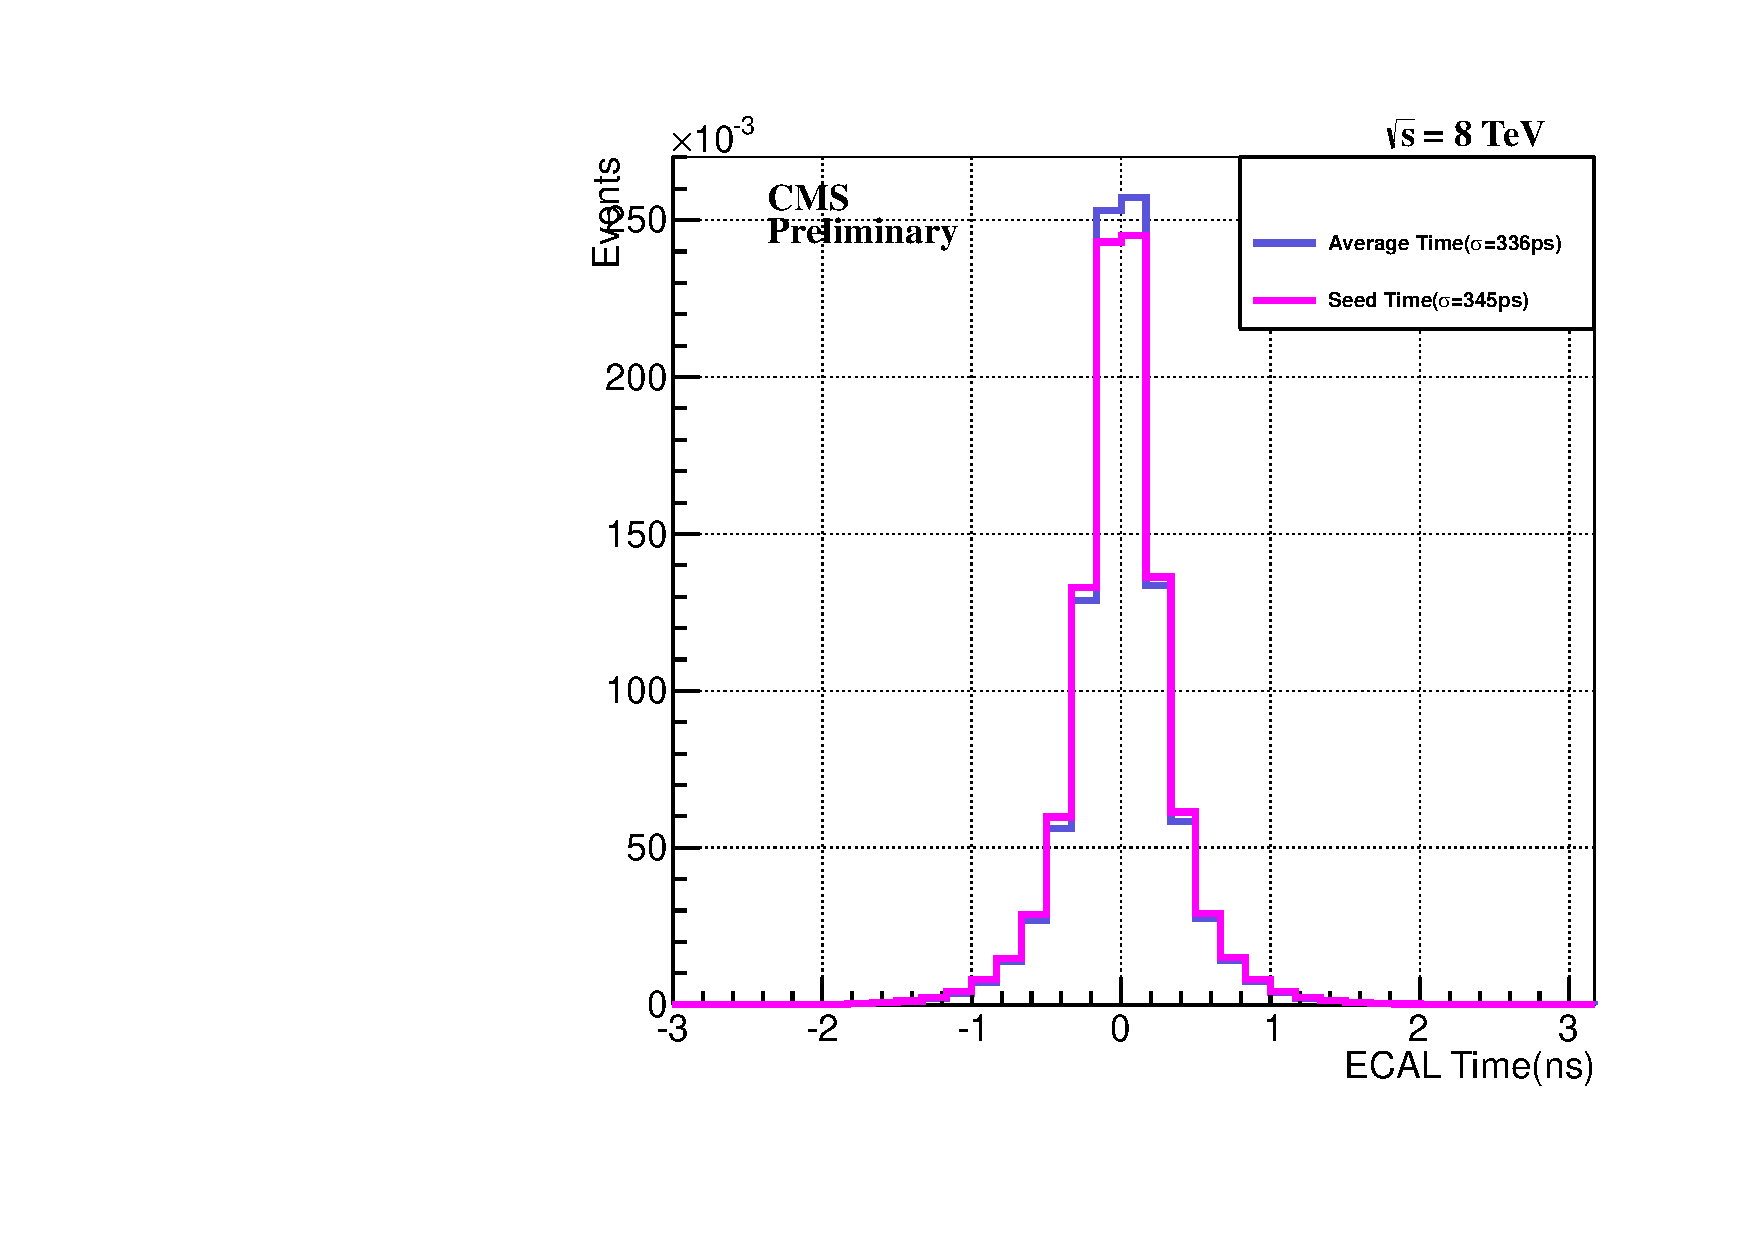
\includegraphics[height=0.50\textwidth, width=0.7\textwidth]{THESISPLOTS/ECAL-SeedVsAveTime-Zee.pdf}
%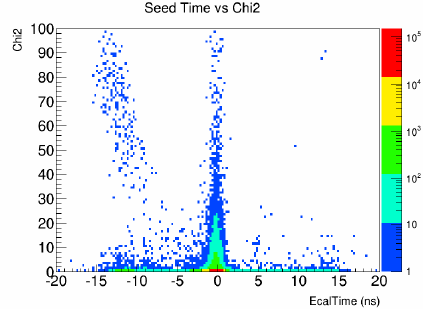
\includegraphics[height=6cm, width=0.5\textwidth]{THESISPLOTS/Seed-Time-Chi2.png}
}
\captionof{figure}{Measuring the photon time using either seed time~(black) or average time~(blue). $\sigma$ of the Gaussian fit from seed time slightly better average time which is computationally intensive.}
\label{fig:TIME}
\end{center}
\end{minipage}

\vspace{5mm}
The spread of both time distributions, $\sigma$ of a Gaussian fit, are very similar. A value of  $\sigma = 345$~ps is observed for seed time compared to $\sigma = 336$~ps for the average time distributions. We used the seed time approach for the photon ECAL time since there is not much to gain from either methods.  \newline
In cases where one or more of the crystals is poorly time calibrated, the photon time from the weighted average time approach is biased. A possible solution for this is to select only properly time calibrated crystals of the supercluster for computing the average time or simply used the times from crystals of the \textit{seed basic cluster}. A supercluster is said to consist of many smaller clusters called \textit{basic clusters}, and the average time of the cluster with the highest energy~(seed basic cluster) can also be used as the particle's measured arrival time.
\paragraph*{}
  A $\chi^{2}$ calculated from the time of all the crystals belonging to the photon supercluster is a useful quantity to legitimized a photon time and we use it to distinguish fake photons~(jets misidentified as photons) and especially spikes from true photons. Figure  \ref{fig:spikeVsPhoton} shows the profile of the pulse shape~(left) of an identified spike with that of a true photon event. A distribution of the normalized $\chi^{2}$ against the ECAL time is shown in the right plot of the same figure. Photons with a signal pulse shape profile as that of spikes are associated with large values of $\chi^{2}$ and usually have earlier ECAl arrival time.
 
 \vspace{5mm}
%\paragraph*{}\mbox{}\\ 
\begin{minipage}{0.90\linewidth} 
\begin{center}
\mbox{
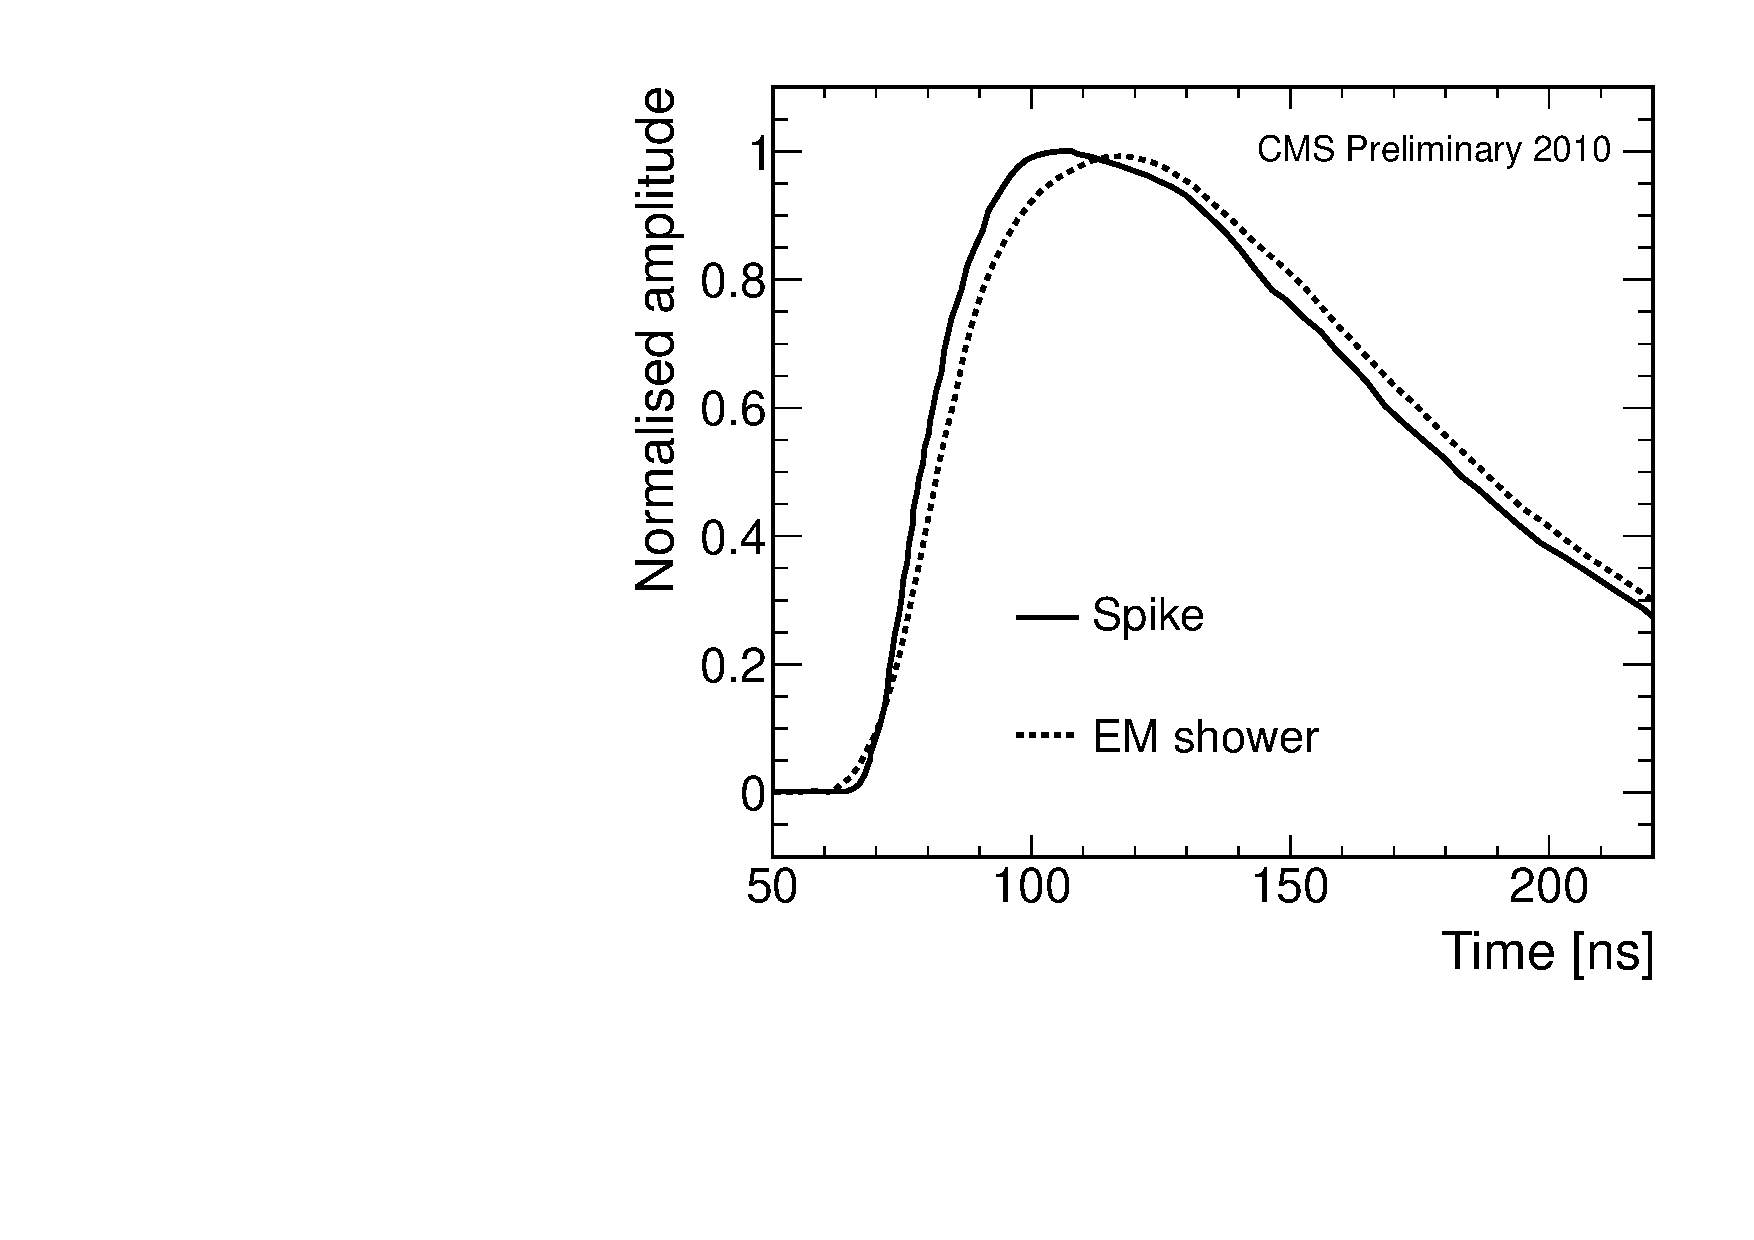
\includegraphics[height=.450\textwidth, width=0.45\textwidth]{THESISPLOTS/spike_pulse_shape.pdf}
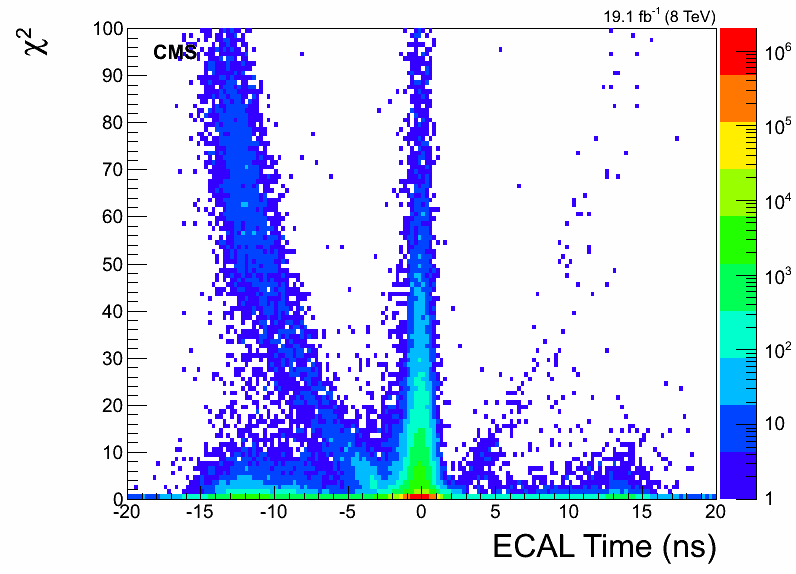
\includegraphics[height=.450\textwidth, width=0.5\textwidth]{THESISPLOTS/seedTime_Chi2.png} }
\captionof{figure}{Pulse shape profile(left) showing a spike~(solid line) and a true EM shower~(dashed line) from data. The $\chi^{2}$ against ECAL time  distribution(right) shows spikes misidentified as photons with very large $\chi^{2}$ with earlier arrival time. The region of $\chi^{2} > 4$ is mostly dominated by spikes events.}
\label{fig:spikeVsPhoton}
\end{center}
\end{minipage}

 \vspace{5mm}
The plot of $\chi^{2}$ against ECAL time~(left plot of Figure \ref{fig:spikeVsPhoton}) shows that most of the photons have ECAL time around zero but also many of the photons with large ECAL time  have large normalized $\chi^{2}$ values which is expected where the time measurements by non-seeded crystals is inconsistent with the time measurement of the seed crystal. We observed that, with a cut in $\chi^{2} < 4$, we can reduce with 99.2\% efficiency, photon arrival time contributions from spikes and misidentified photon events.
%%%
%%%%
\subsubsection*{Simulated ECAL Time}
The ECAL time for late arriving photons which might arise from either the decay of long-lived neutral particles, spikes and noisy crystal channels common during data taking is challenging to properly simulate in MC events. This usually leads to disagreements between ECAL time in data and MC events.
We adjust the time of MC events to account for any data and MC time measurement difference using mostly in-time events~(events with photon time within a $[-2, 2 ]$~ns window).
Selecting in-time events with only one or two jets in data, we find the difference in the peak of the photon time distribution from data with the reconstructed MC time~($t^{MC}_{reco}$) of photons from the $\gamma +$ jets samples. The measured time difference of the average time for reconstructed photons from data and MC $\gamma +$ jet sample, is used to smear the reconstructed MC ECAL time. A average time difference of about $125$~ps is observed between the data and MC ECAL time. After the smearing, both data and MC ECAL time show a close agreement for the photon arrival time. The photon ECAL time from data and MC $\gamma +$ jet sample both shown in Figure \ref{fig:DATAMCTime} comparing before~(left plot) and after~(right plot) the adjustment on MC ECAL time was made. 
%We performed the same smearing for all MC samples used in our analysis.
\newline
 It is worth noting that the difference of 125~ps between $t^{MC}_{reco}$ and $t^{DATA}_{reco}$ compared to 500~ps ECAL timing resolution is not enough to enormously impact our event selection. %however, simulating photons ECAL time in the tails of the time distribution still remains.

\vspace{5mm}
%\paragraph*{}\mbox{}\\
\begin{minipage}{0.90\linewidth} 
\begin{center}
\centering
\mbox{
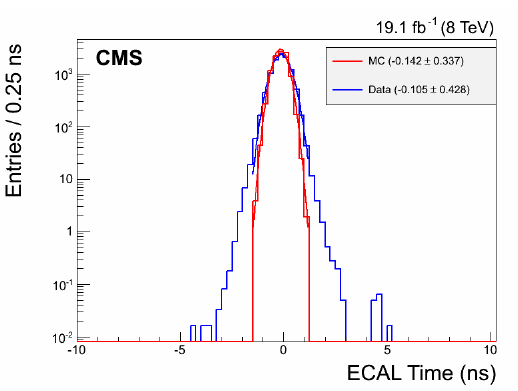
\includegraphics[height=0.5\textwidth, width=0.5\textwidth]{THESISPLOTS/MC_Vs_DataTimeB4Calib.png}
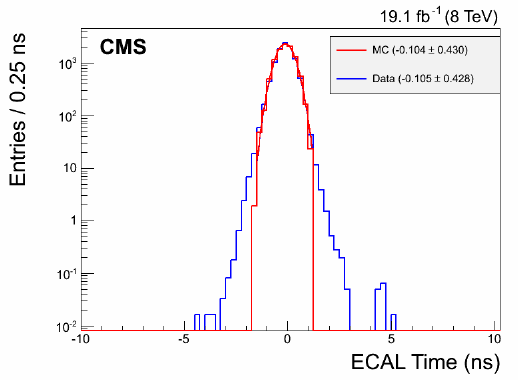
\includegraphics[height=0.5\textwidth, width=0.5\textwidth]{THESISPLOTS/MC_Vs_DataTimeAferCalib.png}
}
\captionof{figure}{ECAL time distributions of in-time photons from MC $\gamma +$ jets~(blue)  and data~(red) samples before~(left) and after~(right) we adjusted the photon time from MC.}
\label{fig:DATAMCTime}
\end{center}
\end{minipage}
%%%
\clearpage
\subsubsection{Neutralino Measured Lifetime}
The distance traveled in the transverse~($x-y$) plane in the CMS detector by the \PSneutralinoOne before it decays, mentioned previously in the subsection \ref{NeutralinoDecay}, is given as
\begin{equation}{\label{eq:decaylength}}
\mathrm{L} = \left(c\tau_{\PSneutralinoOne}\right) \cdot \left( \gamma \beta_{T}\right) = \left(c\tau_{\PSneutralinoOne}\right) \cdot \left( \frac{\pt}{m_{\PSneutralinoOne}}\right).
\end{equation} 
The \pt and mean lifetime~($c\tau_{\PSneutralinoOne}$) of the \PSneutralinoOne determines this distance. Large values of $c\tau_{\PSneutralinoOne}$ means, this distance is large extending even beyond the ECAL volume where detecting the \PSneutralinoOne is not possible while small values of $c\tau_{\PSneutralinoOne}$ means the \PSneutralinoOne decayed quite early and the photon ECAL arrival time is not large enough and detection using ECAL time measurements only is not very reliable. High \pt also means the \PSneutralinoOne is very boosted and can also travel out of the ECAL before it decays while low \pt means the \PSneutralinoOne is less boosted and traveling slow enough for the photon to be delayed at ECAL. In Figure \ref{fig:NKINE}, we show  distributions of the \pt of the \PSneutralinoOne~($\pt^{\PSneutralinoOne}$), its transverse distance traveled, transverse momentum of the photon~($\pt^{\Pphoton}$) and photon's estimated arrival time~($T_{\Pphoton}$)  at event generation level. These distributions are for different $\mathbf{\Lambda}$ and $c\tau_{\PSneutralinoOne}$ points of the SPS8 model. We observed that, the \pt of the \PSneutralinoOne increases with increase values of $\Lambda$, from $\Lambda = 100$ to 300\TeV,  which agrees with our expectation in that, increasing values of $\Lambda$ implies increasing values for the gluino/squark masses which cascade decay to the \PSneutralinoOne. In the same way, increasing values for $\Lambda$ means the \PSneutralinoOne becomes more massive and hence the photon \pt also increases. For a fixed value of $\Lambda$ \ie \pt of the nuetralino is the same, the transverse distance traveled by the \PSneutralinoOne before decay~(top right plot of Figure \ref{fig:NKINE}) and photon expected time at ECAL(bottom right plot of Figure \ref{fig:NKINE}) increased with increased value of \PSneutralinoOne lifetime, $c\tau = 250$ to $6000$\mm. The qualitative agreement of the distributions of both plots confirms our expectation that the photon is delayed as a result of the long lifetime of the \PSneutralinoOne. However, one can argue that this is not entirely the case as we study in detail the source of delayed photons in the next section.

\vspace{5mm}
\begin{minipage}{0.95\linewidth} 
\begin{center}
\mbox{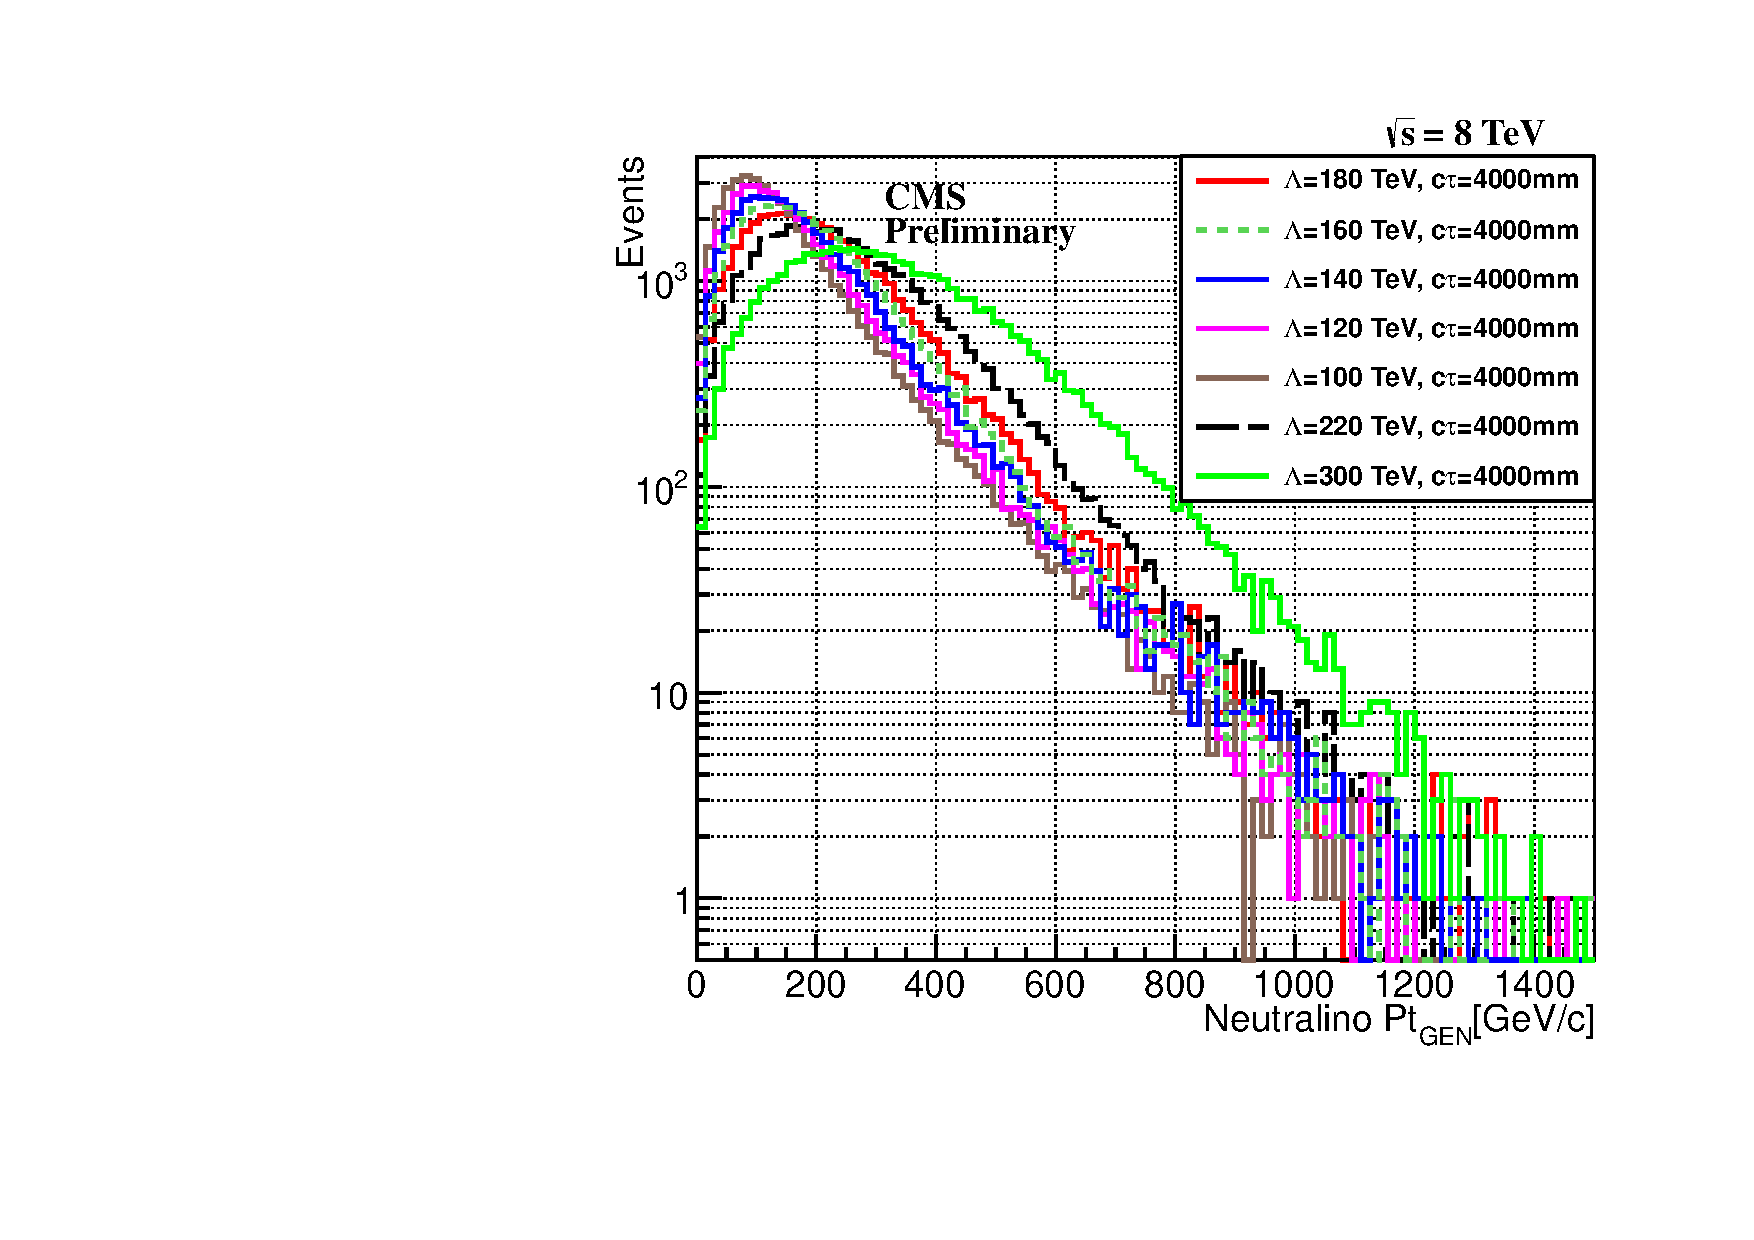
\includegraphics[height=0.45\textwidth,width=0.5\textwidth]{THESISPLOTS/GMSB-SPS8-MODEL-Neutralinio-Pt_ctau-4000-mm.pdf} %\hspace{-1cm}
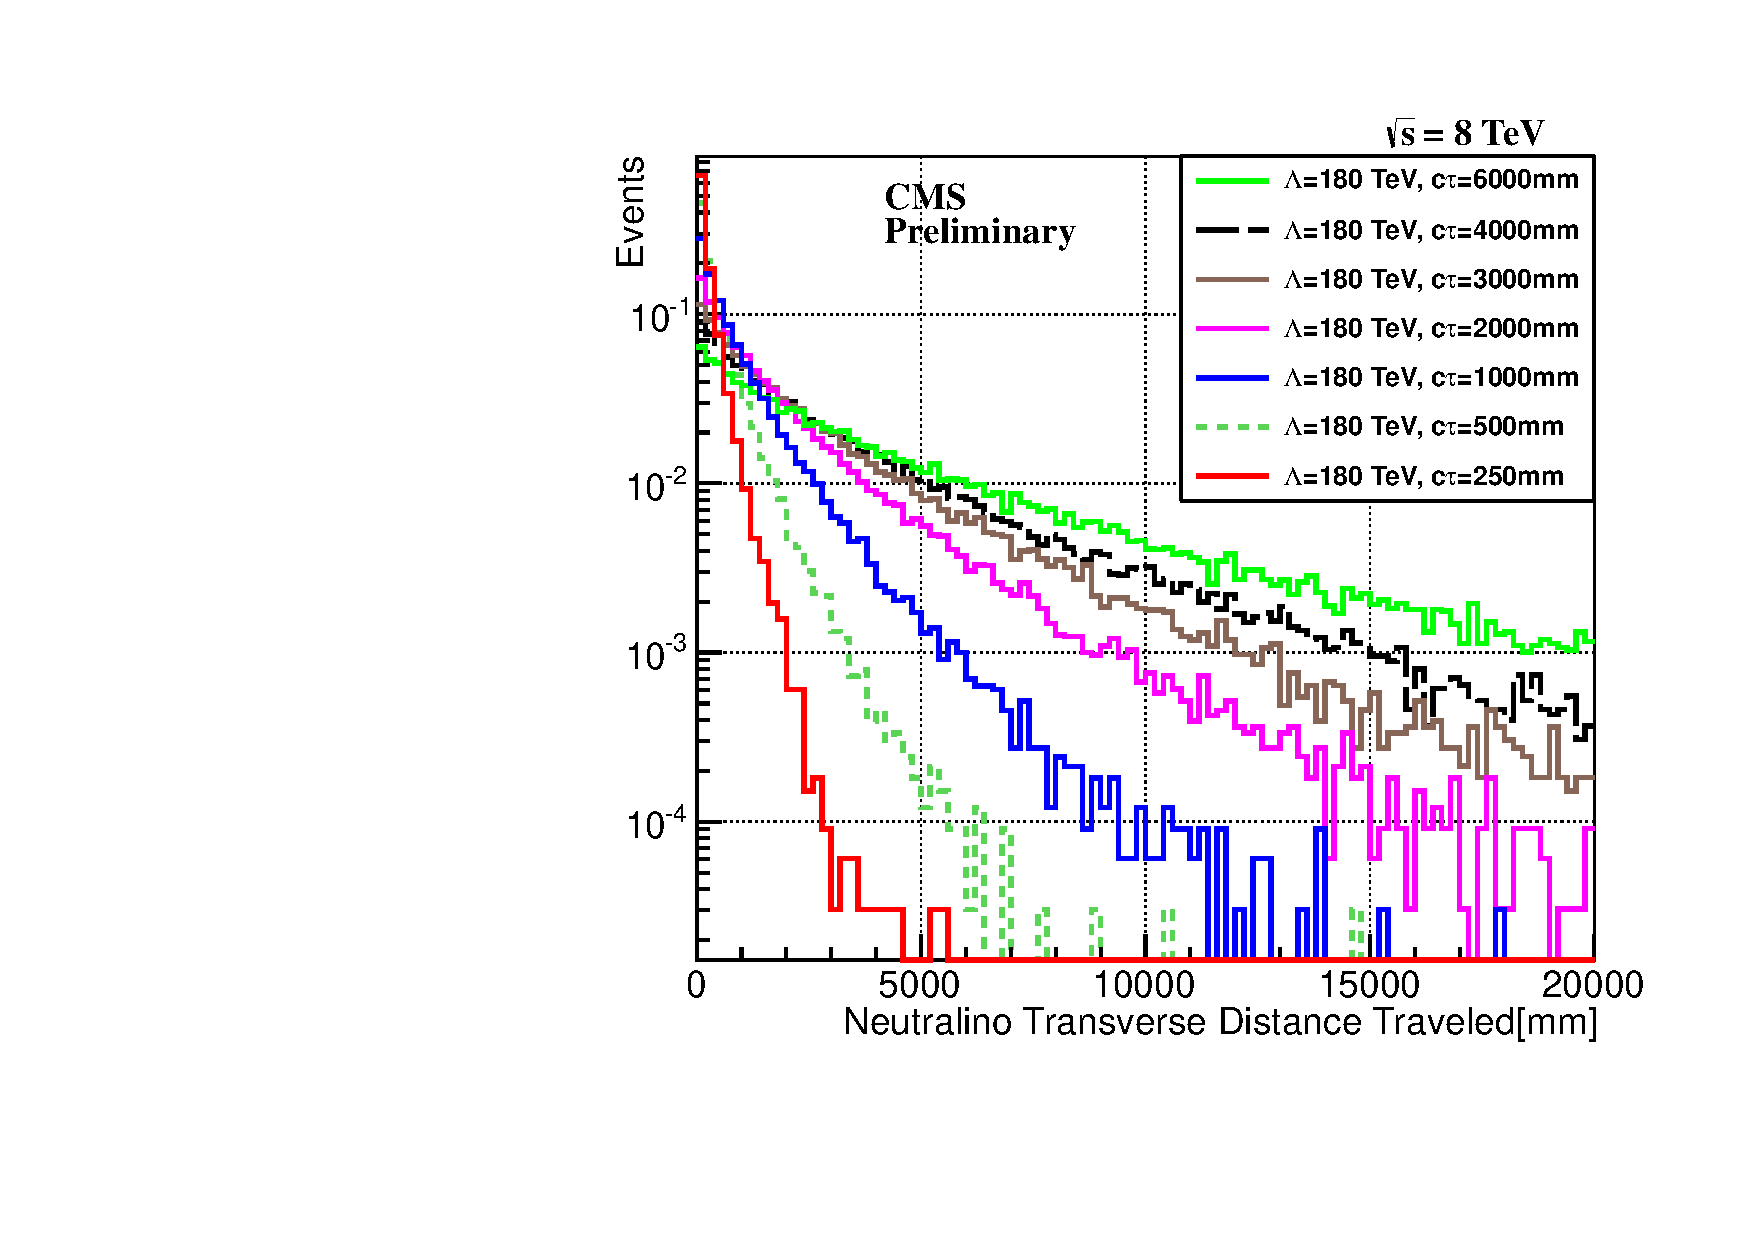
\includegraphics[height=0.45\textwidth,width=0.5\textwidth]{THESISPLOTS/GMSB-SPS8-MODEL-Neutralino-Proper-DecayLength_Lambda-180-TeV.pdf}} \\
\hspace{0.5cm}
\mbox{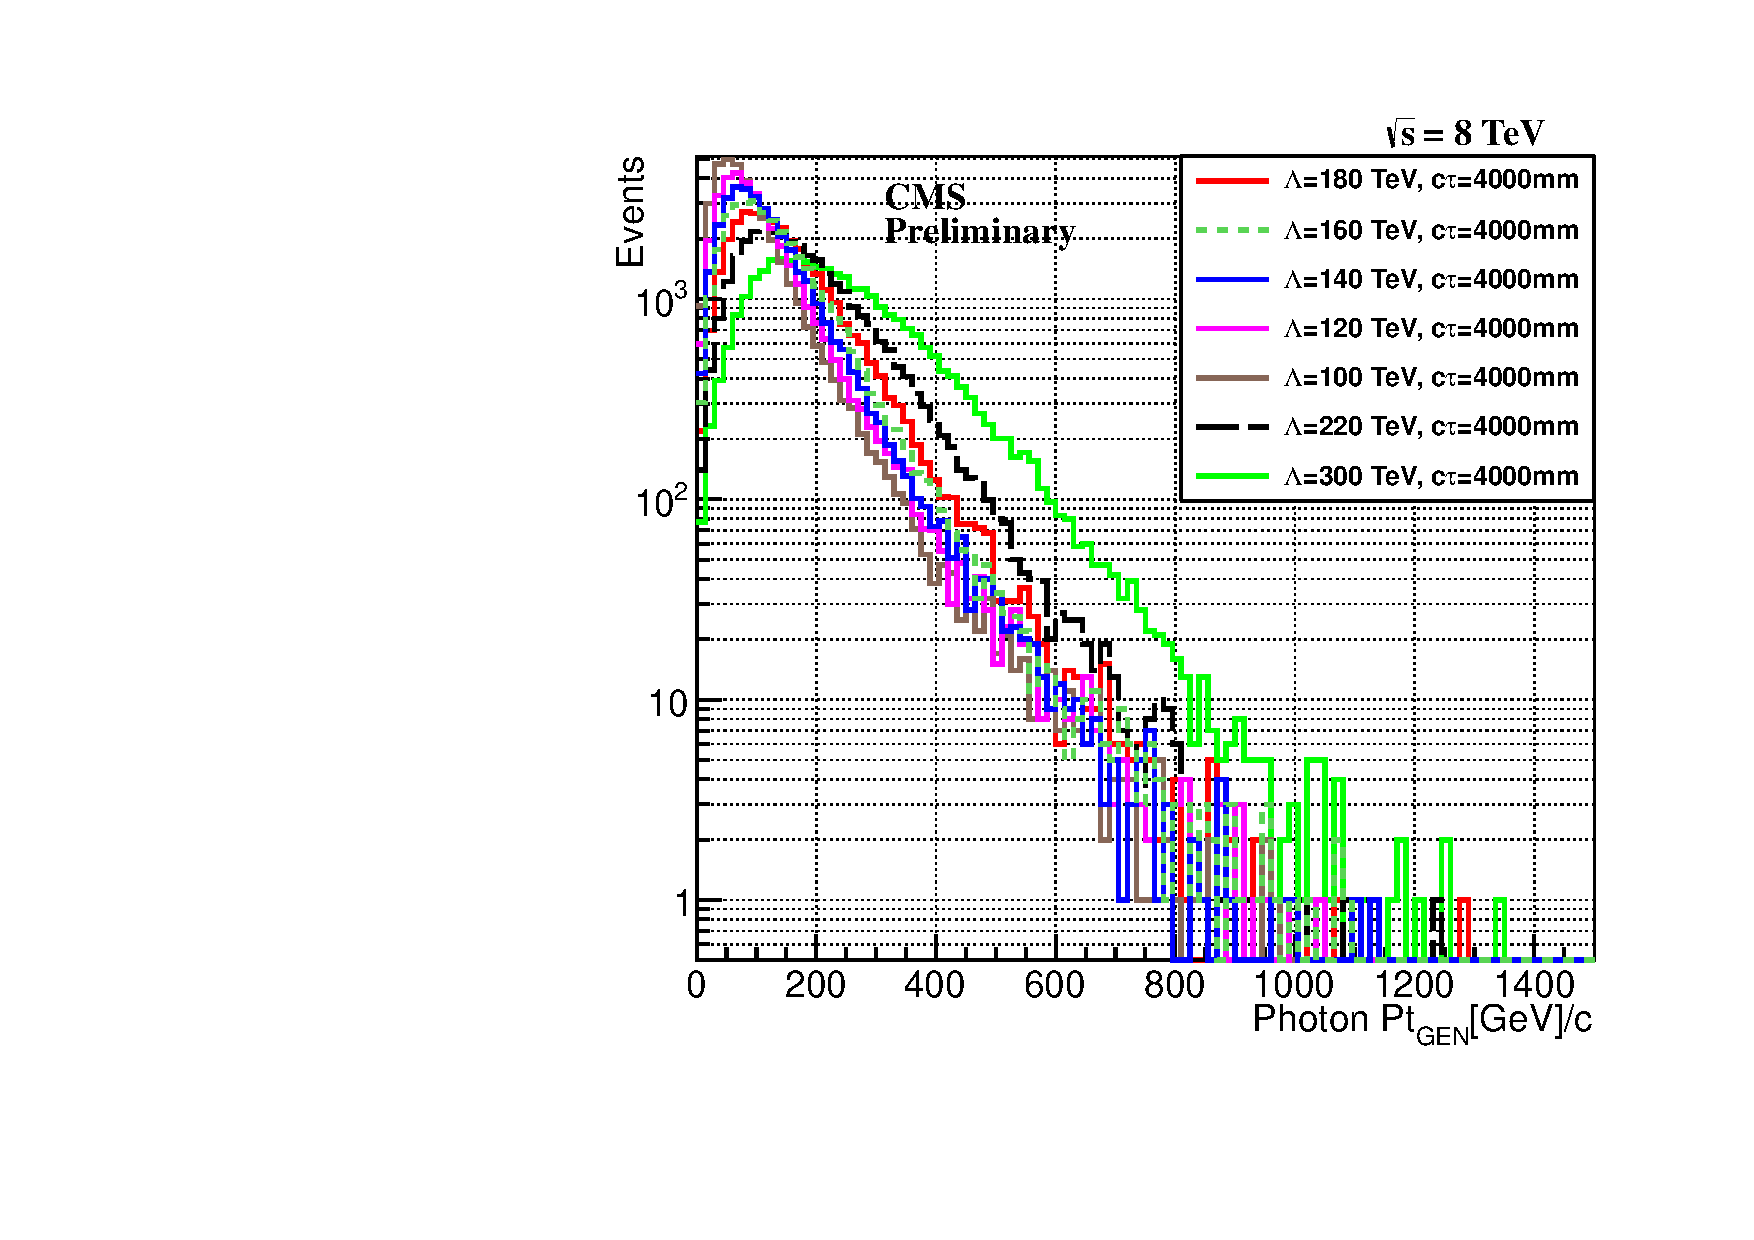
\includegraphics[height=0.45\textwidth,width=0.5\textwidth]{THESISPLOTS/GMSB-SPS8-MODEL-Photon-Pt_ctau-4000-mm.pdf} %\hspace{-1cm}
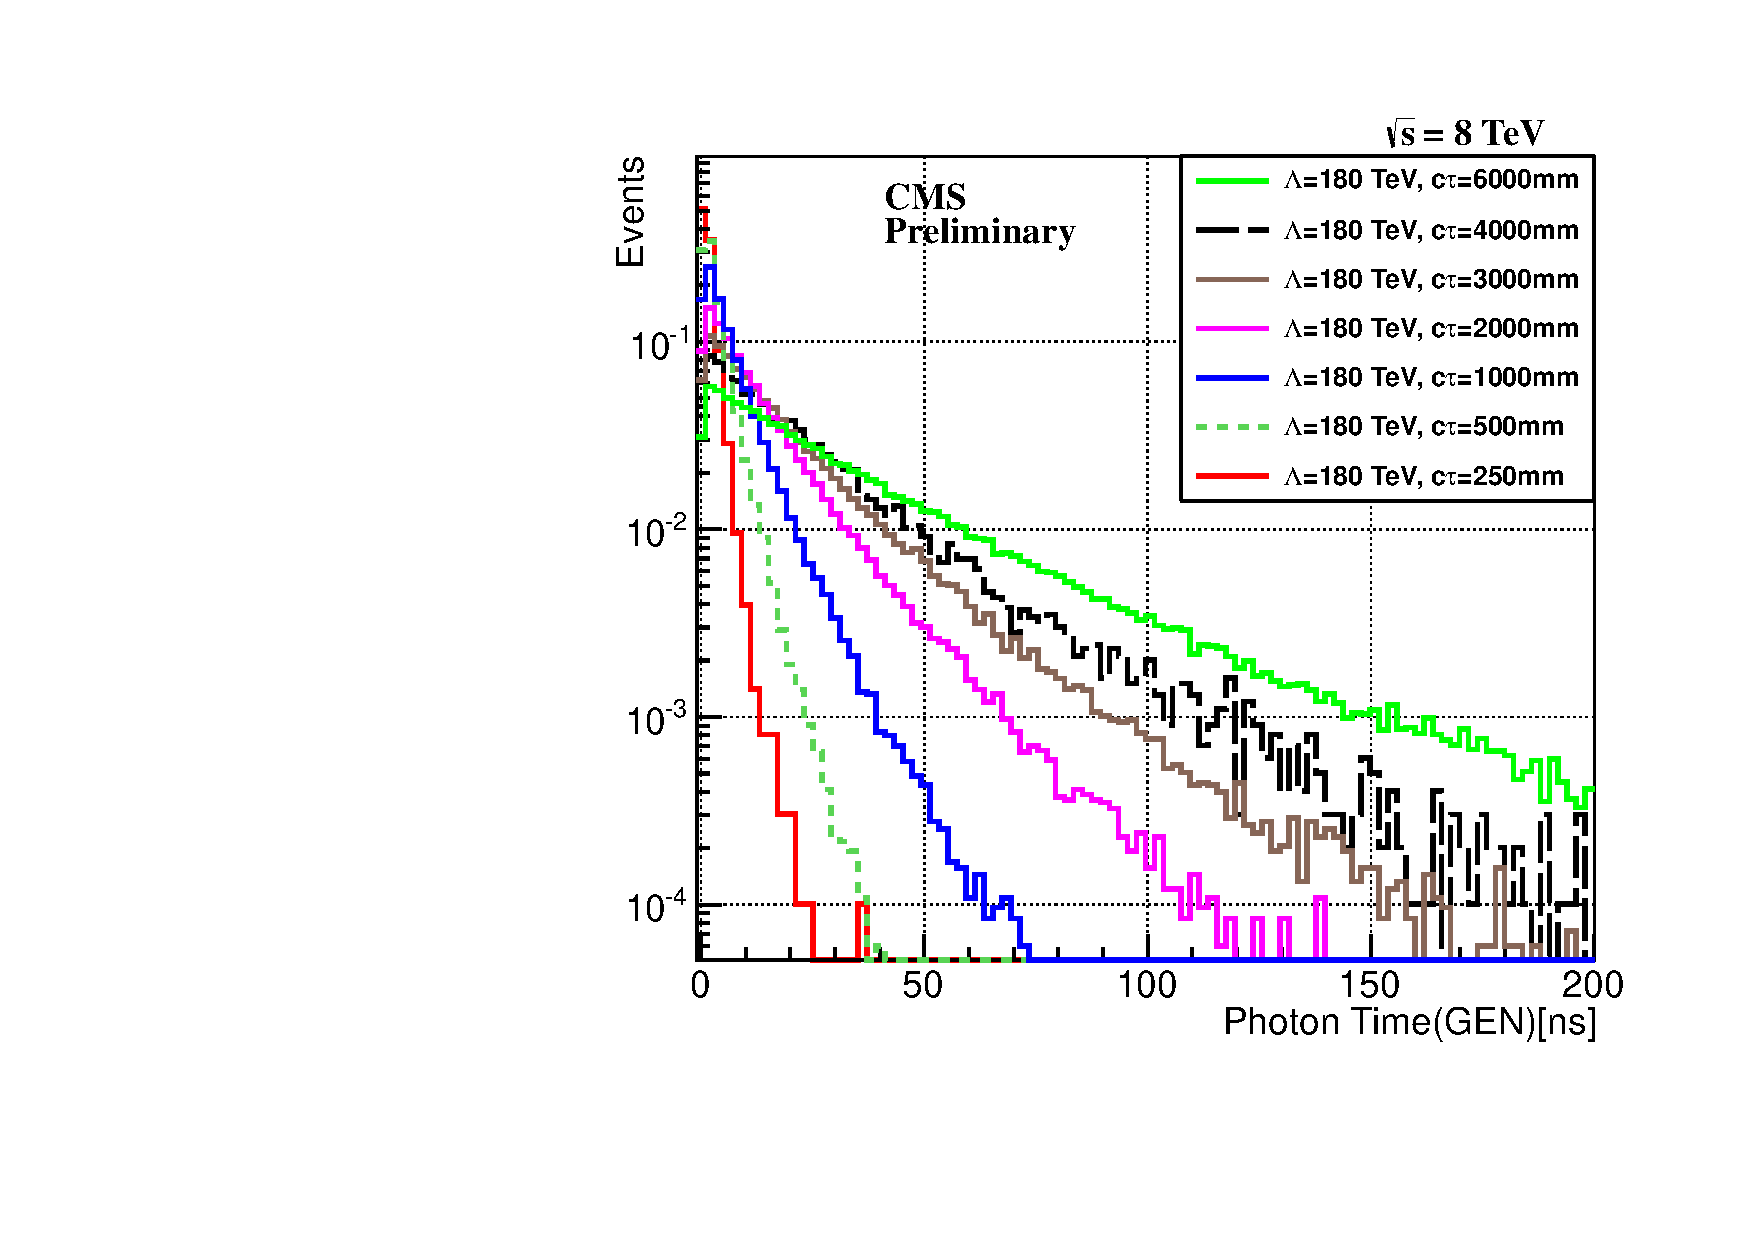
\includegraphics[height=0.45\textwidth,width=0.5\textwidth]{THESISPLOTS/GMSB-SPS8-MODEL-Photon-GEN-Time_Lambda-180-TeV.pdf}}
\captionof{figure}{Neutralino transverse momentum distribution~(top left) and transverse distance traveled~(top right). Transverse momentum~(bottom left) and time~(bottom right) of photon from neutralino decay for different $\Lambda$ and $c\tau$ points in GMSB SPS8 model.}
\label{fig:NKINE}
\end{center}
\end{minipage}
 
\subsubsection*{Source of Delayed Photons}
The photon from the decay of \PSneutralinoOne can arrive late at ECAL for either one of the following reasons: because the \PSneutralinoOne is traveling slow \ie with $\beta=\frac{p_{\PSneutralinoOne}}{m_{\PSneutralinoOne}} << 1$, or because the \PSneutralinoOne was produced with significant boost such that the photon traveled to ECAL through a non-direct flight path from the nominal $pp$ interaction point. We distinguish between these two sources of delayed photons from an estimate of the photon arrival time at ECAL using the  distance traveled by \PSneutralinoOne before decay and photon distance travel from decay point to the point of detection at ECAL. Figure \ref{fig:DELAY}(left) is a schematic diagram showing how we estimate the photon arrival time at ECAL in each of the possible different travel flight path representing the different source of delayed photons. The estimated photon arrival ECAL time for each scenario is given as follows:
\begin{itemize}
  \item From slow moving neutralinos: $\Delta t_1$ = (L1/c$\beta$) - (L1/c)
  \item From non-direct traveled flight path: $\Delta t_2$ = (L1 + L2 - L3)/c
  \item ECAL measured time = $\Delta t_{1} + \Delta t_{2}$
\end{itemize}
%\newline
\begin{minipage}{0.90\linewidth} 
\begin{center}
\mbox{
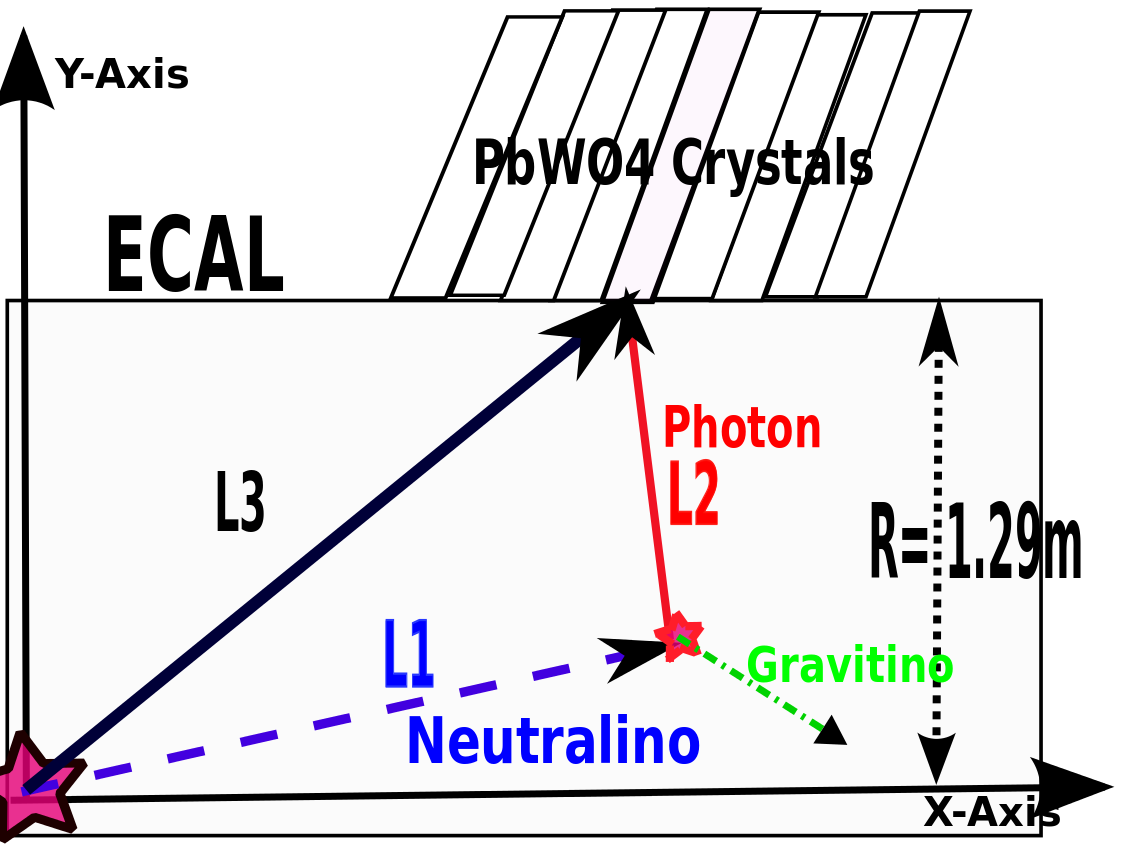
\includegraphics[height=0.55\textwidth, width=0.5\textwidth]{THESISPLOTS/DelayedPhoton-ECAL.png}
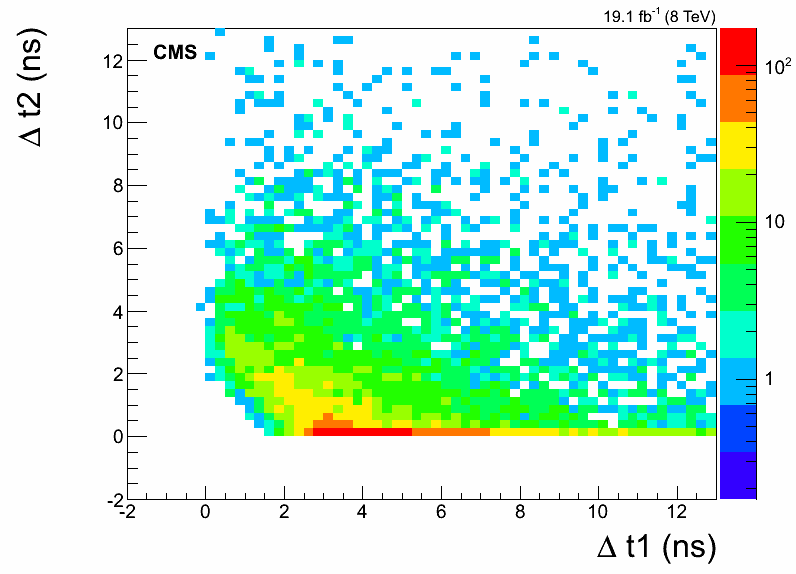
\includegraphics[height=0.55\textwidth, width=0.5\textwidth]{THESISPLOTS/dt1_dt2_late.png}
}
\captionof{figure}{Schematic diagram showing $\tilde{\chi}^{0}_{1} \rightarrow \gamma + \tilde{G}$ decay topology within the ECAL volume of the CMS detector~(Left). Estimated photon arrival time at ECAL  from the decay of neutralinos in the SPS8 model with $m_{\PSneutralinoOne}=256$\GeVcc and $c\tau = 6$\m~(Right).}
\label{fig:DELAY}
\end{center}
\end{minipage}

\vspace{5mm}
The \PSneutralinoOne is traveling with velocity $v = c\beta$, where $c$ is the speed of light in vacuum. The distribution of the estimated photon ECAL arrival times $\Delta t_{1}$ and $\Delta t_{2}$, plotted as shown in Figure \ref{fig:DELAY}(right), where the color intensity represents the photon population, shows that most of the late arrival time photons are from the decay of slow moving neutralinos  compared to those arriving late because of their non-direct flight path to ECAL. This proves that a good number of neutralinos produced with low \pt such that the ratio $\frac{\pt}{m_{\tilde{\chi}^{o}_{1}}} << 1$ are very detectable using ECAL time measurements while those with very long lifetimes produced with high \pt will very likely escape the ECAL without detection unless their decay happen within the ECAL volume such that the delayed photon arrives ECAL through a non-direct flight path.
%%%%%
\subsubsection*{Satellite Bunch Time}
We observed~(see Figure \ref{fig:TIMEECAL}) a 2.5~ns discrete pattern in the reconstructed photon arrival time for events, produced in $pp$ collisions, with the photon arriving in the barrel and endcap regions, \ie $|\eta_{\gamma}| < 3.0$, of the ECAL detector and satisfying a photon transverse momentum requirement of $\pt > 50$\GeVc.

\begin{minipage}{0.90\linewidth} 
\begin{center}
\centering
\mbox{
%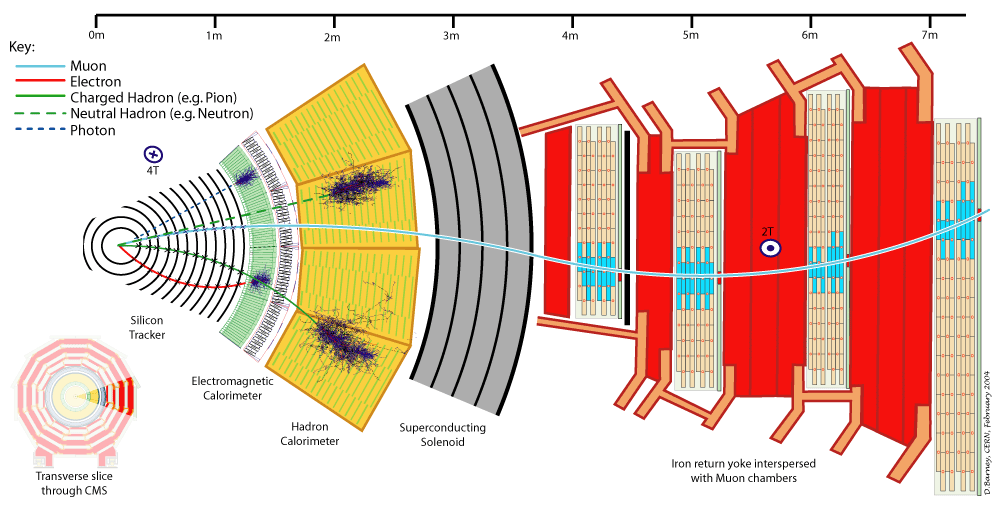
\includegraphics[scale=0.2]{THESISPLOTS/CMS_Slice.png}
%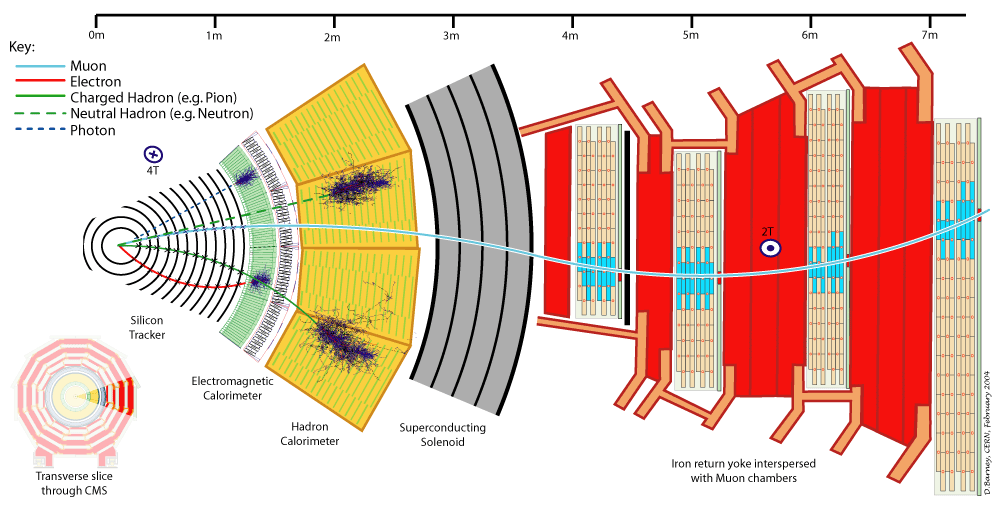
\includegraphics[scale=0.2]{THESISPLOTS/CMS_Slice.png}
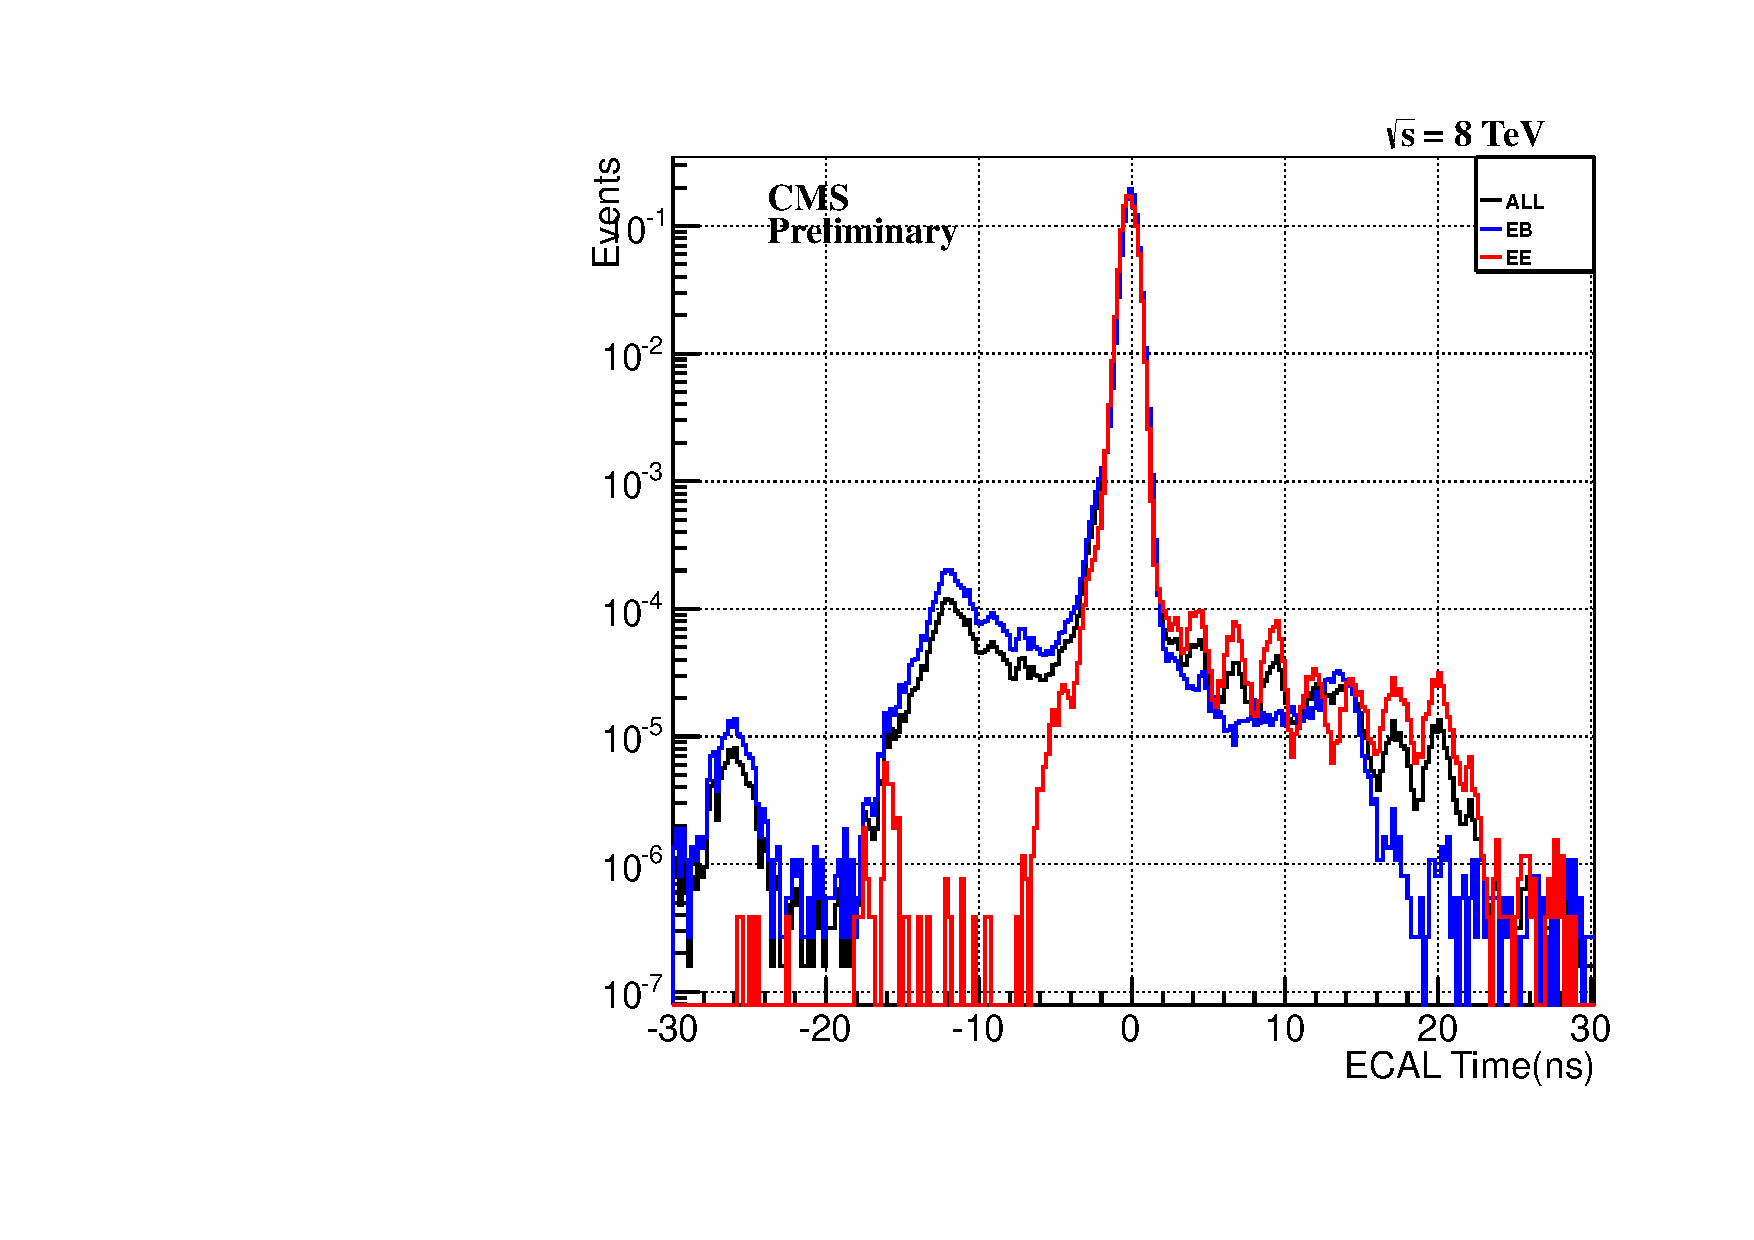
\includegraphics[height=0.65\textwidth, width=0.9\textwidth]{THESISPLOTS/Data-Photon-TimeEBEBALL.pdf}
}
\captionof{figure}{ECAL timing distribution of photons in barrel~(\textcolor{blue}{EB}), endcap~(\textcolor{red}{EE}) and all of ECAL~(\textcolor{black}{ALL ECAL}) with $\pt > 50$~GeV from data. A $2.5$~ns delay timing structure is observed in endcaps.}
\label{fig:TIMEECAL}
\end{center}
\end{minipage}

\vspace{5mm}
A majority of the photons with this signature are from the endcap~($1.47 < \eta < 3.0$) and not many are from the barrel~($|\eta| < 1.47$) region. Photons with this signature are produced from the  collisions of protons in \textit{Ghost}/\textit{Satellite} bunches, described in  section \ref{Ghost}, with either the main proton collision bunch or other \textit{Ghost}/\textit{Satellite} bunches. We consider events with such photons as background events from collisions contributing as an irreducible source of background to our late photon signal. It is very challenging to reject or estimate the contribution from these background events quantitatively. However, using the ratio of the proton population from the LHC RF cavity proton filling profile of ghost to main proton bunches, we estimate that one in every $10,000$ photons from $pp$ collisions observed in ECAL is from ghosts bunches, with most of the photons from ghost bunches belonging to the endcap regions. Their limited presence in the barrel is because very few of them are produced with high enough \pt to travel to the barrel region. 
\newline
The observation of this phenomenon along with the sub-par ECAL time resolution in the endcaps compared to the barrel, allows us to accept only  photons in the barrel in this analysis.
\newline
Using events with moderate \pt range electromagnetic particles in the barrel such as events with $\PZ \rightarrow \EE$ decay, we studied and estimated the background events contribution from \textit{Ghost}/\textit{Satellite} proton collisions to the late photon signal. The details of this study and the results obtained is discussed in the collision background estimation section of this chapter.
%%%
\paragraph*{\MET Adjustments} \mbox{}\\
  The official CMS electromagnetic calorimether supercluster reconstruction criteria used in the PF event reconstruction algorithm does not include "out-of-time" energy deposits in ECAL. The purpose is to avoid energy deposits not produced from the main proton-proton bunch collisions like machine induced backgrounds. As a result, the photon \et contribution from events with out-of-time photons is not included in the calculation of the event missing transverse energy or \ETslash\hspace{0.15cm}(from now on, we will be using for convenience, \ETslash\hspace{0.15cm} instead of \MET as the symbol for missing transverse energy). This non-inclusion of the out-of-time photon \et, introduces some difference in the calculation of \ETslash\hspace{0.15cm} between in-time~($|t_{\gamma}| < 3.0$~ns) and out-of-time photon events. 
\newline
In our analysis, energy deposits from events with out-of-time photons belong to possible signal events since we are searching for large arrival time photons. Because the out-of-time photon's transverse energy~(\ET) is not included in the sum total transverse momentum for events with out-of-time photons in calculating the total transverse momentum imbalance, we correct for this by adding the out-of-time photon's $\ET$ vector to the  particle flow reconstructed \ETslash\hspace{0.15cm}~(PF-MET) vector. We introduced an additional missing transverse energy variable defined as $\vec{{\ETslash}^{\gamma}\hspace{0.15cm}} = \vec{\ETslash}\hspace{0.25cm} + \vec{\et}$, in our final event selection to avoid any bias is the event selection, particularly for events with out-of-time photons. 
%%The difference between $\ETslash$\hspace{0.25cm} and ${\ETslash}^{\gamma}$ is given as
%%\begin{enumerate}
%%\item ${\ETslash}$~ : PF-MET equal to $\ETslash$\hspace{0.25cm} from standard event reconstruction.
%%\item ${\ETslash}^{\gamma}$~: PF-MET with photon \ET vector subtracted \ie ${\ETslash}^{\gamma} = \ETslash\quad - ~\et$ of the  out-of-time photon.
%% \end{enumerate}
%The distributions for ${\MET}_{1}$ and ${\MET}_{2}$  against ECAL time can be seen in figure \ref{fig:METS}.
%\begin{center}
%\centering
%\mbox{
%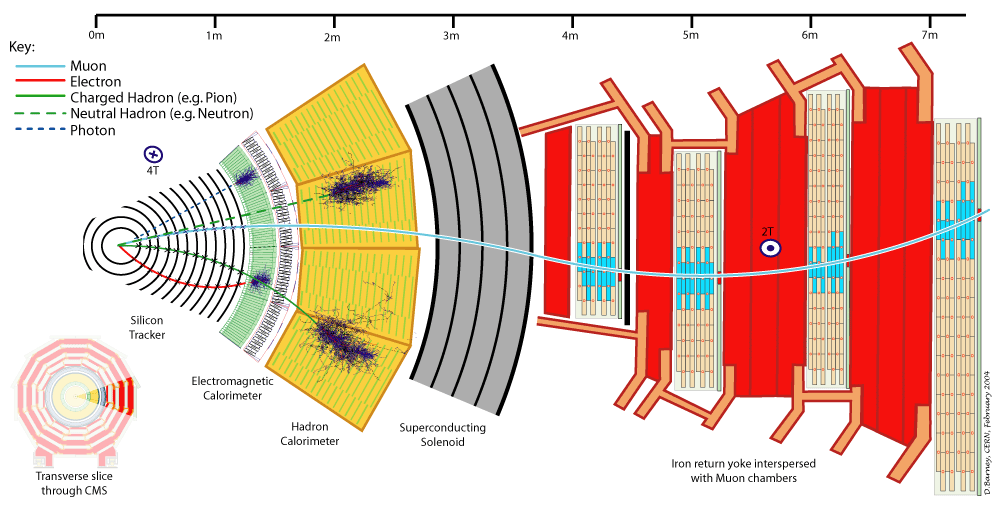
\includegraphics[scale=0.2]{THESISPLOTS/CMS_Slice.png}
%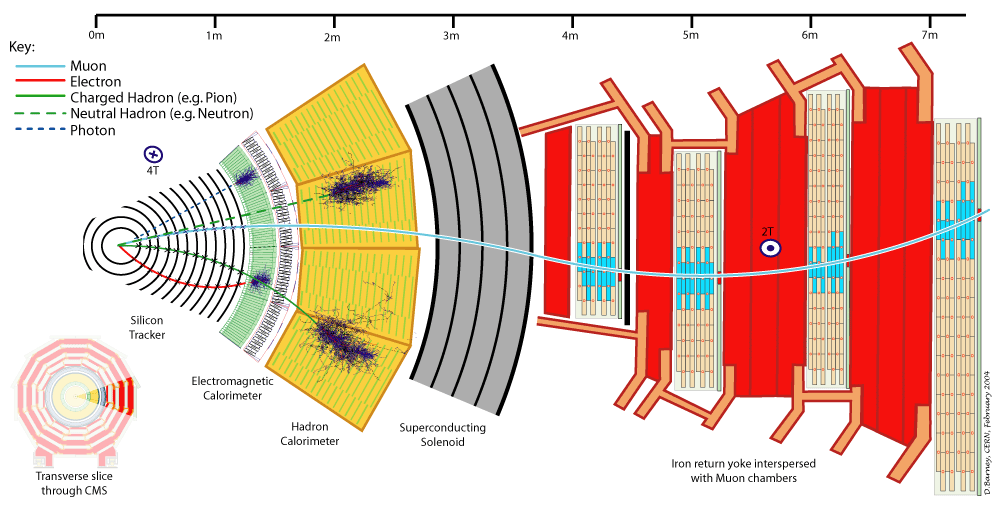
\includegraphics[scale=0.2]{THESISPLOTS/CMS_Slice.png}
%\captionof{figure}{Figure showing \MET distributions for events with out-of-time and in-time photons. ${\MET}_{1}$ and ${\MET}_{2}$ definitions are given in context. }
%\label{fig:METS}
%\end{center}
\section{Event Selection}
Pair produced neutralinos from the decay of gluino or squarks allows for at least a photon, jets and large  \ETslash\hspace{0.15cm} to make up ours signal events with neutralino decay, $\tilde{\chi}^{0}_{1} \rightarrow \gamma + \tilde{G}$. As a result, we select events with the required photon arrival time, number of jets(jet multiplicity) and \ETslash\hspace{0.15cm}. A cut in \ETslash\hspace{0.15cm} is particular useful in eliminating $\gamma + $ jets and QCD events with \ETslash\hspace{0.15cm} arising from finite missing transverse energy resolution or poor instrumentation also known as \textit{fake} \ETslash\hspace{0.15cm}. Event selection in jet multiplicity helps reduces background events not produced from the nominal proton-proton collisions like cosmic muons and machine induced events like beam halo muons and spikes. These events usually produce out-of-time photons.
\newline
Another possible background events are events with the decay of $\PW \rightarrow e + \nu$ and $t\bar{t}$, where the top~($t$) decays to a $b$ quark and a \PW 100\% of the time. We call these background events ElectroWeak~(EWK) events. These events also have fake photons(misidentified electrons as a photon) with real \ETslash\hspace{0.15cm} arising from the presence of the neutrinos~($\nu$). A cut in the photon \pt since we require high \pt photons and our multijet requirement of these events easily reduces this background.
\newline 
To reduce an equally good source of fake photons arising from multijets QCD events, where a jet is misidentified as photons, is reduced by requiring that the jets have very high \pt and are isolated Since jets from multijet QCD events are not always isolated.
\newline 
To reduce events from spikes and equally other fake photon events passing our required event selections, we only accept photons with ECAL time between $3 < t_{\gamma} < 13$~ns as our signal acceptance region.  And to reduce background contributions from ghost/satellite bunch collisions, we only select photons in the barrel~($|\eta_{\gamma}| < 1.479$) region of ECAL.
%%%
%%%
\subsection{Trigger Selection}
Our pre-event selection begins at the online where we select only events passing our online higher level trigger~(HLT). The HLT trigger used for our $\sqrt{S} = 8$~TeV proton-proton collision analysis is the \texttt{HLT\_DisplacedPhoton65\_CaloIdVL\_IsoL\_PFMET25} 
seeded by \texttt{HLT\_L1SingleEG12} level 1 trigger. This trigger was developed primarily for the study of delayed photons. To avoid bias in event selection towards any particular model, this trigger only requires that an accepted event contains an isolated photon with a \pt threshold of 65\GeVc and \ETslash\hspace{0.15cm} above 25\GeV. The minor axis of the photon electromagnetic shower must not be spread across many crystals in $\phi$, $ 0.1 < S_{\mbox{Minor}} < 0.4$. The trigger efficiency and turn-on curve~(efficiency becomes close to 100\%) for selecting  events with delayed photon candidates is done in photon \pt and \ETslash\hspace{0.15cm} selection variables. In order to avoid any correlation between the photon and \ETslash\hspace{0.15cm} variables, the efficiency for each variable is studied separately using another trigger \texttt{HLT\_Photon50\_CaloIdVL\_IsoL}.  The photon candidates used in this photon efficiency study must pass our offline photon selection criteria shown in table \ref{tab:PhotonSel}. The HLT photon selection efficiency for \pt is defined as the fraction of offline reconstructed photons to those triggered by \textit{HLT\_IsoPhoton50} photon candidates within $\Delta R < 0.5$.
% We do this by using a \texttt{SingleMuon} dataset~(\texttt{HLT\_IsoMu30}) to study the efficiency measurements.
Similarly, the \ETslash\hspace{0.15cm} HLT efficiency is defined as the fraction of events containing at least a jet and \ETslash\hspace{0.15cm} more than the HLT required \ETslash\hspace{0.15cm} of 25~GeV.
The results of the trigger efficiency measurements are shown in figure \ref{fig:HLTEff} against photon \pt and \ETslash\hspace{0.15cm}. These efficiency studies are made using the \texttt{HLT\_Photon50\_CaloIdVL\_IsoL} trigger which has no \ETslash\hspace{0.15cm}and jet multiplicity requirement  as the denominator and the \texttt{HLT\_DisplacedPhoton65\_CaloIdVL\_IsoL\_PFMET25} as numerator. A \texttt{SinglePhoton} dataset is used to verify these efficiency while and GMSB and $\gamma +$ jets samples is used to derive any correction factors between data and MC events.

\vspace{5mm}
\begin{minipage}{0.90\linewidth} 
\begin{center}
\mbox{
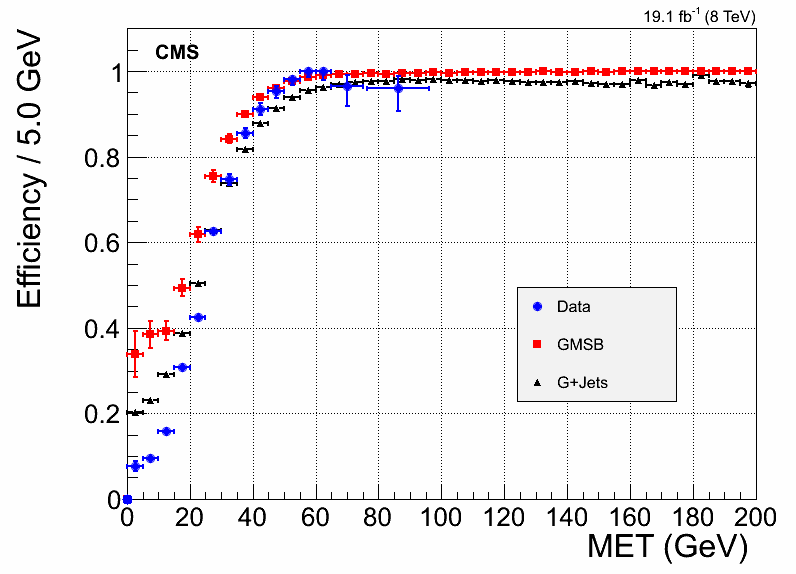
\includegraphics[height=0.45\textwidth, width=0.5\textwidth]{THESISPLOTS/PFMET_EffAsym.png}
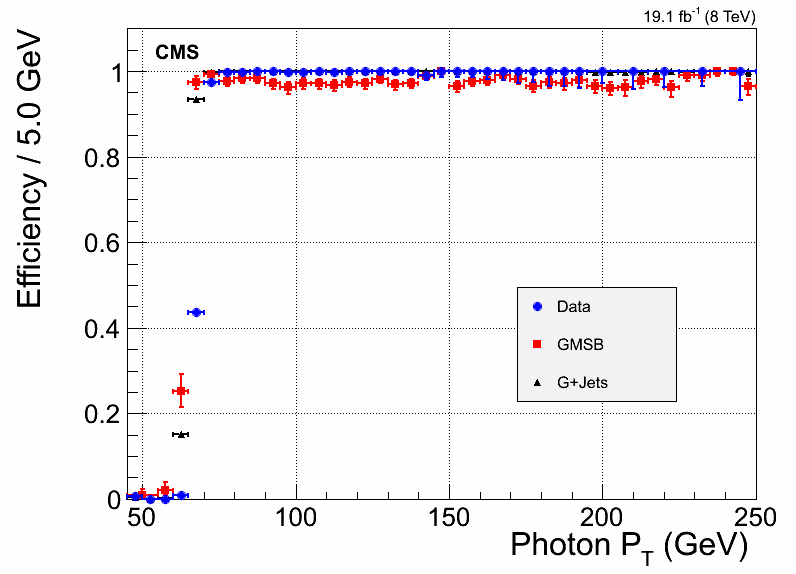
\includegraphics[height=0.45\textwidth, width=0.5\textwidth]{THESISPLOTS/Photon_EffAsym.png}}
\captionof{figure}{Trigger efficiency turn-on curves for photon \pt and $\MET > 25$\GeV~(left) and for \ETslash\hspace{0.15cm} with photon~(right).The $\gamma +$ jets samples require photon $\pt > 170$~\GeVc for selecting events with true \ETslash\hspace{0.15cm}.}
\label{fig:HLTEff}
\end{center}
\end{minipage}
%%%%
\subsection{Offline Selection}
In addition to the HLT selection, we apply an offline event selection on the photon, jets and \ETslash\hspace{0.15cm} of these events.
\newline
The leading photon of an event must have a \pt  greater than 80\GeVc while other photons candidates of the same event must have $\pt > 45\GeVc$. Because the particle flow~(PF) algorithm does not consider out-of-time isolated photon energy deposits, we do not use the PF photon isolation criteria but rather a \textit{simple cut-based} isolation requirement where we request that there should be no tracks near the selected photon within a range in $\Delta R(\gamma, track) < 0.6$, tracker, ECAL and HCAL isolation based on the photon \pt and \et must be within the accepted range required by the simple cut-based approach. The ration of the photon energy  deposited in HCAL to ECAL must be less than 5\% and the photon shower shape along the minor axis~($S_{\mbox{Minor}}$) must be be within 0.12 and 0.38. To prevent double counting with jets with high electromagnetic energy component, the photon must be isolated from any other particle in a cone size of  $\Delta R(\gamma, track)< 0.4$. 
We only selected photons belonging to the barrel~(EB) region \ie $|\eta_{\gamma}| < 1.479$ since we observed that an overwhelming large number of large ECAL time photon candidates from ghost/satellite bunch collisions belong to the endcap~(EE) as seen in Figure \ref{fig:TIMEECAL} of a photon ECAL time comparison between photon candidates belonging to EB and EE.
Our photon selection requirement is summarized in Table \ref{tab:PhotonSel}.
\newline
For jets, we select jets reconstructed with the PF algorithm based on the standard jet id selection criteria presented in Table \ref{tab:JetSel}. We require the leading jet in the event to have a \pt of at least 35\GeVc.
As for missing transverse energy~(MET) selection, with inspiration from our trigger event selection efficiency plot in MET in Figure \ref{fig:HLTEff}, we observed that a missing energy of at least 60\GeV for \ETslash\hspace{0.15cm} and ${\ETslash}^{\gamma}\hspace{0.15cm}$ is enough to suppress $\gamma + $ jets and QCD events with fake missing transverse energy.

\vspace{5mm}
\begin{minipage}{0.85\linewidth} 
\begin{center}
%\begin{table}[ht]
\centering
\begin{tabular}{l c }
\toprule
\multicolumn{2}{l}{\bfseries{Photon Selection Criteria}} \\
  \hline 
  \bfseries{Criteria} & \bfseries{Requirement} \\
   \hline 
   \toprule
 % \texttt{primary vertex number of tracks(vnof)}& $>= 4$ \\
 % \texttt{primary vertex transverse distance to beam}~($d0$) & $ < 2$~cm from CMS center \\
%  \texttt{primary vertex longitudinal distance to beam}~($|z|$) & $ < 24$~cm from CMS center \\
  \texttt{Event leading photon must have} $\pt(\gamma^{1})$  & $ > 80$~ GeV \\
  \texttt{Other photons in event must have} $\pt(\gamma^{>1})$  & $ > 45$~ GeV \\
 $|\eta_{\gamma}|$,(\texttt{Barrel Only}),  & $ < 3.0$ ($ < 1.5$) \\
 $S_{minor}$  & $ 0.12 \leq S_{Minor} \leq 0.38$ \\
 \textbf{H/E}  & $ < 0.05$ \\
 $\Delta R(\gamma, track)$  & $ > 0.6 $ \\
 HCAL Iso, ECAL Iso, Track Iso  & $ < 4.0 $, $ < 4.5 $, $ < 0.2 $ \\
 Photon Isolation cone size $\Delta R(\gamma, other particle)$ & $< 0.4$ \\
 Topological Spike cuts  & $1 - E_{6}/E_{2} < 0.98$, $ 1 - E_{4}/E_{1} < 0.98$ \\ 
  \hline 
  \bottomrule
\end{tabular}
\captionof{table}{The photon identification and selection  criteria used in this analysis}
\label{tab:PhotonSel}
%\end{table}
\end{center}
\end{minipage}

\vspace{5mm}
\begin{minipage}{0.85\linewidth} 
\begin{center}
%\begin{table}[ht]
\centering
\begin{tabular}{l c }
\toprule
\multicolumn{2}{l}{\bfseries{Jet PF identification selection criteria}} \\
  \hline 
  \bfseries{Criteria} & \bfseries{Requirement} \\
   \hline  
   \toprule
\texttt{Jet} \pt & $ > 35$\GeV \\
 \texttt{Number of Jet constituents} & $ > 1$ \\
 \texttt{Charge EM energy fraction~(CEF) } & $ > 0.99$ \\
 \texttt{Neutral Hadron energy fraction~(NHF) } & $ < 0.99$ \\
 \texttt{Neutral EM energy fraction~(NEF) } & $ < 0.99$ \\
 \texttt{If} $|\eta|$ \texttt{of jet is} $ >2.4$, \texttt{Charge Hadron energy fraction~(CHF) } & $ > 0$ \\
 \texttt{If} $|\eta|$ \texttt{of jet is} $ >2.4$, \texttt{Charge multiplicity~(NCH) } & $ > 0$ \\
 $\Delta R(\gamma, jet) = \sqrt{(\phi_{\gamma}-\phi_{jet})^{2} + (\eta_{\gamma}-\eta_{jet})^{2}}$ & $ > 0.3$ \\
 \toprule
 \texttt{\ETslash \hspace{0.25cm}, ${\ETslash}^{\gamma}\hspace{0.15cm}$} & $ > 60\GeV$ \\
\hline
\bottomrule
\end{tabular}
\captionof{table}{The Jet ID and MET selection used in this analysis}
\label{tab:JetSel}
%\end{table}
\end{center}
\end{minipage}

\vspace{5mm}
\begin{minipage}{\linewidth} 
\begin{center}
\centering
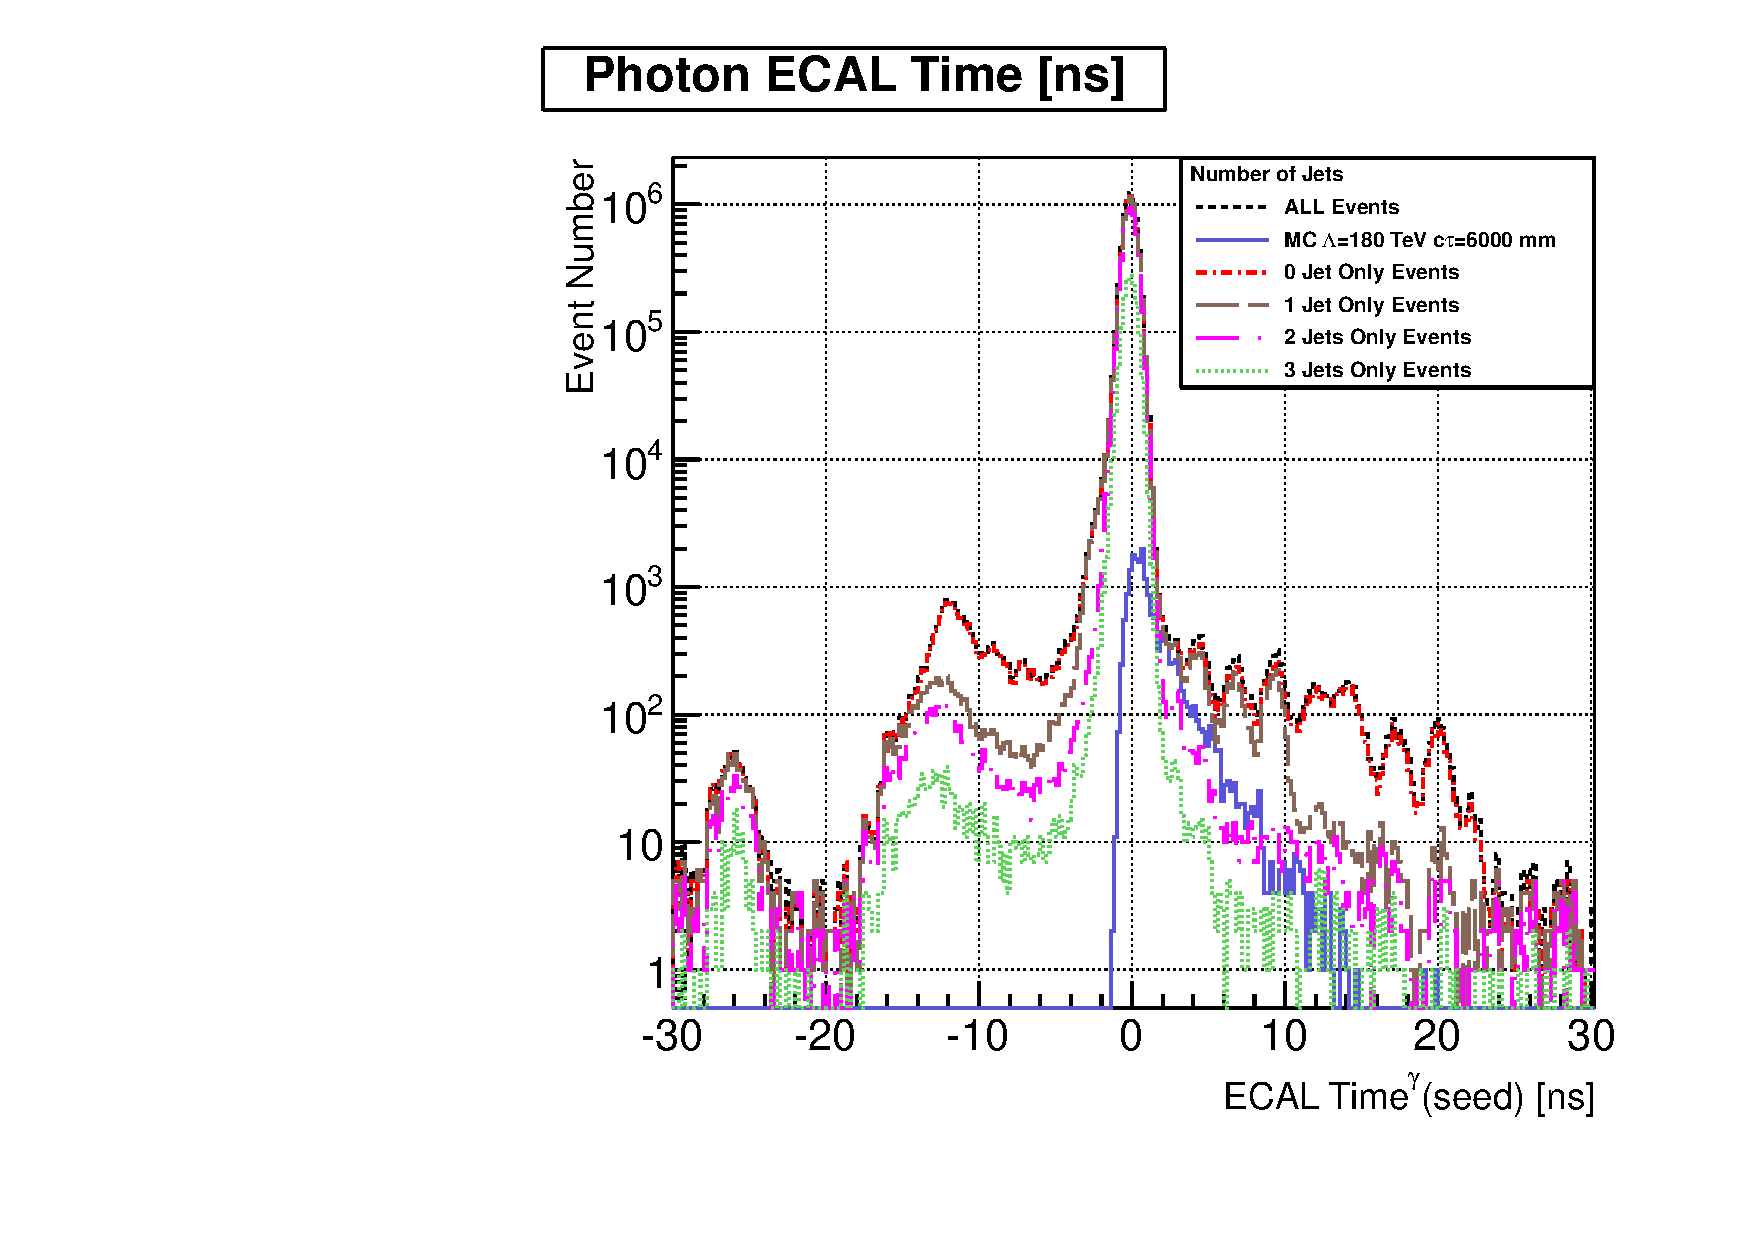
\includegraphics[height=0.65\textwidth, width=0.8\textwidth]{THESISPLOTS/Photon_SeedXtalTime_Distribution_VsJetMultiplicity.pdf}
\captionof{figure}{Photon with $\pt > 60$\GeV from data ECAL time distribution of events with different jet multiplicity and a single GMSB sample.}
\label{fig:TimePlotJet}
\end{center}
\end{minipage}

\vspace{5mm}
\par
  In summary, our signal events should have $\ge1~\gamma + \ge2~ jets + \ETslash\hspace{0.15cm} > 60\GeV + {\ETslash}^{\gamma}\hspace{0.15cm} > 60\GeV$. 
We use control samples(zero and one jet events since these events dominate our background sample, see Figure \ref{fig:TimePlotJet}) to test our background estimation method.

%%%$$$

\section{Background Estimation}
The main source of background is not from photon candidates produced in normal $pp$ collisions but rather from out-of-time photon candidates arising from non-collisions. To understand these out-of-time background events, we compare in-time~($|t_{\gamma}| < 1$~ns) photon candidates to out-of-time~($t_{\gamma} < -3$~ns and $t_{\gamma} > 2$~ns) photon candidates.
We also compare photons candidates from different jet multiplicity events to better understand the different background sources and their contributions. In Figure \ref{fig:BKGPLOTS}, we present scatter plots of the photon's ECAL time against $\eta$~(left) and against $\phi$~(right) for photons passing a loose~($\pt < 60\GeV$, barrel and endcap inclusive, $\ETslash\hspace{0.15cm} > 25\GeV$) event selection criteria.

\vspace{5mm}
\begin{minipage}{0.90\linewidth} 
\begin{center}
\centering
\mbox{
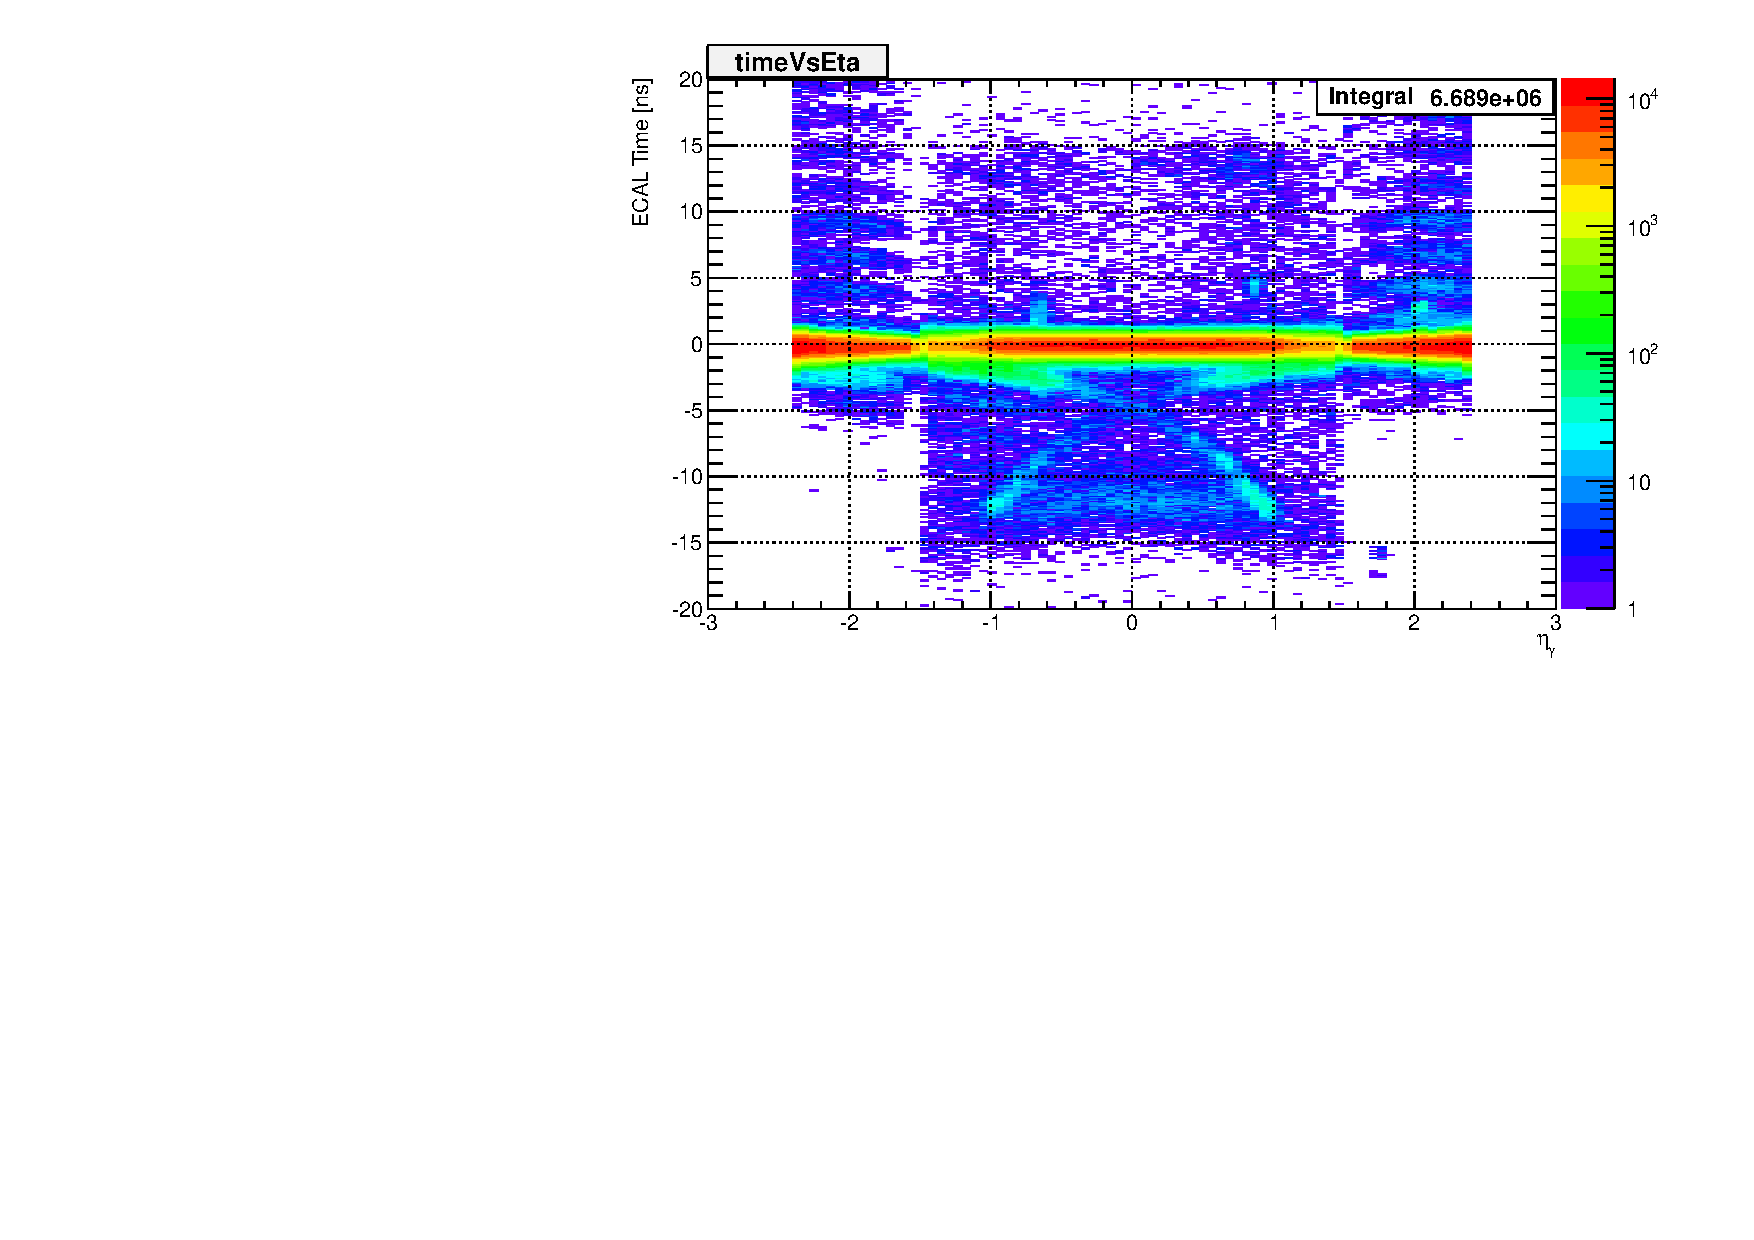
\includegraphics[height=0.4\textwidth, width=0.5\textwidth]{THESISPLOTS/SinglePhotonDataSet-TimeVsEta.pdf}
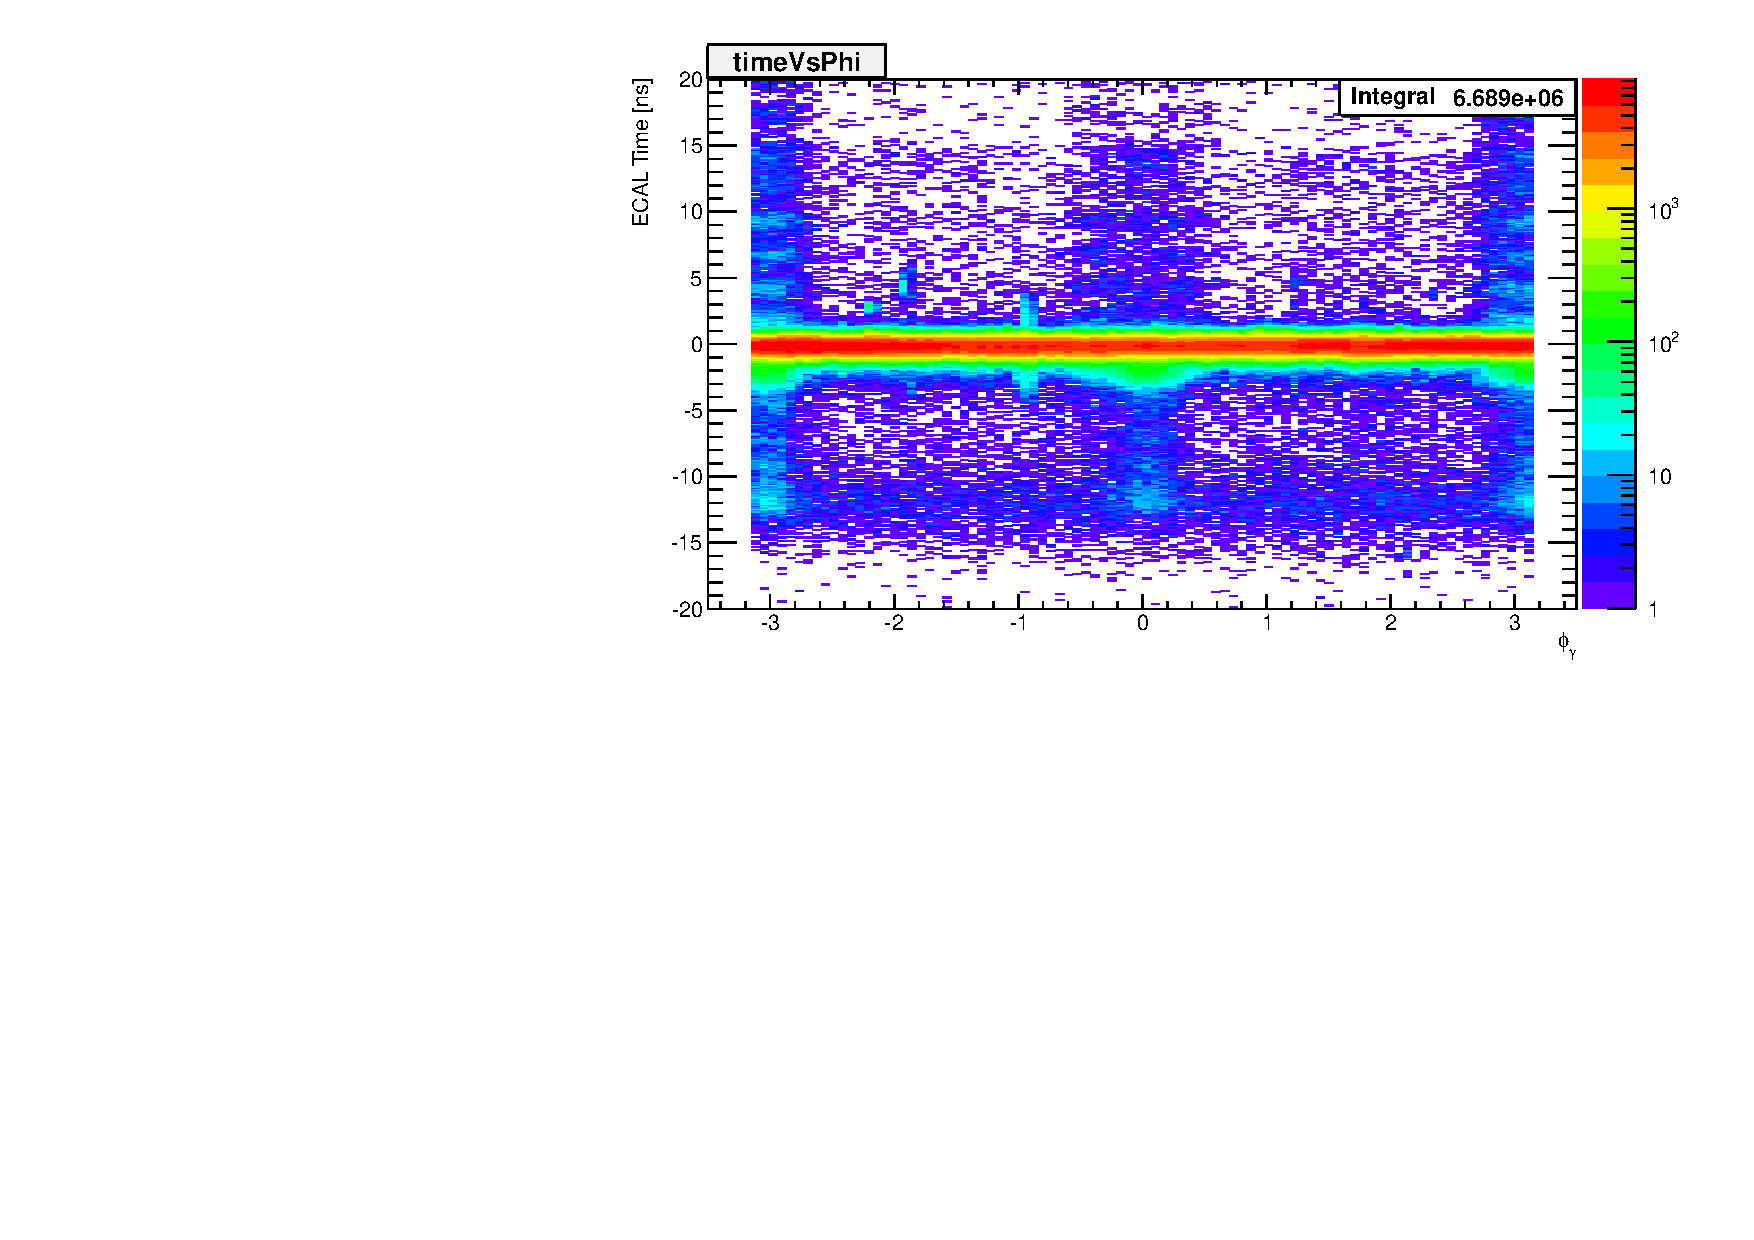
\includegraphics[height=0.4\textwidth, width=0.5\textwidth]{THESISPLOTS/SinglePhotonDataSet-TimeVsPhi.pdf}}
\captionof{figure}{ECAL time against $\eta$~(left) and ECAL time against $\phi$~(right) for photons with $\pt > 60$\GeV from data.}
\label{fig:BKGPLOTS}
\end{center}
\end{minipage}

\vspace{5mm}
 We observe that, although most of the photons arrive with ECAL time about zero, a good number of photon candidates possibly from very different sources, for example the cross-like feature seen in the plot on the left, have large ECAL time. We conclude that the possible sources of background photon candidates with large ECAL time measurements are mainly from beam halo muons, cosmic muons and spikes. A small addition also comes from photon candidates arising from ghost/satellite bunch collisions and some QCD events. To avoid, an irreducible contribution from spikes overpopulating a region with photon time , $t_{\gamma} \approx -12$~ns,  we restrict our definition for out-of-time photons to photons with ECAL time $ 2.0 < t_{\gamma} < 13.0$~ns and $ -10.0 < t_{\gamma} < -3$~ns. As a result, we only search for signal events with photon(s) having ECAL time between $2.0 < t_{\gamma} < 13.0$~ns, with at least $2$ jets and large \ETslash\hspace{0.15cm}.
\newline
 In our background estimation study, we first identify and reject photon candidates from beam halo, cosmic muons and spikes and then estimate the residual non-collision and collision background photon candidates  using the \textbf{\textsf{ABCD}} background estimation technique. 

\subsection{Collision Background}
\subsubsection{QCD Photons}
Events from satellite/ghost proton bunches spaced in $5.0$~ns or $2.5$~ns described in section \ref{Ghost}, produce out-of-time photons which can be present in EB. We refer to these photons as QCD photons. It is challenging to define a strategy for eliminating this background. Our approach, after rejecting non-collsiion events, was to estimate their contribution to signal using the \textsf{ABCD} background estimation method. Using \PZ events, we perform an additional background estimation of large ECAL time photon candidates from collision confirming our expectation that contribution from QCD photon events including true $pp$ collisions events is almost negligible. More on this is discussed in future sections.
%%%%
\subsection{Non-Collision Background}
Non-collision background events mainly cosmic muons, beam halo muons and spikes, have photons with large reconstructed time and large \ETslash\hspace{0.15cm} measurements. The high \pt photons from these energetic muons and possible overlapping  pile up events from multiple $pp$ collisions, contribute to the total sum of the PF reconstructed \pt imbalance leading to their large \ETslash\hspace{0.15cm} and at times jets associated with these events.
We select events with at least one good vertex, zero or one jet, photons satisfying ECAL spike cleaning, associated with candidate muons satisfying DT time cosmic muon cleaning and CSC tight halo-muon cleaning requirements to study these non-collision events. 
A schematic diagram in Figure \ref{fig:NeutDecay} show the production of photons from both non-collision and collision{ghost/satellite} in a typical LHC $pp$ collision within the CMS detector. Also shown is a typical photon from a neutralino decay in the GMSB model. Still on the diagram is shown the point of entry of beam halo muons into the CMS detector comparing to what is observed in the photon ECAl time against $\eta$ and $\phi$ plots of Figure \ref{fig:BKGPLOTS}.

\vspace{5mm}
\begin{minipage}{0.90\linewidth} 
\begin{center}
\captionsetup{type=figure}
\mbox{
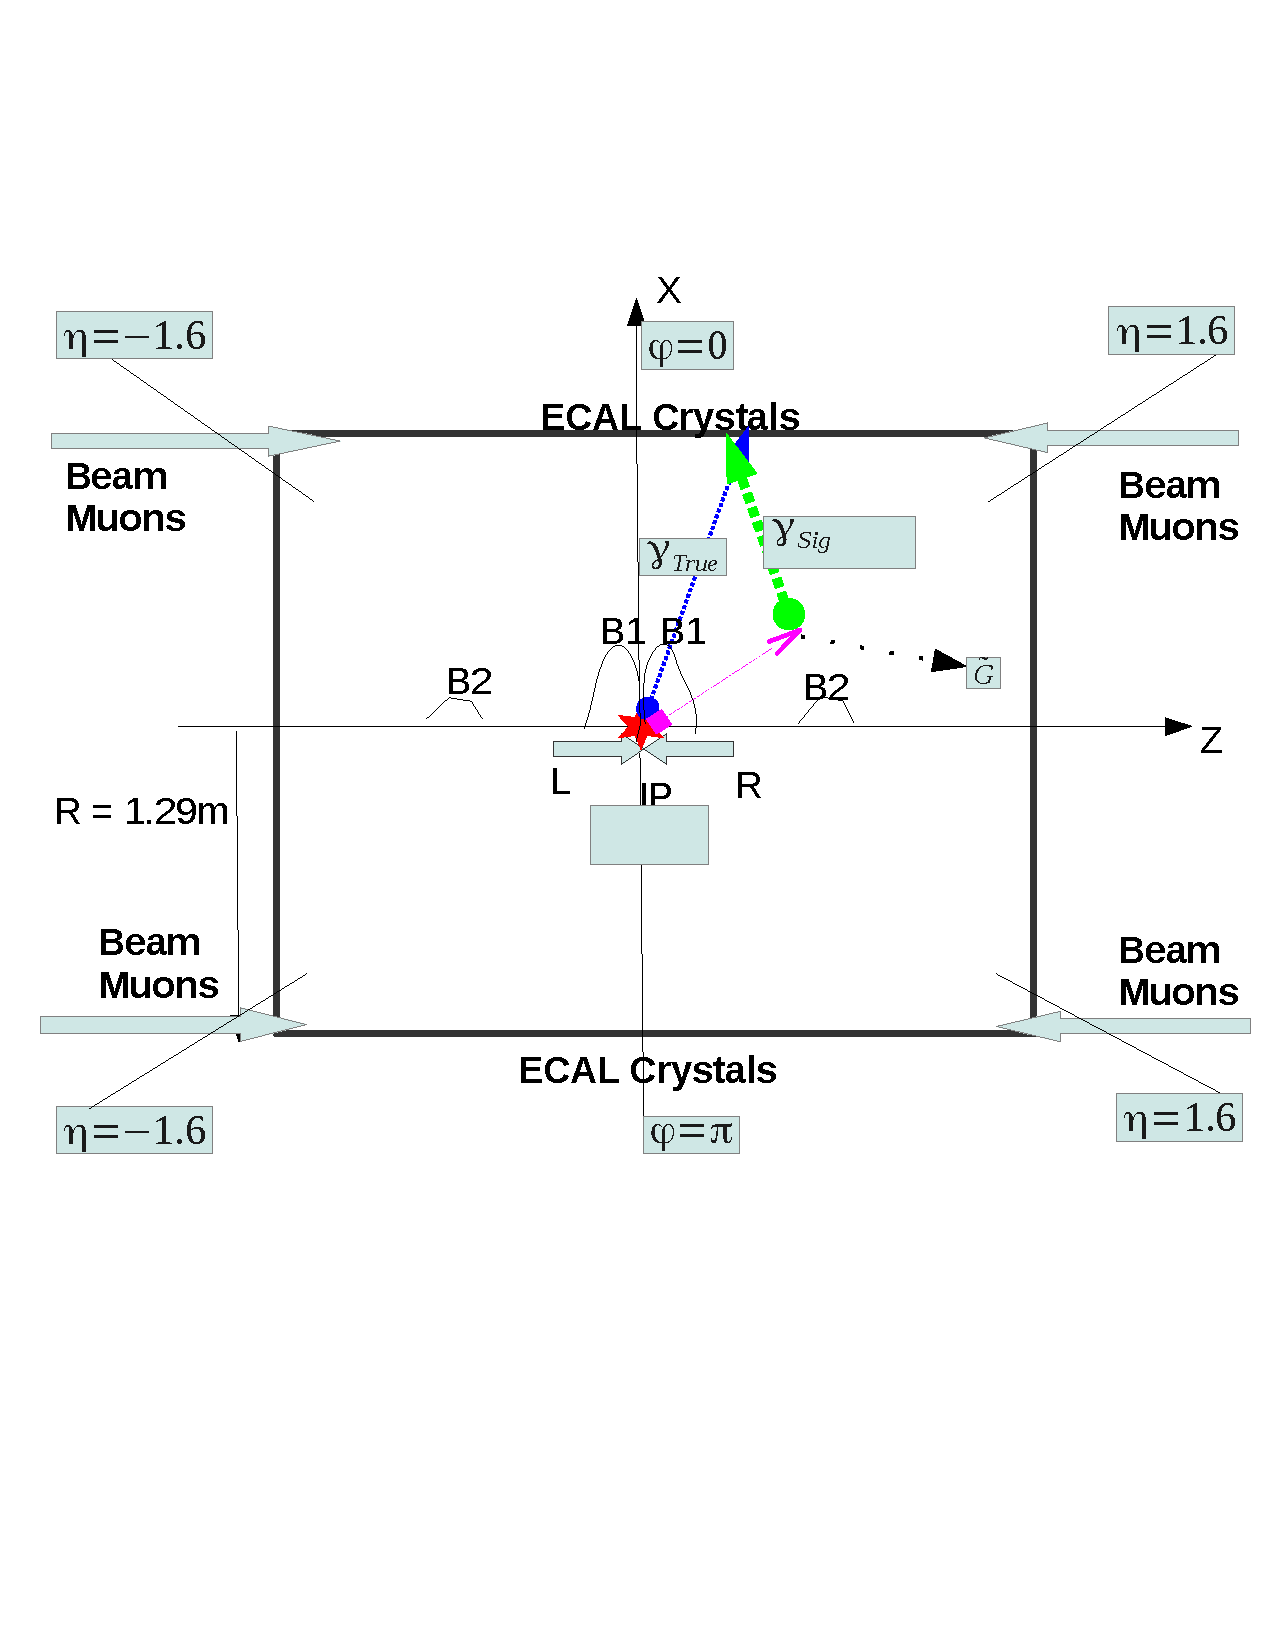
\includegraphics[height=0.35\textwidth, width=0.5\textwidth]{THESISPLOTS/Background_Delayed_Photon.pdf}
}
\captionof{figure}{Schematic diagram showing production of photons from main $pp$ and possible ghost/satellite bunch collisions in the CMS detector volume. Typical beam halo muon's entry direction into ECAL and GMSB neutralino decay is shown.}
\label{fig:NeutDecay}
\end{center}
\end{minipage} 
%%%%%

\subsubsection{Halo Photons}
  Protons in the main and ghost/satellite bunches can scatter off tertiary collimators~(TCT) about $z = 150$\m from CMS interaction point producing pions which later decay into muons traveling with energy of about a few \TeV. These energetic muons bremsstrahlung in the calorimeter detectors producing high energy photons called \textit{Halo photons}. Halo photons can also arise from energetic muons produced through inelastic scattering  of the protons in the colliding bunches with residual gas molecules of gases like H2, $CO_{2}$ in beam pipe about 550\m up from interaction  point~(IP).
These halo producing protons although traveling parallel with the main proton bunch stir away from the nominal orbit in the transverse direction due to betatron oscillations. Despite beam cleaning, there still remains a good amount of them present  and capable of producing energetic photons in ECAL spreading mostly in the horizontal plane as can be seen in the photon ECA time $v.s$ $\phi$ scatter plot presented in the right plot of Figure \ref{fig:BKGPLOTS}. In general, events arising from  beam related activities are referred to as \textit{Machine Induced Background}~(MIB) or \textit{Beam-Induced Background}~(BIB) events. The rate of halo photons in BIB events depends on the beam current and the operational conditions of the LHC, like the  machine optics, collimator settings, residual gas densities and filling scheme. 
\newline
The halo muons in BIB events, although having slightly lower energy than the main proton beams, equally travel parallel to the proton beam but are deflected most by the deflecting magnets. This deflection is mostly in the horizontal plane and the muons before entry into the ECAL, produce hits which can be reconstructed into muon tracks using segments in the Cathode Strip Chambers~(CSC) Endcap muon detectors. The reconstructed hits in CSC segments can be associated with the halo photon supercluster in ECAL within some narrow region in $\phi$. The geometry of ECAL allows most of the halo muons in the ECAL endcap regions with a few in the barrel. The resulting halo photons are usually out-of-time compared to photons produced directly from nominal $pp$ collisions. Most of the halo photons have earlier arrival time and their arrival time can be estimated from the unique flight path of the halo muons. We estimated the halo muon arrival time in ECAL with respect the arrival time of photons from $pp$ collisions as 
\begin{equation}{\label{eq:HALOPATH}}
t^{\mbox{expected}}_{\mbox{ECAL}} = -1/c\left( \pm Z_{\mbox{cluster}} + \sqrt{Z^{2}_{\mbox{cluster}} + R^{2}_{\mbox{cluster}}}  \right)
\end{equation}
where $Z_{\mbox{cluster}}$ is the point where the halo muon hits ECAL or longitudinal distance along $z$-axis from nominal interaction point, $R$ is the radial distance of the cluster from the beam line which is $1.29$\m and $c$ is the speed of light. Our estimated halo muon ECAL arrival time shown in Figure \ref{fig:HALO}, as the two red lines, agree well with the observed halo photon arrival ECAL time especially for earlier arrival time photons. It is much better to see this agreement once the expected halo muon arrival time equation is re-arrange to show its explicit dependence on $\eta$, which is the point of entry in ECAL given as
\begin{equation}{\label{eq:HALOPATH2}}
t^{\mbox{expected}}_{\mbox{ECAL}} = - \frac{R}{2c} \exp^{(-\eta)}
\end{equation} 
\par
By matching halo muon hit positions in CSC segments to photon supercluster positions in the ECAL calorimeter in $\phi$, since halo muons spread mostly in the horizontal or azimuthal~($\phi$) direction by the deflecting magnets, we are able to associated halo muons to their corresponding halo photons. We use the variable, $\Delta\phi(\mbox{CSC Seg},\gamma)$, which is the difference in $\phi$ between CSC segment  and the photon supercluster position in ECAL. A distribution of $\Delta\phi(\mbox{CSC Seg},\gamma)$ for in-time and out-of-time photons in the left plot of Figure \ref{fig:HALO} show that out-of-time photons have small $\Delta\phi(\mbox{CSC Seg},\gamma)$.

\vspace{5mm}
\begin{minipage}{0.90\linewidth}  
\begin{center}
%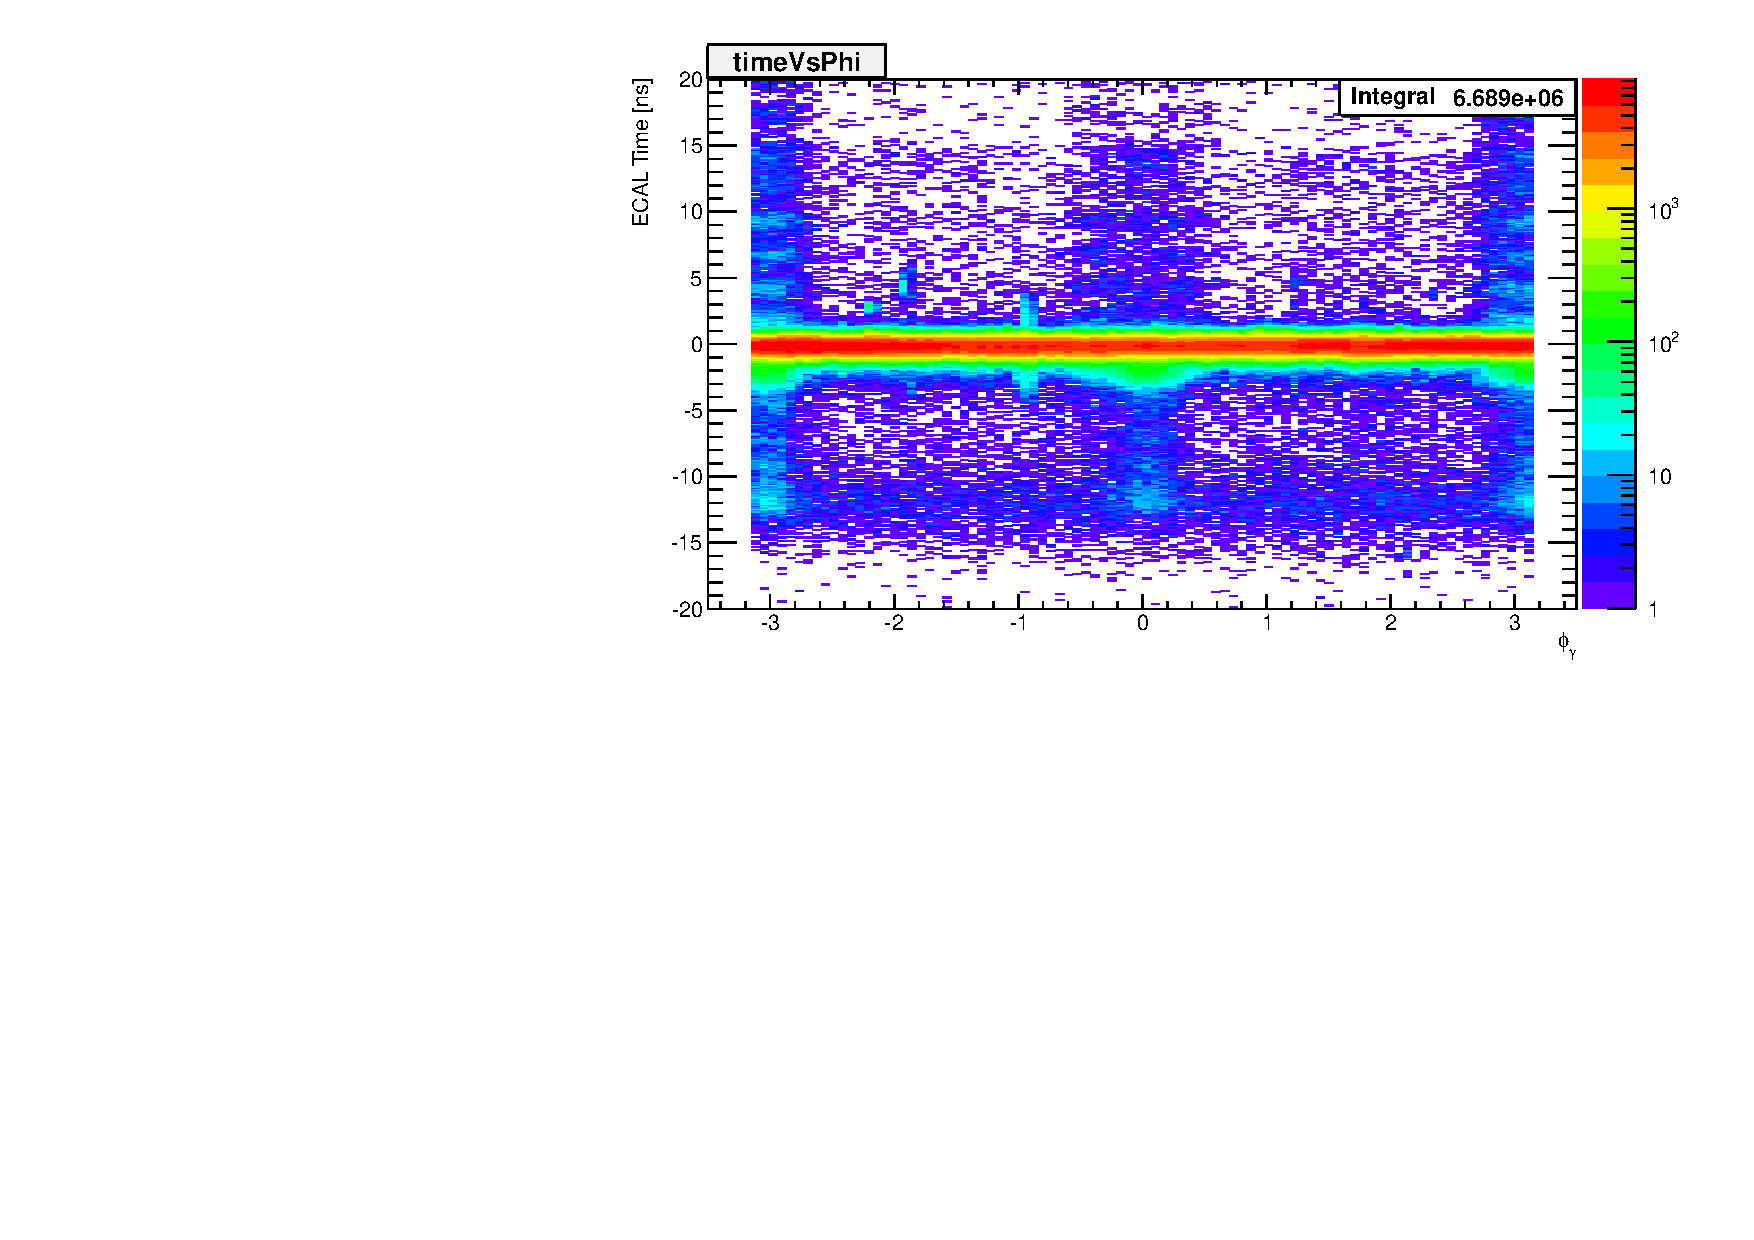
\includegraphics[height=0.35\textwidth, width=0.5\textwidth]{THESISPLOTS/SinglePhotonDataSet-TimeVsPhi.pdf}}
\mbox{
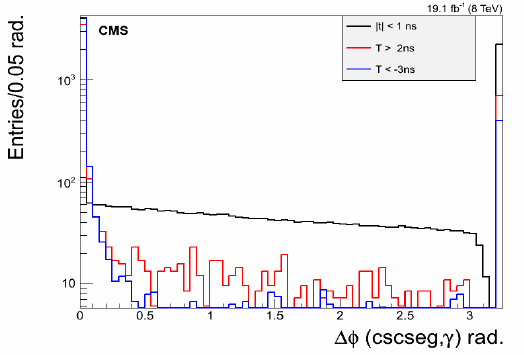
\includegraphics[height=0.45\textwidth, width=0.5\textwidth]{THESISPLOTS/CSC-Segment-Halo-Tagging.png}
%{THESISPLOTS/CSC_Segment_Halo_data.png}
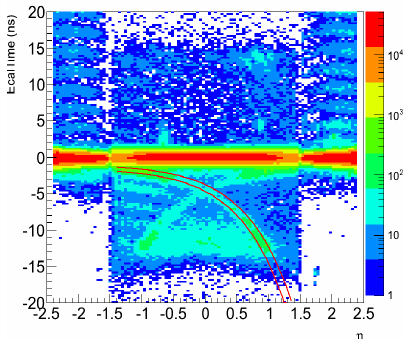
\includegraphics[height=0.45\textwidth, width=0.5\textwidth]{THESISPLOTS/HALO-ECAL-TIME-Vs-ETA.png}}
\captionof{figure}{(Left) ECAL time $V.s$ $\Delta\phi(\mbox{CSC Seg},\gamma)$ for in time(black) and out-of-time(red and blue) photons. (Right)Photon ECAL time $V.s$ $\eta$, expected halo photon time is shown as two red lines.}
\label{fig:HALO}
\end{center}
\end{minipage}

\vspace{5mm}
To estimate the performance of using $\Delta\phi(\mbox{CSC Seg},\gamma)$ for halo tagging, we use a halo photon candidate sample by selecting photons with $\phi_{\gamma}$ around $\phi = 0, \pm \pi$ and in the endcaps where we expect mostly halo photon candidates.  We were able to tag a good number of photon candidates as halo photons in the endcaps shown in the Figure \ref{fig:HALOENDCAP} comparing halo photons in EE with tagged halo photons in EE  with $\Delta\phi(\mbox{CSC Seg},\gamma) < 0.05$.
 
\begin{minipage}{0.90\linewidth} 
\begin{center}
\centering
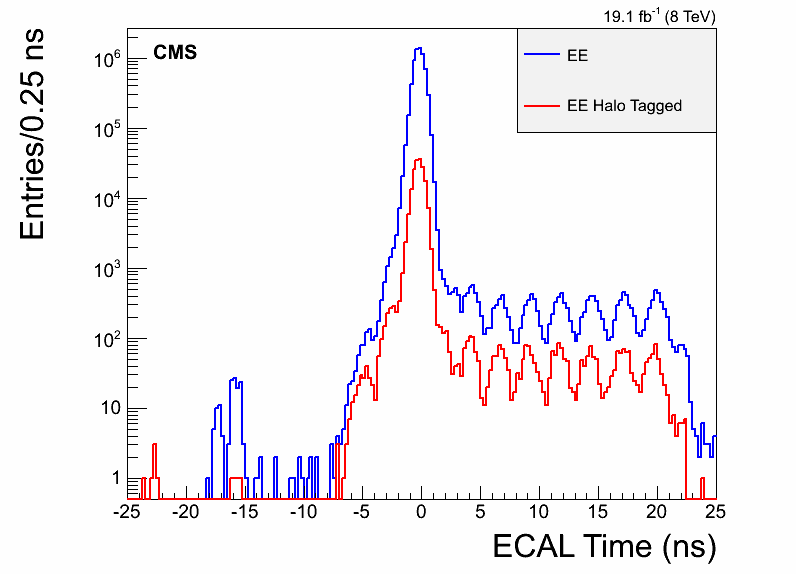
\includegraphics[height=0.45\textwidth, width=0.7\textwidth]{THESISPLOTS/halo_EE_Time.png}
\captionof{figure}{Using $\Delta\phi(\mbox{CSC Seg},\gamma) < 0.05$ to tag photons with $\phi_{\gamma} = 0, \pm \pi$ in the endcaps. A good portion of endcap photon candidates are tagged.}
\label{fig:HALOENDCAP}
\end{center} 
\end{minipage}

\subsubsection{Cosmic Photons}
Cosmic muons like beam Halo muons with sufficient energy  will also radiate~(bremsstrahlung) photons in in ECAL. We refer to these photons as \textit{cosmic photons}. Unlike halo muons, cosmic muons can arrive at ECAL from any direction. Cosmic photons in the barrel are expected to be produced from cosmic muons with hits in the Drift Tubes~(DT) segments. Using DT segments and  photon supercluster $\eta-\phi$ position in ECAL, we can match cosmic muon hits in DT segments to ECAL photon superclusters within $\Delta\eta$ and $\Delta\phi$. The DT position used in calculation of $\Delta\eta$ and $\Delta\phi$ is a projection of the muon trajectory using the direction of the DT segment to the outer surface of ECAL due to the large space between the muon barrel and the ECAL. The two dimensional distribution for $\Delta\eta(\mbox{DT Seg},\gamma)$ and $\Delta\phi(\mbox{DT Seg},\gamma)$ of this matching for events with out-ot-time photons; $t_{\gamma} > 2$~ns and $t_{\gamma} < -3$~ns is shown in the right plot of Figure \ref{fig:COSMIC}. We compared to $\Delta\eta(\mbox{DT Seg},\gamma)$ and $\Delta\phi(\mbox{DT Seg},\gamma)$ distribution for in-time~($|t_{\gamma}| < 1$~ns), shown in the left plot, still in Figure \ref{fig:COSMIC}, we observed that most out-of-time photons have a small $\Delta\eta$ and $\Delta\phi$. Comparing the $\Delta\eta$  and $\Delta\phi$ 2-dimensional distributions of these out-of-time photons to photons from a pure cosmic muons sample~(data taken when no proton-proton collisions is happening), we found a similar small $\Delta\eta$ and $\Delta\phi$ occupancy by true cosmic muons sample, shown in Figure \ref{fig:TRUECOSMIC}. We conclude that small $\Delta\eta(\mbox{DT Seg},\gamma)$  and $\Delta\phi(\mbox{DT Seg},\gamma)$ can be used to tag and reject events with cosmic photons.

%\paragraph*{}\mbox{}\\
\begin{minipage}{0.90\linewidth} 
\begin{center}
\mbox{
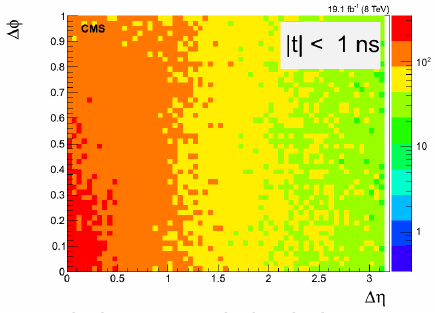
\includegraphics[height=0.45\textwidth, width=0.5\textwidth]{THESISPLOTS/Cosmic_In-time-Photons_Data.png}
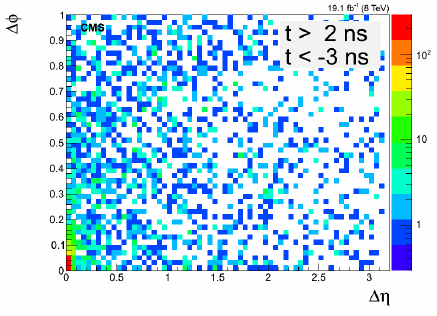
\includegraphics[height=0.45\textwidth, width=0.5\textwidth]{THESISPLOTS/Cosmic_Out-Of-time-Photons_Data.png} 
}
\captionof{figure}{Scatter plot showing $\Delta\eta(\mbox{DT Seg},\gamma)$ against $\Delta\phi(\mbox{DT Seg},\gamma)$ for out-of-time~($ t_{\gamma} > 2$~ns and $t_{\gamma} < -3$~ns) photons(Right) compared to in-time($|t_{\gamma}| < 1$~ns) photons(Left). Cosmic photon candidates occupy the small $\Delta\eta$ and $\Delta\phi$ region.}
\label{fig:COSMIC}
\end{center}
\end{minipage}

%\paragraph*{}\mbox{}\\
\begin{minipage}{0.90\linewidth} 
\begin{center}
\mbox{
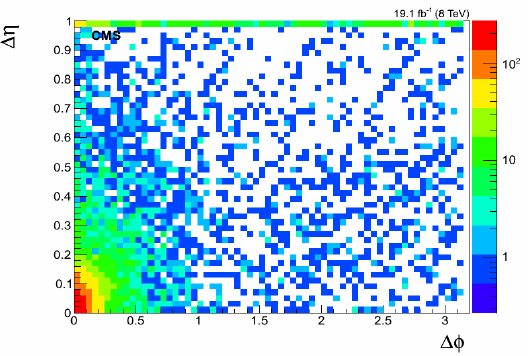
\includegraphics[height=0.45\textwidth, width=0.6\textwidth]{THESISPLOTS/Cosmic_Ray_Photons_Cosmic_dataset.png} }
\captionof{figure}{Scatter plot of $\Delta\eta(\mbox{DT Seg},\gamma)$ against $\Delta\phi(\mbox{DT Seg},\gamma)$ for photons from pure cosmic muon data. Small $\Delta\eta$ and $\Delta\phi$ are cosmic photons.}
\label{fig:TRUECOSMIC}
\end{center}
\end{minipage}

\subsubsection{Anomalous Photons: Spikes}
Neutrons and charge hadrons can at times deposit their energy directly to the APDs rather than through crystal scintillation. The signals read from the APDs are \textit{anomalous}  and referred to as \textit{spikes}. Spikes are produced from $pp$ collisions and can be easily misidentified for real isolated photons passing photon selection criteria. A spike supercluster consists of very few crystals; most often one or two crystals. Spikes can also overlapped with real photons and found embedded in a real photon supercluster or buried inside high electromagnetic fraction jets. Such embedded spikes are difficult to identify. By looking at the signal pulse height, the pulse shape for a spike signal appear different from a real photon signal. As a result, reconstructed ECAL time for spikes usually have a large calculated $\chi^{2}$ value.
\newline
Because of the absence of crystal scintillation, the arrival time of spikes is much earlier~(negative), usually about $t \approx -12.0$~ns than true photons produced in nominal $pp$ collisions with crystal scintillation. The few crystals containing the spike cluster energy deposits makes is possible for spikes to be easily identified using a energy topological selection variable, $1-\frac{E_{4}}{E_{1}}$, also know as \textit{swiss-cross} variable.  By looking at a distribution of  the swiss-cross for in-time and a spike candidate sample(mostly photons with time $t = -12$~ns, shown in right plot of Figure 
\ref{fig:SPIKES}, we observed than most spikes have about 98\% os their energy deposited in a single crystal.
Using the number of crystals in photon supercluster and comparing in-time photons to a beam halo photons and spike candidate photons~(see left plot in Figure \ref{fig:SPIKES}), we confirmed that most spikes including spikes embedded in electromagnetic candidates have less than $7$ crystals in their supercluster. A combination of the swiss-cross, number of crystals in supercluster, calculated $\chi^{2}$, $S_{\mbox{major}}$ and $ S_{\mbox{minor}}$~(both $S_{\mbox{major}}$ and $ S_{\mbox{minor}}$ describe the shape of the electromagnetic shower), are useful in identifying and rejecting events with spikes.

\vspace{5mm}
\begin{minipage}{0.90\linewidth} 
\begin{center}
\captionsetup{type=figure}
\mbox{
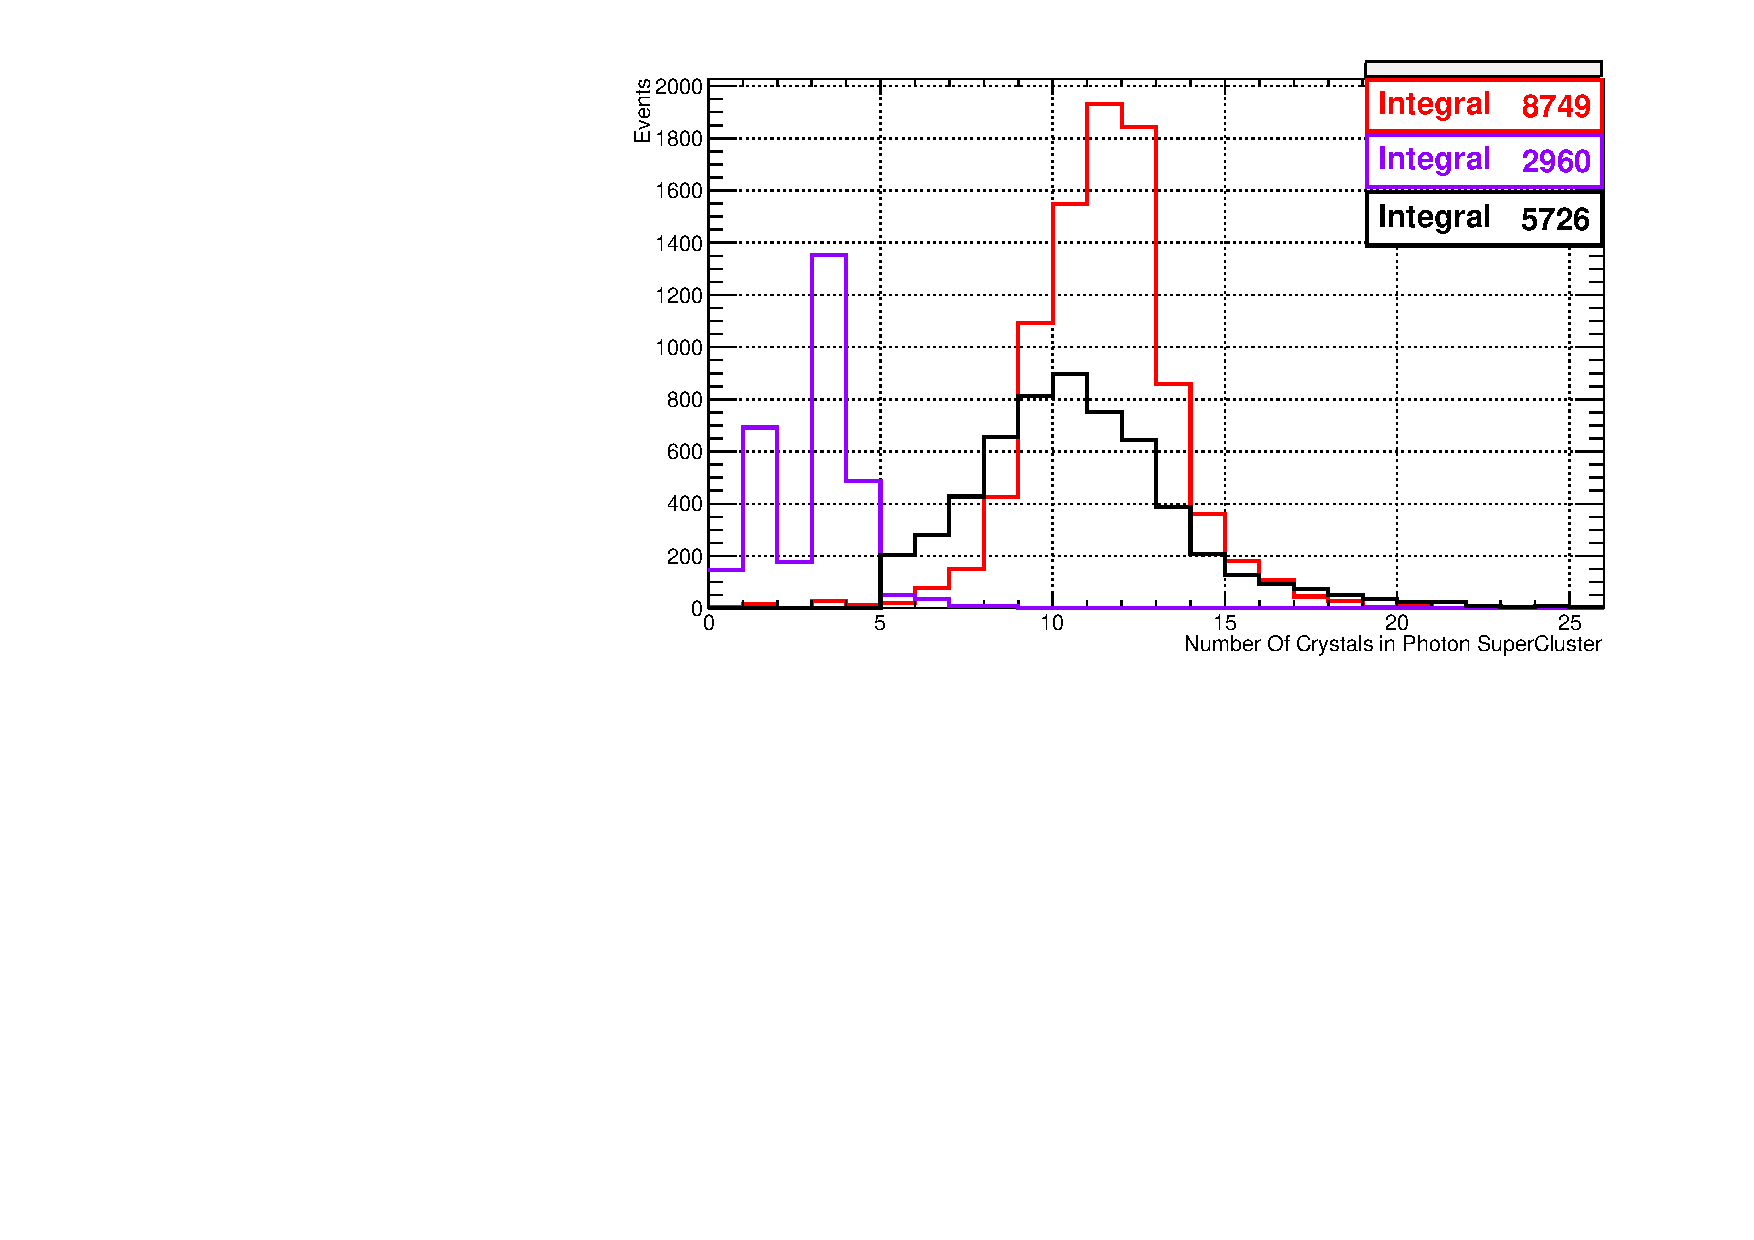
\includegraphics[height=0.50\textwidth, width=0.5\textwidth]{THESISPLOTS/Number-Of-Crystals-In-Photon-SC.pdf}
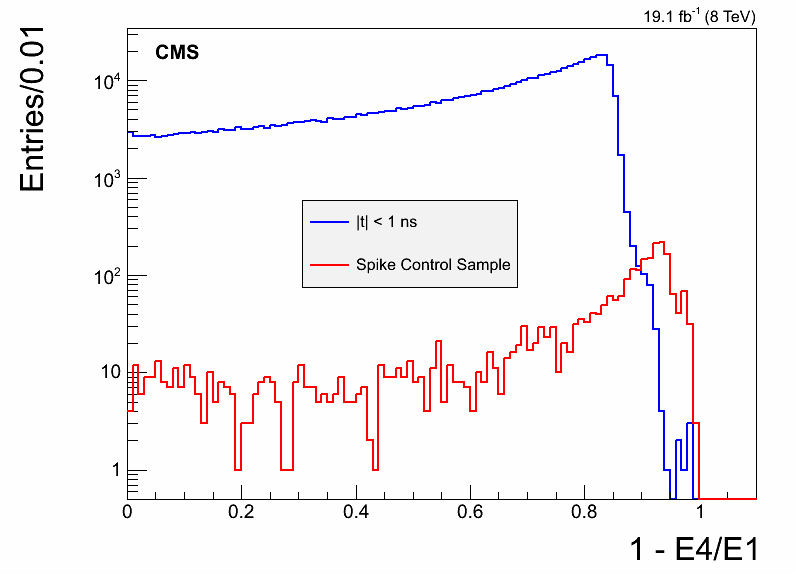
\includegraphics[height=0.50\textwidth, width=0.5\textwidth]{THESISPLOTS/swissX.png} }
\captionof{figure}{\textit{Number of crystals} in photon supercluster plot~(Left) for real photons candidates(black), spike photon candidates~(magenta) and halo photon candidates~(red). The spike photon candidates are selected with an energy swiss-cross variable~($1- E_{4}/E_{1}$)~(Right) shown comparing in-time photons~($|t_{\gamma}| < 1.0 $) to spike candidate sample.}
\label{fig:SPIKES}
\end{center}
\end{minipage}

\subsection{Event Cleaning, Veto Performance and Fake Rates}
Using the selection variables studied above for halo, cosmic and spike photons, we tag and reject non-collision events as follows: 
\begin{itemize}
\item Beam halo photons are tagged and rejected if a CSC segment with $|\eta| > 1.6$ is found within 0.05 radian of the azimuthal angle with a photon supercluster, \ie photons found within $\Delta\phi(\mbox{CSC Seg},\gamma) < 0.05$ are rejected. We found that we are able to reject halo photons with 91\% efficiency and 3\% mis-tag rate using this photon selection requirement.
\item Cosmic photons are tagged and rejected with $75.5$\% efficiency and $1.4$\% mis-tag rate for photons associated with DT segments within $\Delta\eta(\mbox{DT Seg},\gamma) < 0.1$ and $\Delta\phi(\mbox{DT Seg},\gamma) < 0.1$.
\item Most of spikes are rejected if the photons has $\chi^{2} > 4$, $\mbox{Number of Crystals} < 7$ and $ 1-E_{4}/E_{1} > 0.98$, with only $0.4$\% mis-tag rate.
\end{itemize}
Our full veto performance in terms of mis-tag rate for the different non-collision background sources studied  is summarized in Table \ref{tab:EVTC}.

%%\paragraph*{}\mbox{}\\
\begin{minipage}{0.90\linewidth} 
\begin{center}
\begin{tabular}{|c| c|}
%\mbox{Fake Rate }
\hline
\bfseries{Background Source} & \bfseries {Fake Rate}(\%)\\
\hline\hline
\textit{Halo Photons} & ~$\approx 3$ \\
\textit{Cosmic Muons} & ~$\approx 1.4$ \\
\textit{Spikes} & $\approx 0.4$ \\
\hline
\end{tabular}
\captionof{table}{Fake rates for different non-collision cleaning.}
\label{tab:EVTC} 
\end{center}
\end{minipage}

\vspace{5mm}
The result of our tagging of the different types of non-collision background events can be seen in Figure \ref{fig:RESIDUAL}. Halo photons produced from the so-called beam halo muons are the majority of our background out-of-time photon events. Very few late arrival time photons are produced from spikes while there is also some significant contribution from cosmic photons. The most interesting is the residual out-of-time background(in red) which could not be tagged. 

\paragraph*{}\mbox{}\\
\begin{minipage}{0.90\linewidth} 
\begin{center}
  \captionsetup{type=figure}
   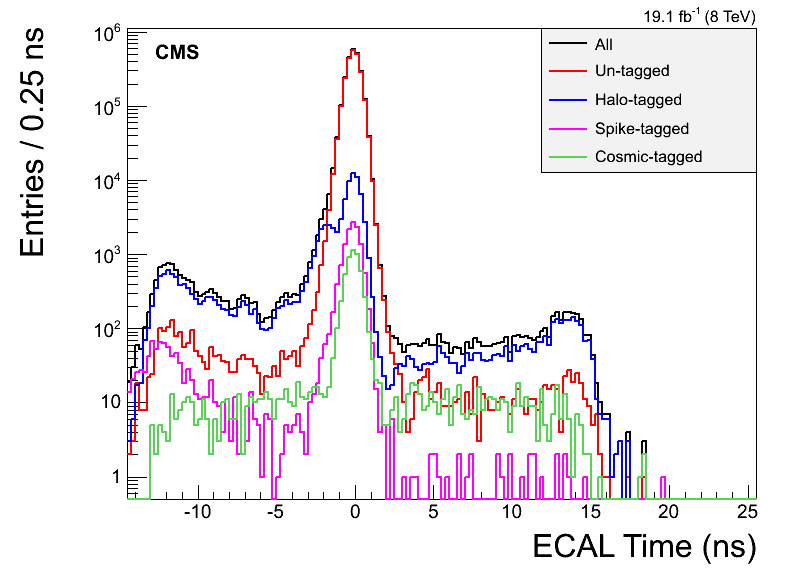
\includegraphics[height=0.7\textwidth, width=0.8\textwidth]{TimeForAll}
%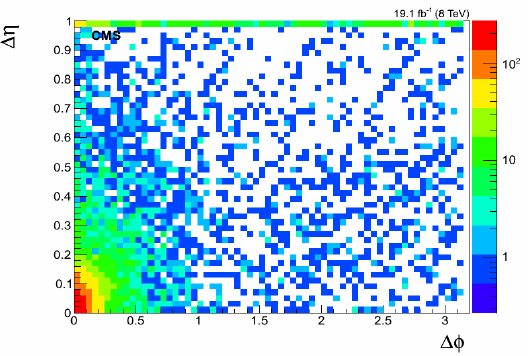
\includegraphics[height=6cm, width=0.5\textwidth]{THESISPLOTS/Cosmic_Ray_Photons_Cosmic_dataset.png} 
   \captionof{figure}{ECAL Photon time for a data sample of 0 and 1-jet events showing our tagging performance for non-collision background events.}
   \label{fig:RESIDUAL}
\end{center}
\end{minipage}

\vspace{5mm}
It is possible that the contributions to the residual out-of-time photon events are from 
mistagged non-collision events since the tagging efficiency is not 100\% efficient, ghost or QCD collision events with out-of-time photons, events with $\PW\rightarrow \Pe\Pagne$ decays with misidentified electron as photon passing the photon selection, or signal events with real delayed photons. To better understand these various contributions, we use the missing transverse energy,${\ETslash}^{\gamma}\hspace{0.15cm}$ and $\ETslash\hspace{0.15cm}$, recalling that $\vec{{\ETslash}^{\gamma}\hspace{0.15cm}} = \vec{\ETslash\hspace{0.15cm}} + \vec{\pt^{\gamma}}$ adjusting for out-of-time energy deposits not included in the standard missing transverse energy calculations. 
\newline
Signal events because of the undetected gravitino from the neutralino decay will have large ${\ETslash}^{\gamma}\hspace{0.15cm}$ and $\ETslash\hspace{0.15cm}$ and events with $\PW\rightarrow \Pe\Pagne$ decay will also have ${\ETslash}^{\gamma}\hspace{0.15cm}$ and $\ETslash\hspace{0.15cm}$ because of the undetected neutralino. Non-collision(cosmic, halo, spike) and collision~(ghost/sattelite or QCD) events can be separated into high-\pt and low-\pt events.
High-\pt Non-collision events will have large $\ETslash\hspace{0.15cm}$ attributed mostly due to the exclusion of energy deposits from the out-of-time photons in the missing transverse energy reconstruction and small ${\ETslash}^{\gamma}\hspace{0.15cm}$ when the large transverse energy contribution from energy deposits of the out-of-time photons is re-introduced. Low-\pt Non-collision events will have both ${\ETslash}^{\gamma}\hspace{0.15cm}$ and $\ETslash\hspace{0.15cm}$ small since the out-of-time photon transverse energy excluded was not large in the first place. For high-\pt out-of-time collision events, these events naturally have low missing transverse energy so automatically $\ETslash\hspace{0.15cm}$  is required to be small while after re-introducing the energy deposits from out-of-time high-\pt photons, then ${\ETslash}^{\gamma}\hspace{0.15cm}$ becomes large. With the same argument for low-\pt Non-collision events, low-\pt collision events are expected to have both small  ${\ETslash}^{\gamma}\hspace{0.15cm}$ and $\ETslash\hspace{0.15cm}$.
A table showing a summary of our expectations for ${\ETslash}^{\gamma}\hspace{0.15cm}$ and $\ETslash\hspace{0.15cm}$ of different background events source contributing to the residual out-of-time photon untagged events is presented in Table \ref{tab:METSAMPLE}.

\vspace{5mm}
\begin{minipage}{0.90\linewidth} 
  \begin{center}
   \begin{tabular}{c| c|c}
   \toprule
     \bfseries{Event Sample} & \bfseries{$\ETslash\hspace{0.15cm}$} &          \bfseries{${\ETslash}^{\gamma}\hspace{0.15cm}$}\\
    \toprule
     \hline
     Signal Events & Large & Large \\
     $\PW\rightarrow \Pe\Pagne$ Events & Large & Large \\
     High-\pt Non-Collision(Mostly Beam Halo) Events & Large & Small \\
     Low-\pt Non-Collision Events & Small & Small \\
     High-\pt Collision(QCD/Ghost) Events & Small & Large \\
     Low-\pt Collision Events & Small & Small \\
     \hline
   \bottomrule     
   \end{tabular}
   \captionof{table}{Summary of missing transverse expectation for events with out-of-time photons.}
   %\caption{\textsf{ABCD} Control Regions~(CRs) for estimating non-collision background.}
   \label{tab:METSAMPLE} 
 \end{center}
\end{minipage}

\vspace{5mm}
Therefore, to minimizing contributions from events anomalous photon time, we restrict our photon arrival time for signal events to within $3.0 < t_{\gamma} < 13.0$~ns, while also requiring that the signal event missing transverse energy be greater than 60\GeV, \ie ${\ETslash}^{\gamma}\hspace{0.15cm} > 60$\GeV, $\ETslash\hspace{0.15cm} > 60$\GeV. This reduces the contribution from ghost/satellite background contributing to the untagged out-of-time photons while at the same time enhances our signal event sample.
Using events from $pp$ collisions with predominantly in-time~($ -2.0 < t_{\gamma} < 2.0$~ns) photons, 
events with $t_{\gamma} > 3.0$~ns and $t_{\gamma} < -3.0$~ns, we define control samples in different \ETslash\hspace{0.15cm} and also small ${\ETslash}^{\gamma}\hspace{0.15cm}$ event selection regions enhancing either collision or non-collision background events and perform an \textsf{ABCD} background estimation method with the goal of estimating the total expected number of background events with out-of-time photons with $t_{\gamma} > 3.0$~ns.
\par
We verify out background estimation technique using a data sample of zero and one jet events where the expected and observed number of events with out-of-time photons, $t_{\gamma} > 3.0$~ns and  ${\ETslash}^{\gamma}\hspace{0.15cm} > 60$\GeV, $\ETslash\hspace{0.15cm} > 60$\GeV  is supposed to be the same if the method is valid. One of our assumption for using the ABCD method is that the background contributions from QCD events and multijets events is negligible. We also study the consequences of this assumption on the number of background estimated events with a separate control sample of mostly out-of-time photon candidates used in reconstructing the true \PZ mass and measure the its candidate electron's arrival time at ECAL since for these events we expect most of the electrons from the $\PZ \rightarrow \EE$ decay to be in-time. Thus, the observed number of out-of-time electron candidates gives us an estimate of the contributions of collision events in our signal sample.
 
%%\begin{figure}[htbp]
%%  \begin{center}
%%    \captionsetup{type=figure}
%%     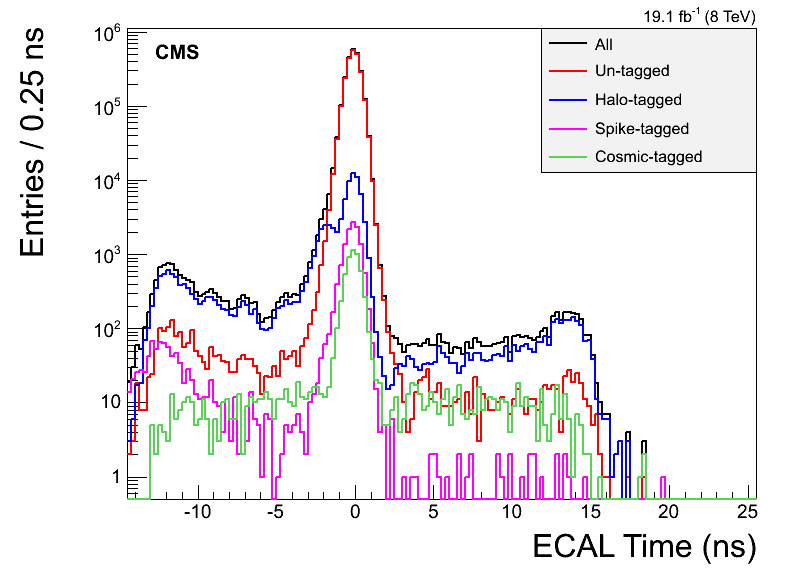
\includegraphics[height=0.7\textwidth, width=0.8\textwidth]{TimeForAll}
%%    \caption{Residual Background(red) after tagging the different non-collision background sources using the selection variables described in text.}
%%    \label{fig:RESIDUAL}
%%   \end{center}
%%\end{figure}
%%\begin{table}[h!]
%% \begin{center}
%%   \begin{tabular}{| l c r |}
%%   \hline
%%   1 & 2 & 3 \\
%%   4 & 5 & 6 \\
%%   7 & 8 & 9 \\
%%   \hline
%%   \end{tabular}
%% \end{center}
%%\caption{A simple table}
%%\end{table}
%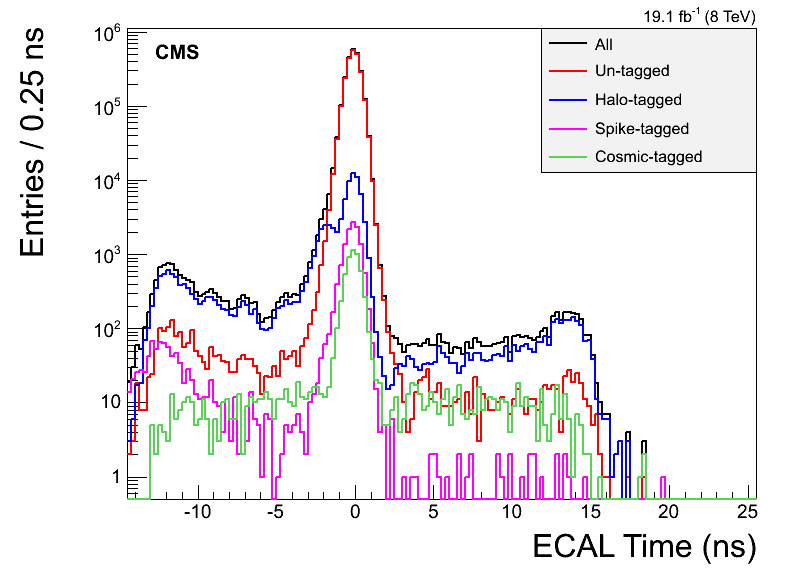
\includegraphics[height=0.7\textwidth, width=0.8\textwidth]{TimeForAll}
%\end{figure}
\subsection{Background Estimation with ABDC Method}
Since we expect most of our background events to come from non-collision events, we first estimate the number of events we expect from non-collision events using the \textsf{ABCD} technique and then estimate the possible contribution from collision events in the control samples used in our \textsf{ABCD} method.
\begin{enumerate}
\item \textbf{Non-Collision Background Estimation}:\newline
To estimate the number of background events from non-collision, we define \textsf{ABCD} Control Samples~(CS) in ECAL time and  ${\ETslash}^{\gamma}\hspace{0.15cm}$ by selecting events with $\ETslash\hspace{0.15cm} > 60$\GeV. Events with $\ETslash\hspace{0.15cm} > 60$\GeV is a CS for which the contribution from collision~(QCD) background is suppressed since most collision background events as seen in table \ref{tab:METSAMPLE} have small \ETslash\hspace{0.15cm}. The control samples \textsf{A} and \textsf{B} defined in Table \ref{tab:NON-COLLISION} as events

\vspace{5mm}
\begin{minipage}{0.90\linewidth} 
  \begin{center}
   \begin{tabular}{|c| c| c|}
   \hline
     \bfseries{Non-Collision} & $\mathbf{{\ETslash}^{\gamma}\hspace{0.15cm}} < 60$\GeV & $\mathbf{{\ETslash}^{\gamma}\hspace{0.15cm}} > 60$\GeV \\     
      \hline \hline
        $3.0 < t_{\gamma} < 13.0$~ns. &  \textsf{$C$} &  \textsf{$D$} \\
      \hline
        $ -10.0 < t_{\gamma} < -3.0$~ns & \textsf{$A$} &  \textsf{$B$} \\
    \hline 
   \end{tabular}
   \captionof{table}{\textsf{ABCD} Control Samples~(CSs) definitions for estimating non-collision background. Events must satisfy the $\ETslash\hspace{0.15cm} > 60$\GeV selection requirement.}
   %\caption{\textsf{ABCD} Control Regions~(CRs) for estimating non-collision background.}
   \label{tab:NON-COLLISION} 
  \end{center}
 \end{minipage}
%%\end{table}
%\begin{itemize}
%\item \textbf{A}: Events with ${\ETslash}$~~$ < 60$~GeV and $ -10.0 < t_{\gamma} < -3.0$~ns.
%\item \textbf{C}: Events with ${\ETslash}$~~$ < 60$~GeV and $3.0 < t_{\gamma} < 13.0$~ns.
%\item \textbf{B}: events with ${\ETslash}$~~$ > 60$~GeV and $-10.0 < t_{\gamma} < -3.0$~ns.
%\item \textbf{D}: events with ${\ETslash}$~~$ > 60$~GeV and $3.0 < t_{\gamma} <  13.0$~ns.
%\end{itemize}
\vspace{5mm}
 with photon time, $-10.0 < t_{\gamma} < -3.0$~ns, and \textsf{C} as events with ${\ETslash}^{\gamma}\hspace{0.15cm} < 60$\GeV 
and photon time  $3.0 < t_{\gamma} < 13.0$~ns, all do not contain signal events. Using these CS for the \textsf{ABCD}  method,  with the assumption that $\frac{N_{D}}{N_{C}} = \frac{N_{B}}{N_{A}}$, the number of non-collision background events with out-of-time photons expected in the signal  CS \textsf{D} is given as
\begin{equation}
N^{non-col}_{D} = \left(\frac{N_{B}}{N_{A}} \right)\cdot N_{C},
\end{equation}
where $N^{non-col}_{D}$ is the number of non-collision background events we expect in the \textsf{D} CS, $N_{B}$, $N_{A}$  and $N_{C}$ are the number of events observed in respectively \textsf{B}, \textsf{A} and \textsf{C} CSs.

\item\textbf{Collision Background Estimation}:\newline
In order to quantify how suppressed is the contribution from possible collision background events in each of the CSs defined in Table \ref{tab:NON-COLLISION}, we once again employ the \textsf{ABCD} technique by defining Control Samples~(CSs) in ECAL time and \ETslash\hspace{0.15cm}. Since we are interested in contributions into CS \textsf{B} and \textsf{D} of Table \ref{tab:NON-COLLISION}, as these are the only CS where we expect a sizable contribution from collision events~(see Table \ref{tab:METSAMPLE}), we select events with ${\ETslash}^{\gamma}\hspace{0.15cm} > 60$\GeV.
Most collisions events have photons with in-time~($|t_{\gamma}| < 2$~ns), therefore, we use CSs defined with in-time photons to estimate the number of possible collision events with out-of-time photons contributing to CSs \textsf{B} and \textsf{D}. The CSs used for the new \textsf{$A^{\prime}$ $B^{\prime}$ $C^{\prime}$  $D^{\prime}$} method to perform these estimations are defined as shown in Table \ref{tab:COLLISION}. 

\vspace{5mm}
\begin{minipage}{0.90\linewidth} 
\begin{center}
\begin{tabular}{|c| c| c|}
 \hline
\bfseries{Collision}       & $\mathbf{\ETslash\hspace{0.15cm} } < 60$\GeV &  $\mathbf{\ETslash\hspace{0.15cm}} > 60$\GeV \\      
\hline \hline
$3.0 < t_{\gamma} < 13.0$~ns. &  \textsf{$C^{\prime}$} &  \textsf{$D^{\prime}$} \\
\hline
$ -2.0 < t_{\gamma} < 2.0$~ns & \textsf{$I^{\prime}$} &  \textsf{$I$} \\
\hline 
$ -10.0 < t_{\gamma} < -3.0$~ns & \textsf{$A^{\prime}$} &  \textsf{$B^{\prime}$} \\
\hline
\end{tabular}
\captionof{table}{\textsf{$A^{\prime}$ $B^{\prime}$ $C^{\prime}$ $D^{\prime}$} and \textsf{$I$ $I^{\prime}$} control samples for estimating collision background. Events here must satisfy ${\ETslash}^{\gamma}\hspace{0.15cm} > 60$\GeV selection requirements. }
\label{tab:COLLISION} 
\end{center}
\end{minipage}

\vspace{5mm}
The number of collisions events contributing to the CSs \textsf{B}, $N_{B}^{col}$, is estimated as 
\begin{equation}{\label{eq:COLB}}
\displaystyle{N_{B}^{col} = N_{B^{\prime}}  = \left( \frac{I}{I^{\prime}} \right)\cdot N_{A^{\prime}}}, 
\end{equation}
while the number of events contributing to the CS \textsf{D}, $N_{D}^{col}$, is estimated according to
\begin{equation}{\label{eq:COLD}}
\displaystyle{N_{D}^{col} = N_{D^{\prime}}  = \left( \frac{I}{I^{\prime}} \right)\cdot N_{C^{\prime}}},
\end{equation}
where the general assumption is that $\frac{N_{B^{\prime}}}{N_{A^{\prime}}}  = \frac{N_{I}}{N_{I^{\prime}}}$ and  $\frac{N_{D^{\prime}}}{N_{C^{\prime}}}  = \frac{N_{I}}{N_{I^{\prime}}}$.
%\begin{itemize}
%\item $\mathbf{A^{\prime}}$: Events with ${\ETslash}^{\gamma} < 60$~GeV and $-10.0 < t_{\gamma} < -3.0$~ns.
%\item $\mathbf{B^{\prime}}$: Events with ${\ETslash}^{\gamma} > 60$~GeV and $-10.0 < t_{\gamma} < -3.0$~ns.
%\item $\mathbf{I^{\prime}}$: Events with ${\ETslash}^{\gamma} < 60$~GeV and $|t_{\gamma}| < 2.0$~ns.
%\item $\mathbf{I}$: Events with ${\ETslash}^{\gamma} > 60$~GeV and $|t_{\gamma}| < 2.0$~ns.
%\end{itemize}
%we also define a in time CR as:
%\begin{itemize}
%\item $\mathbf{C^{\prime}}$: Events with ${\ETslash}^{\gamma} < 60$~GeV and $ 3.0 < t_{\gamma} <  13.0$~ns.
% \item $\mathbf{D^{\prime}}$: Events with ${\ETslash}^{\gamma} > 60$~GeV and $3.0 < t_{\gamma} <  13.0$~ns.
% \item $\mathbf{I^{\prime}}$: Events with ${\ETslash}^{\gamma} < 60$~GeV and $|t_{\gamma}| < 2.0$~ns.
%\item $\mathbf{I}$: Events with ${\ETslash}^{\gamma} > 60$~GeV and $|t_{\gamma}| < 2.0$~ns.
%\end{itemize}
\item \textbf{Combined Background Estimation}: \newline
Now that we have estimates for both collision and non-collision event contributions, we can estimate the total number of background events expected our signal CS \textsf{D} which defines events with $\ETslash\hspace{0.15cm} > 60$\GeV, ${\ETslash}^{\gamma}\hspace{0.15cm} > 60$\GeV and $3.0 < t_{\gamma} < 13.0$~ns, as
\begin{equation}{\label{eq:FBKG}}
N_{D}^{Total} = \left(\frac{N_{B} - N_{B}^{col} }{N_{A}} \right)\cdot N_{C} + N_{D}^{col} = N_{D}^{non-col} + N_{D}^{col}
\end{equation}
where $N_{D}^{Total} = N_{D}^{non-col} + N_{D}^{col}$ is the total background events estimated in our signal CS \textsf{D} coming from non-collision and collision background events. 
\end{enumerate}
%\begin{center}
%\centering
%\mbox{
%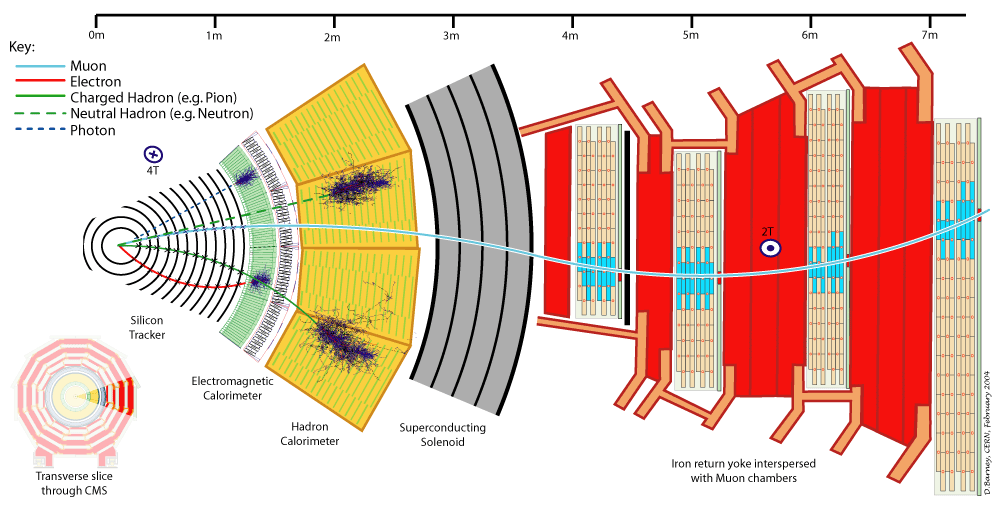
\includegraphics[scale=0.2]{THESISPLOTS/CMS_Slice.png}
%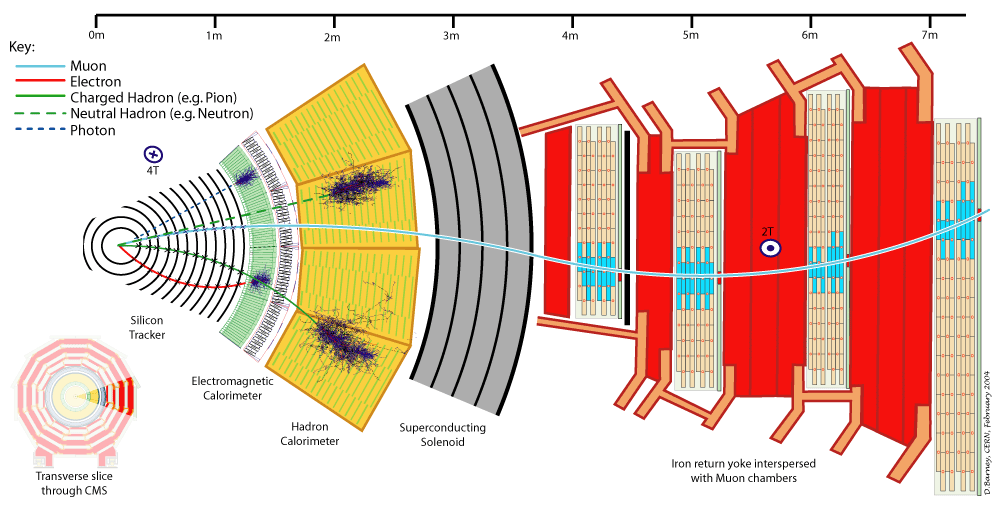
\includegraphics[scale=0.2]{THESISPLOTS/CMS_Slice.png}
%\captionof{figure}{Diagrams showing background estimation technique.}
%\label{fig:BKGESTI}
%\end{center}
\paragraph*{Background Estimation Technique Validation}\mbox{}\\
Using a data sample of $0$ and $1$-jet events where we do not expect any signal events, we performed closure test to validate the background estimation method described in the previous section.
The closure test checks for an agreement in the number of events expected obtained using our background estimation method and that observed in our signal CS \textsf{D}. The $0$ and $1$-jet events are required to satisfy the same event selection requirements as our signal event except for the number of jet criteria where only $0$ or $1$ events pass. The event yields in each control sample of the background estimation methods including the tagging of beam-halo, cosmic and spike events are shown in Table \ref{tab:EVTYIELD}.

\vspace{5mm}
\begin{minipage}{0.90\linewidth} 
\begin{center}
\begin{tabular}{c| c| c| c| c }
\toprule
 \hline
\bfseries{Control Sample} & Yield & Beam Halo & Cosmic & Spike \\
\hline
\toprule
\textsf{A} & 852 & 5075 & 237 & 65\\
\textsf{B} & 39 & 300&  17 &  1\\
\textsc{C} & 359 & 1508 & 368 & 9  \\
\textsf{D} & 10 & 22 & 30 & 0 \\
\hline\hline
\textsf{$A^{\prime}$}& 8 &  1& 1 & 0\\ 
\textsf{$C^{\prime}$}& 2 & 0 & 0 & 0\\  
\textsf{$I$} & 35464 & -& - & -\\    
\textsf{$I^{\prime}$}&  1446522 & - & - & \\       
\textsf{$B^{\prime}$}& - &-  & - & -\\    
\textsf{$D^{\prime}$}& - & - & - & -\\      
\hline
\bottomrule
\end{tabular}
\captionof{table}{Event yields used in closure test for the validation of \textsf{ABCD} background estimation method using $0$ and $1$-jet events sample. Beam halo/cosmic/spikes yields are obtained from tagged events.}
\label{tab:EVTYIELD} 
\end{center}
\end{minipage}

\vspace{5mm}
Using the yields in Table \ref{tab:EVTYIELD} for each CS and Equations \ref{eq:COLB}, \ref{eq:COLD} and \ref{eq:FBKG}, we obtain the following estimates for the expected number of events in signal CS \textsf{D} as
\begin{align*} 
 N_{B}^{col} &= \frac{35464}{1446522} \times 8 = 0.20^{+0.08}_{-0.06} \\
 N_{D}^{col} &= \frac{35464}{1446522} \times 2 = 0.05^{+0.05}_{-0.02} \\
 N_{D}^{Total} &= \left( \frac{39 - 0.20}{852}\times 359\right) +  0.05 = 16.40^{+3.04}_{-2.63}.
\end{align*}
The uncertainty are statistical uncertainties based on the event statistics in each CS. Our expected number of background events in signal CS \textsf{D} is $6.40^{+3.04}_{-2.63}$  which is, within the statistical uncertainties, agreeable with the 10 events we observed satisfying all our event selection requirements and belonging to the CS \textsf{D}. 
This give us confidence to now apply our background estimation method for our true data sample.
% We observed $10$ events while from using Equation \ref{eq:FBKG}, we expected $16.78^{+2.95}_{-3.45}$. We argue that within our statistical uncertainties, there is quite an agreement between our expectation and observed events. The complete result from our closure test is shown in Table \ref{tab:EVTC}. This gives us confidence that our  background estimation method is robust and reliable. We apply the same \textsf{ABCD} to estimate the background contribution in our signal sample. Our signal sample consist of events with at least $2$-jets, at least a single photon and ${\ETslash}^{\gamma}\hspace{0.15cm} > 60$\GeV, $\ETslash\hspace{0.15cm} > 60$\GeV
%\paragraph*{}\mbox{}\\
%\begin{minipage}{\linewidth} 
%\begin{center}
%\begin{tabular}{|c| c| c|}
%\mbox{Fake Rate }
%\hline
%\bfseries{Non-Collision} &  $\mathbf{{\ETslash}^{\gamma}\hspace{0.15cm}} < 60$\GeV & $\mathbf{{\ETslash}^{\gamma}\hspace{0.15cm}} > 60$\GeV \\
%\hline
% $3.0 < t_{\gamma} < 13.0$~ns & \textsf{C}($405$) & ~\textsf{D}($10$) \textcolor{blue}{16.78} \\
% $-10.0 < t_{\gamma} < -3.0$~ns & \textsf{A}($871$) & ~\textsf{B}($36$) \\
%\hline \hline
%\bfseries{Collision} & $\mathbf{\ETslash\hspace{0.15cm}} < 60$\GeV & $\mathbf{\ETslash\hspace{0.15cm}} %> 60$\GeV \\
%\hline 
% $3.0 < t_{\gamma} < 13.0$~ns & \textsf{$D^{\prime}$}($4$) & ~\textsf{D}($10$) \\
% $-2.0 < t_{\gamma} < 2.0$~ns & \textsf{$F^{\prime}$}($1353685$) & ~\textsf{F}($34543$) \\
% $-10.0 < t_{\gamma} < -3.0$~ns & \textsf{$B^{\prime}$}($5$) & ~\textsf{B}($36$) \\
%\hline 
%\end{tabular}
%\captionof{table}{Result from closure test of background estimation technique using 0 and 1-jet events. Numbers in bracket represent our expected background estimate using \textsf{ABCD} method.}
%\label{tab:EVTC} 
%\end{center}
%\end{minipage}
\subsection{Background Estimation Cross Check}
We do a cross-check on the estimation of background events from collision using $\PZ \rightarrow \EE$ events. Since the electrons from \PZ decay are mostly in-time due to the prompt decay of the \PZ boson, we select events with atleast two electrons from a \texttt{SingleElectron} and \texttt{DoubleElectron} data of 2012 where contributions from non-collision events is very small. The events are selected such that \PZ candidate events with out-of-time energy deposits in ECAL are included. Out-of-time background events are mostly events from the Drell-Yan process and poorly reconstructed out-of-time  energy deposits in ECAL. To minimize out-of-time contributions from beam halo and cosmic events which can occur simultaneously with true $pp$ collision events, we require that the \PZ candidate event satisfy the following event selection requirements: the two electron candidates of the \PZ boson must each have a $\pt > 30$\GeV/c, di-electron mass, $|m_{\EE} - 91| > 61$\GeV/cc, and both electrons must be in the barrel, \ie $|\eta_{e^{-}}| < 1.479$ and $ |\eta_{e^{+}}| < 1.479$.
The electron ECAL arrival time is taken to be the seed crystal time adjusted to account for the electron time of flight. The seed crystal must satisfy the recommended crystal(reconstructed hit) cleaning criteria which requires that the seed crystal is not a spike, is not noisy and has been properly time calibrated.
\newline
From these selected \PZ candidate events, we define a signal event sample where the \PZ candidates have a well defined di-electron mass \ie  $76 < |m_{\EE}| < 100$~$GeV/c^{2}$ and the background events and the sideband where the di-electron mass satisfies either of the conditions, $50\GeVcc < m_{\EE} < 76$\GeVcc or $100\GeVcc < m_{\EE} < 130$\GeVcc. 
A scatter plot of the \PZ candidate electron arrival ECAL time against its position in the $(\eta, \phi)$ plane, shown in Figure \ref{fig:Elec}, show a clear difference between the events from \texttt{Single/DoubleElectron} data sample~(plots in the right) which do not have the familiar features~(the X-shape and increase event population around $\phi = 0,\pm \pi$) of beam halo events with the events from \texttt{SinglePhoton} data sample~(plots in the left). 
This confirms that the \PZ event sample, is a good sample for estimating out-of-time event contributions from collisions without contamination from non-collision events.

\vspace{5mm}
\begin{minipage}{0.90\linewidth} 
\begin{center}
\mbox{
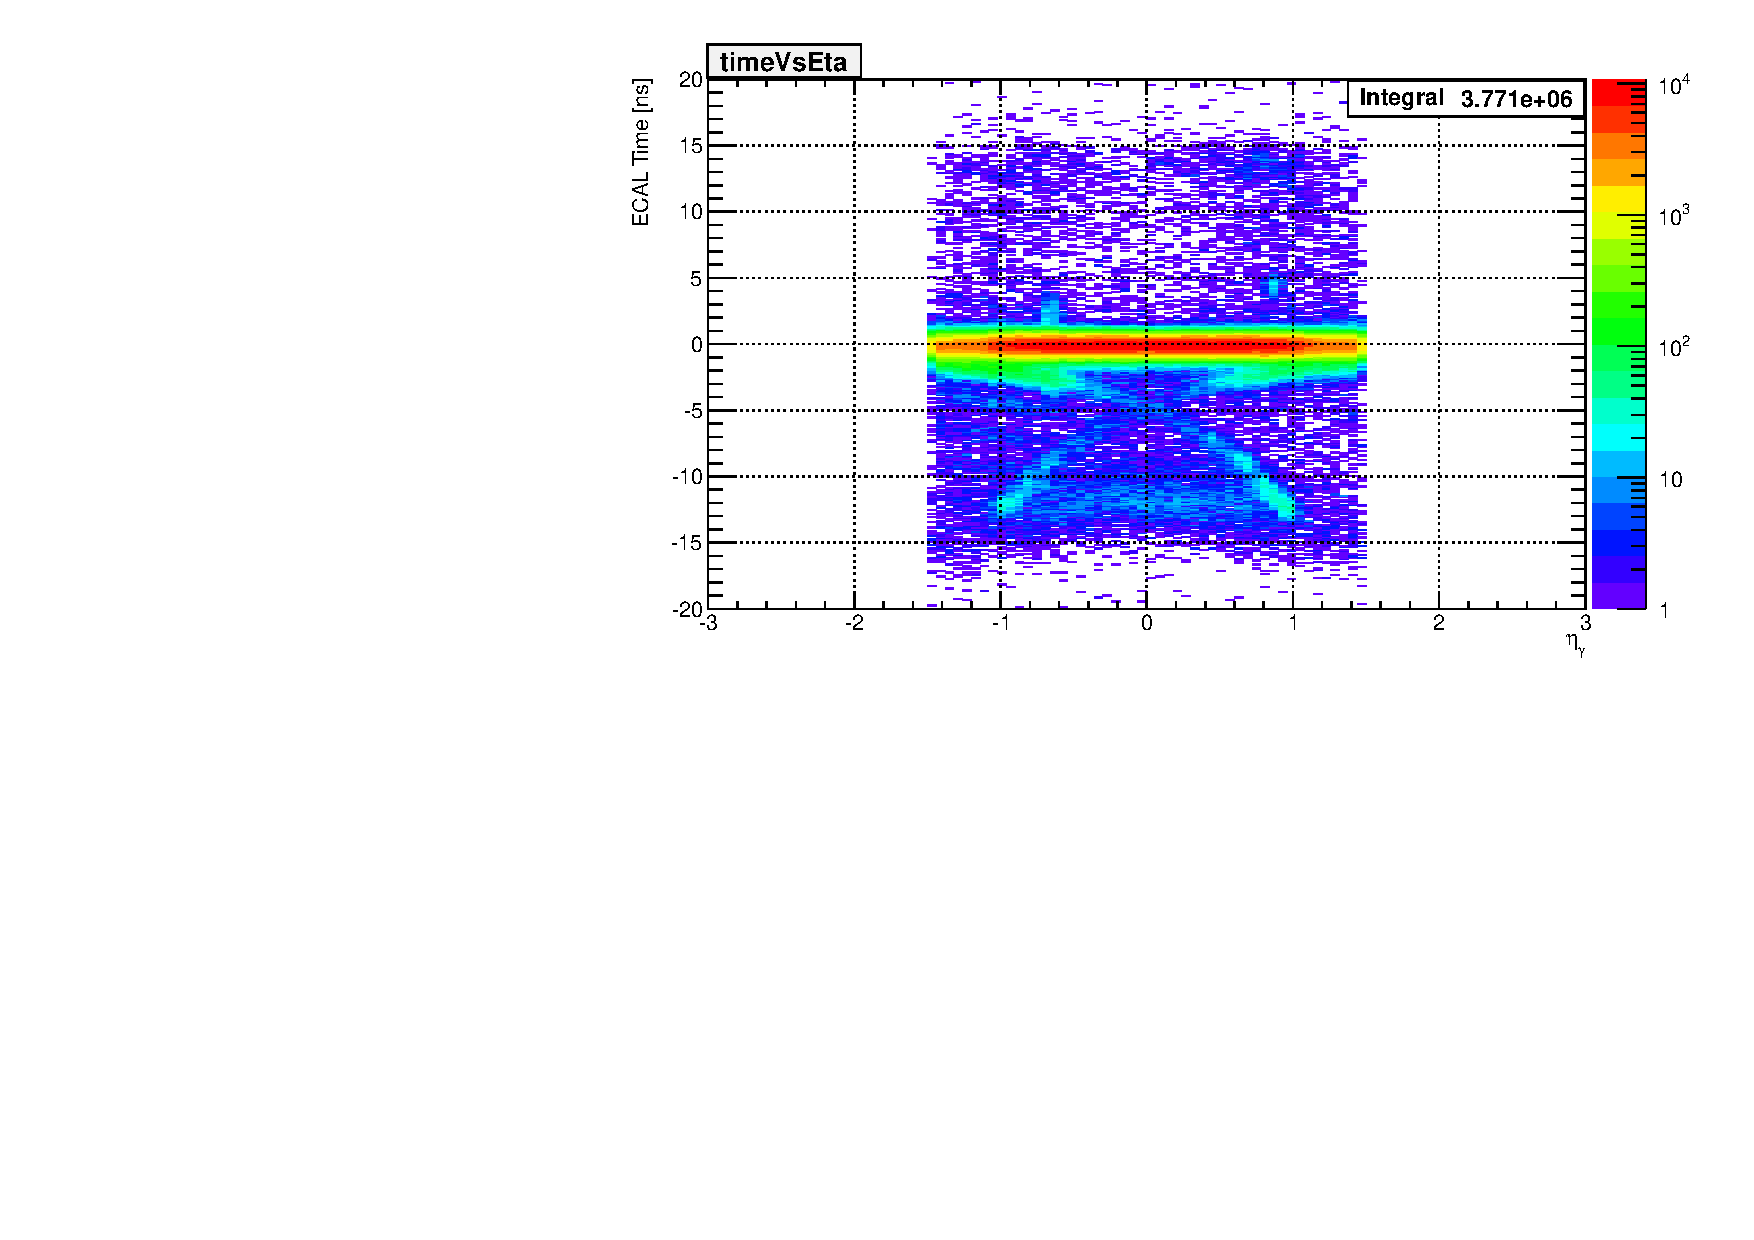
\includegraphics[height=0.340\textwidth, width=0.5\textwidth]{THESISPLOTS/SinglePhotonDataSet-TimeVsEtaEB.pdf}
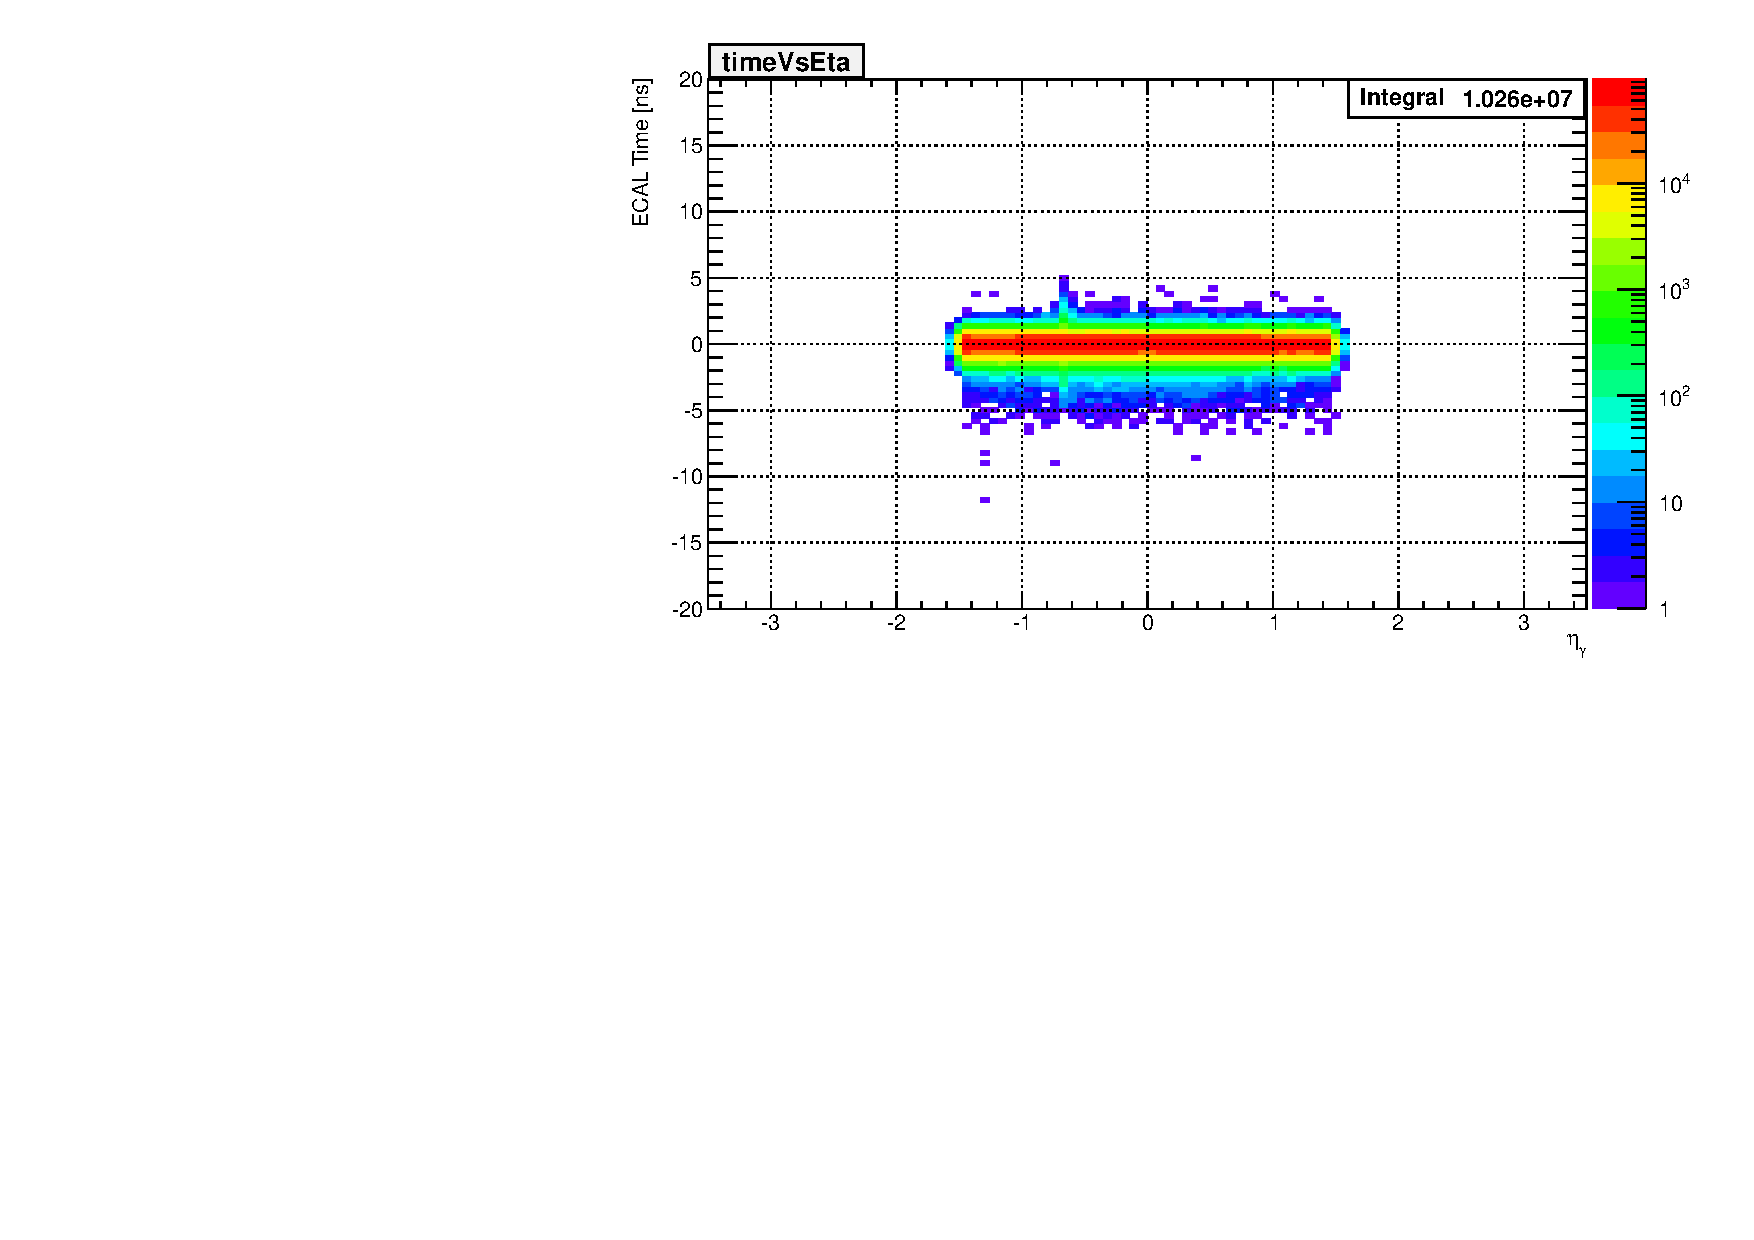
\includegraphics[height=0.340\textwidth, width=0.5\textwidth]
{THESISPLOTS/ZCandidates_TimeVsEta.pdf}}
\mbox{
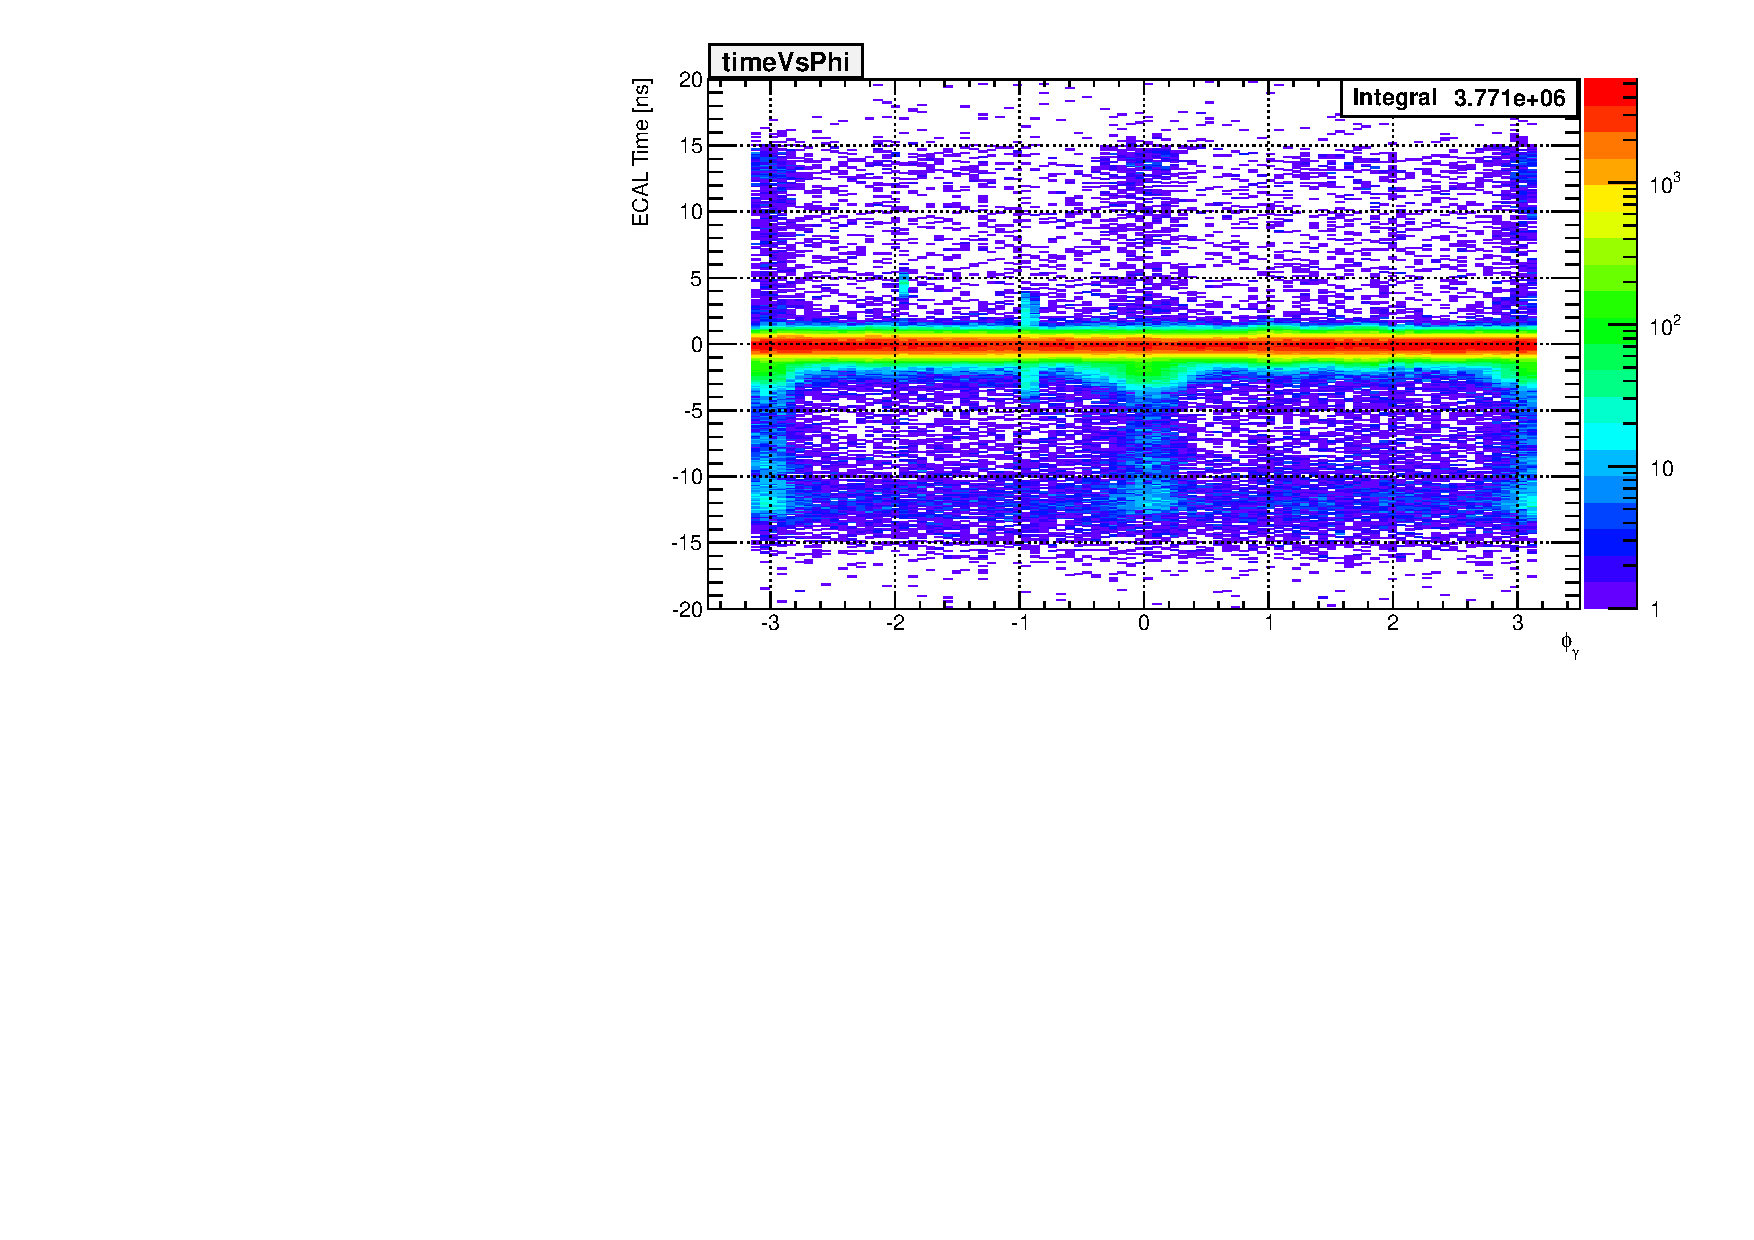
\includegraphics[height=0.340\textwidth, width=0.5\textwidth]{THESISPLOTS/SinglePhotonDataSet-TimeVsPhiEB.pdf}
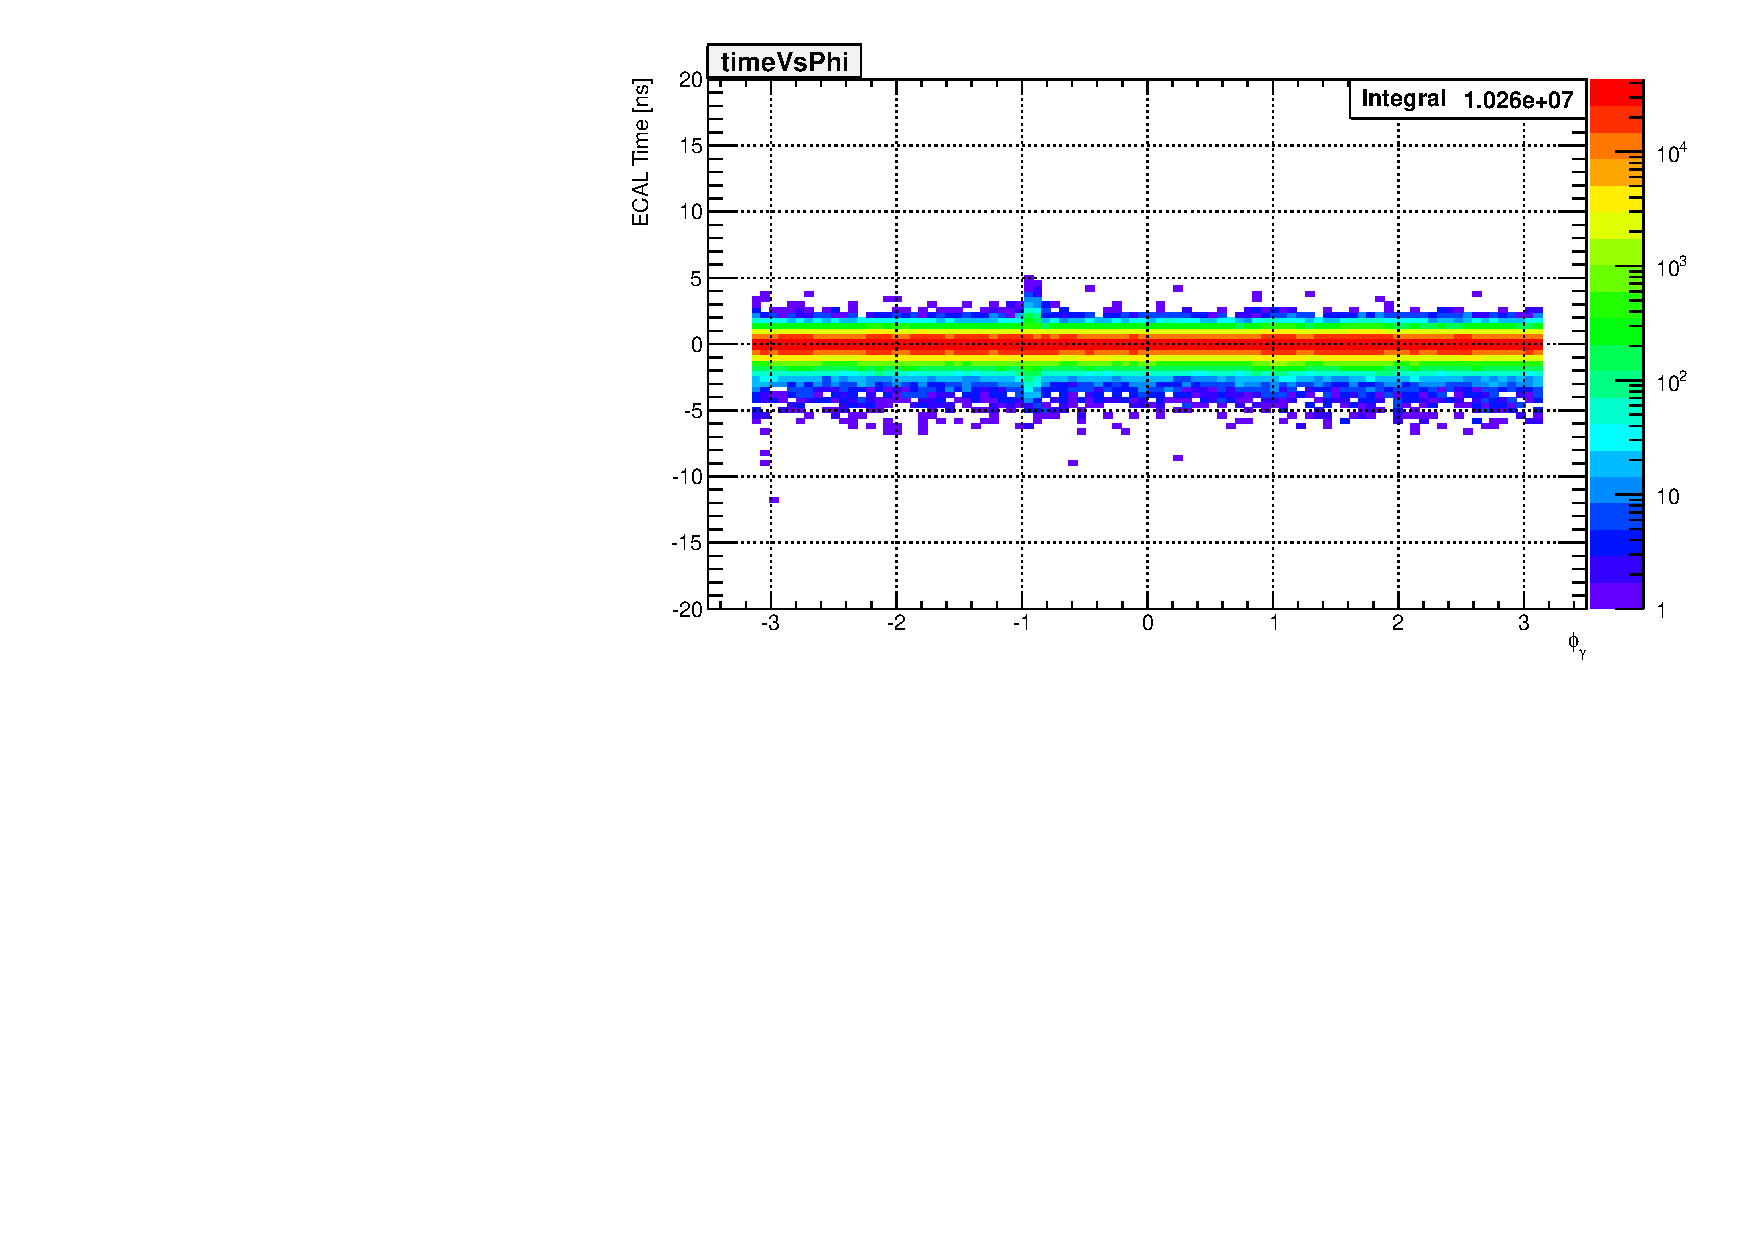
\includegraphics[height=0.340\textwidth, width=0.5\textwidth]{THESISPLOTS/ZCandidates_TimeVsPhi.pdf}}
\captionof{figure}{ECAL time, $t$ Vs $\eta$(top) and $t$ Vs $\phi$~(bottom) for photons from \texttt{SinglePhoton} dataset~(left) compared to electron candidates from the \texttt{DoubleElectron} dataset~(right). All photons or electron candidates are in barrel subdetector. Most of the photons with $\phi = 0, \pm \pi$ are halo photons which are not observed in the $\PZ$ boson candidate sample.}
\label{fig:Elec}
\end{center}
\end{minipage}

\vspace{5mm}
The di-electron mass(left) and electron arrival time(left) for signal~(blue) and background~(red) events is shown in Figure \ref{fig:Zmass}. The out-of-time background contribution to the \PZ event sample is estimated using a \textit{sideband subtraction method} described as follows:
\begin{itemize}
\item we fit the di-electron candidate mass distribution of the background control sample with a polynomial function(see top plots of Figure  \ref{fig:collZ}) to extract the background template.
\item using the background template, we obtain a scale factor $$\displaystyle{\mbox{Scale Factor} = \frac{N}{M_{1} + M_{2}}}$$~(see bottom plot of Figure \ref{fig:collZ}) which is use to determine the correct contribution of the background events to the the signal event sample.
\item After scaling the background control sample electron arrival ECAL time distribution~(red distribution of right plot in Figure \ref{fig:Zmass}) using the extracted scale factor and subtracting the scaled sideband control sample electron ECAL time distribution from the signal sample  electron ECAL time distribution~(blue distribution of right plot in Figure \ref{fig:Zmass}), the resulting distributions shown in Figure \ref{fig:Ztime} gives an estimate for out-of-time candidate events from collision.
\item The ratio of the total number of events with the electron ECAL time $t > 3$~ns to those with electron ECAL time, $|t| < 2$~ns, \ie $ N_{t > 3~ns}/ N_{|t| < 2.0~ns}$, gives an estimated fraction of out-of-time background events from collision. 
\end{itemize}  

\vspace{5mm}
\begin{minipage}{0.90\linewidth} 
\begin{center}
\mbox{
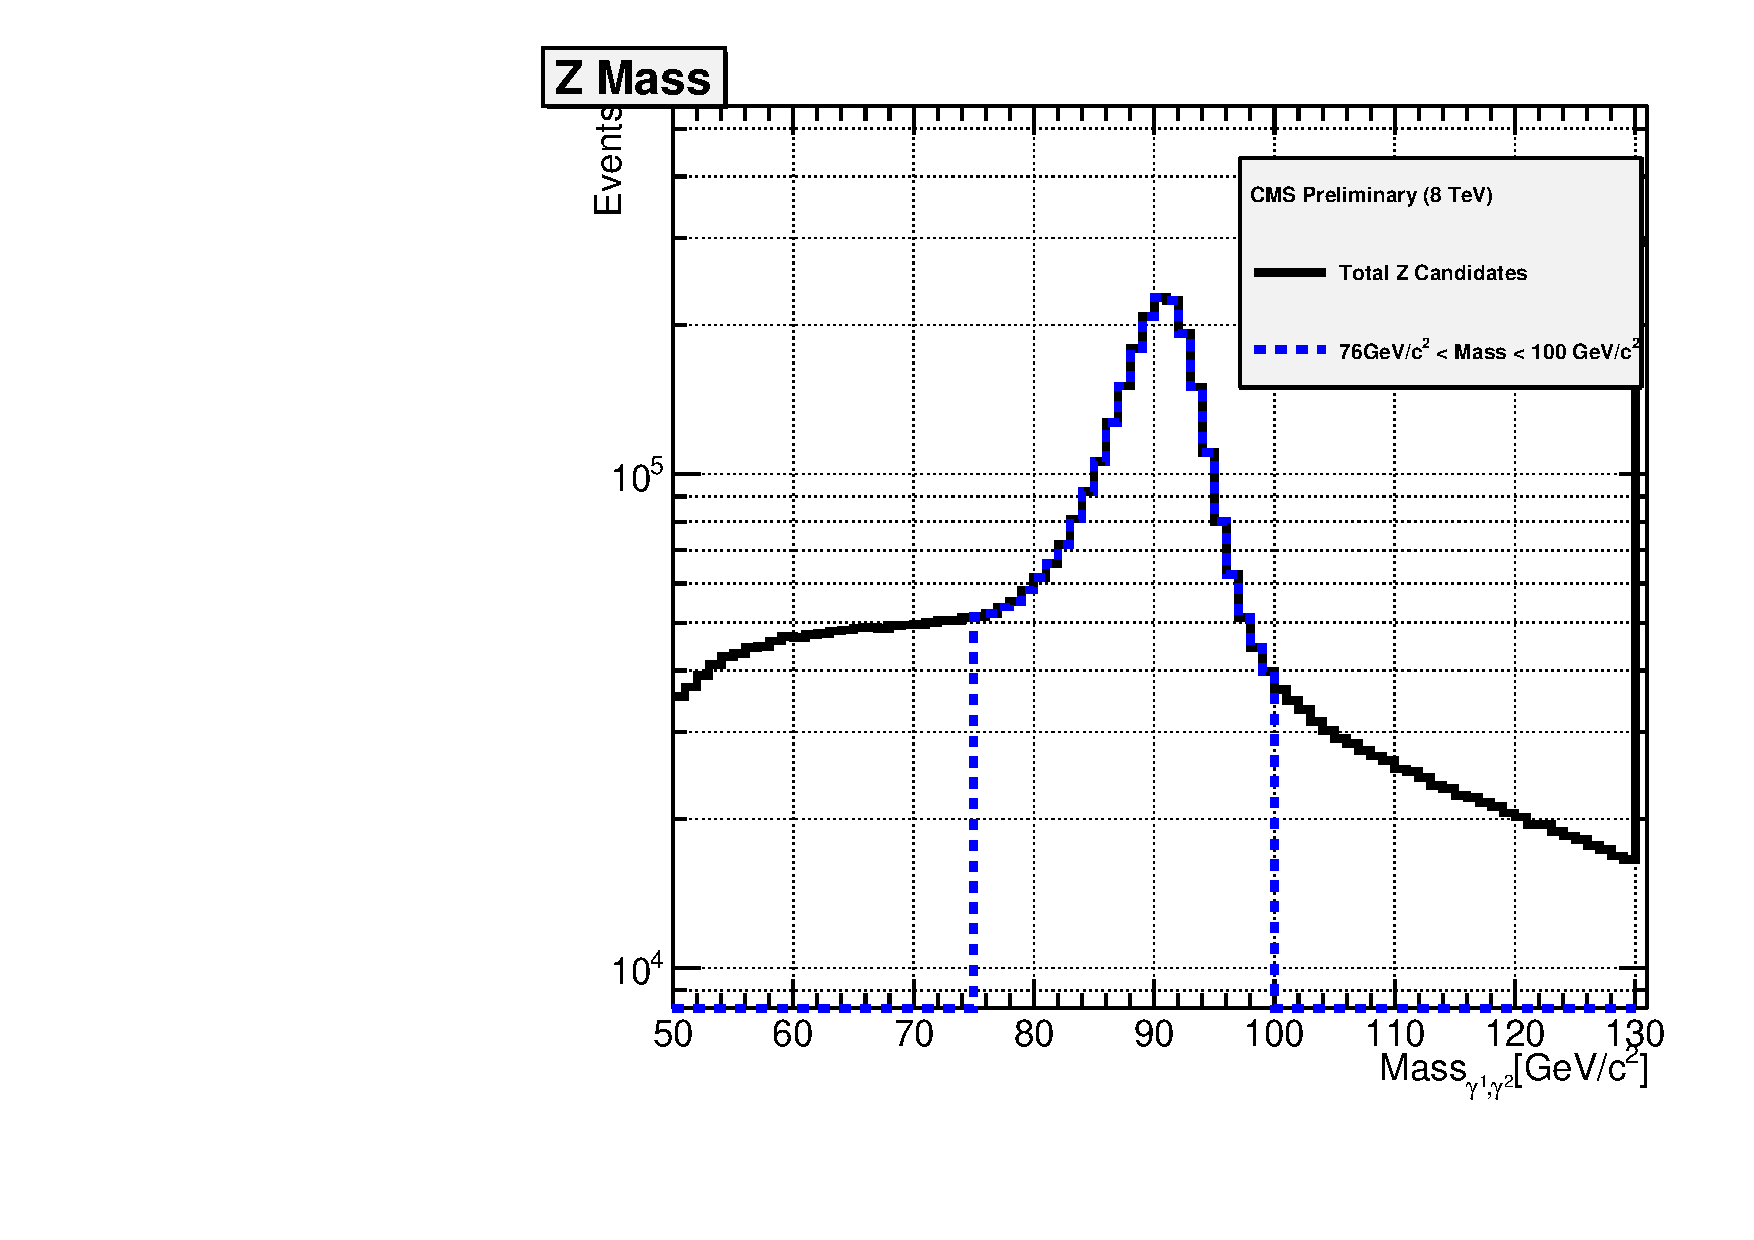
\includegraphics[height=0.55\textwidth, width=0.5\textwidth]{THESISPLOTS/Z-CandidateOverLay-SignalMass.pdf}
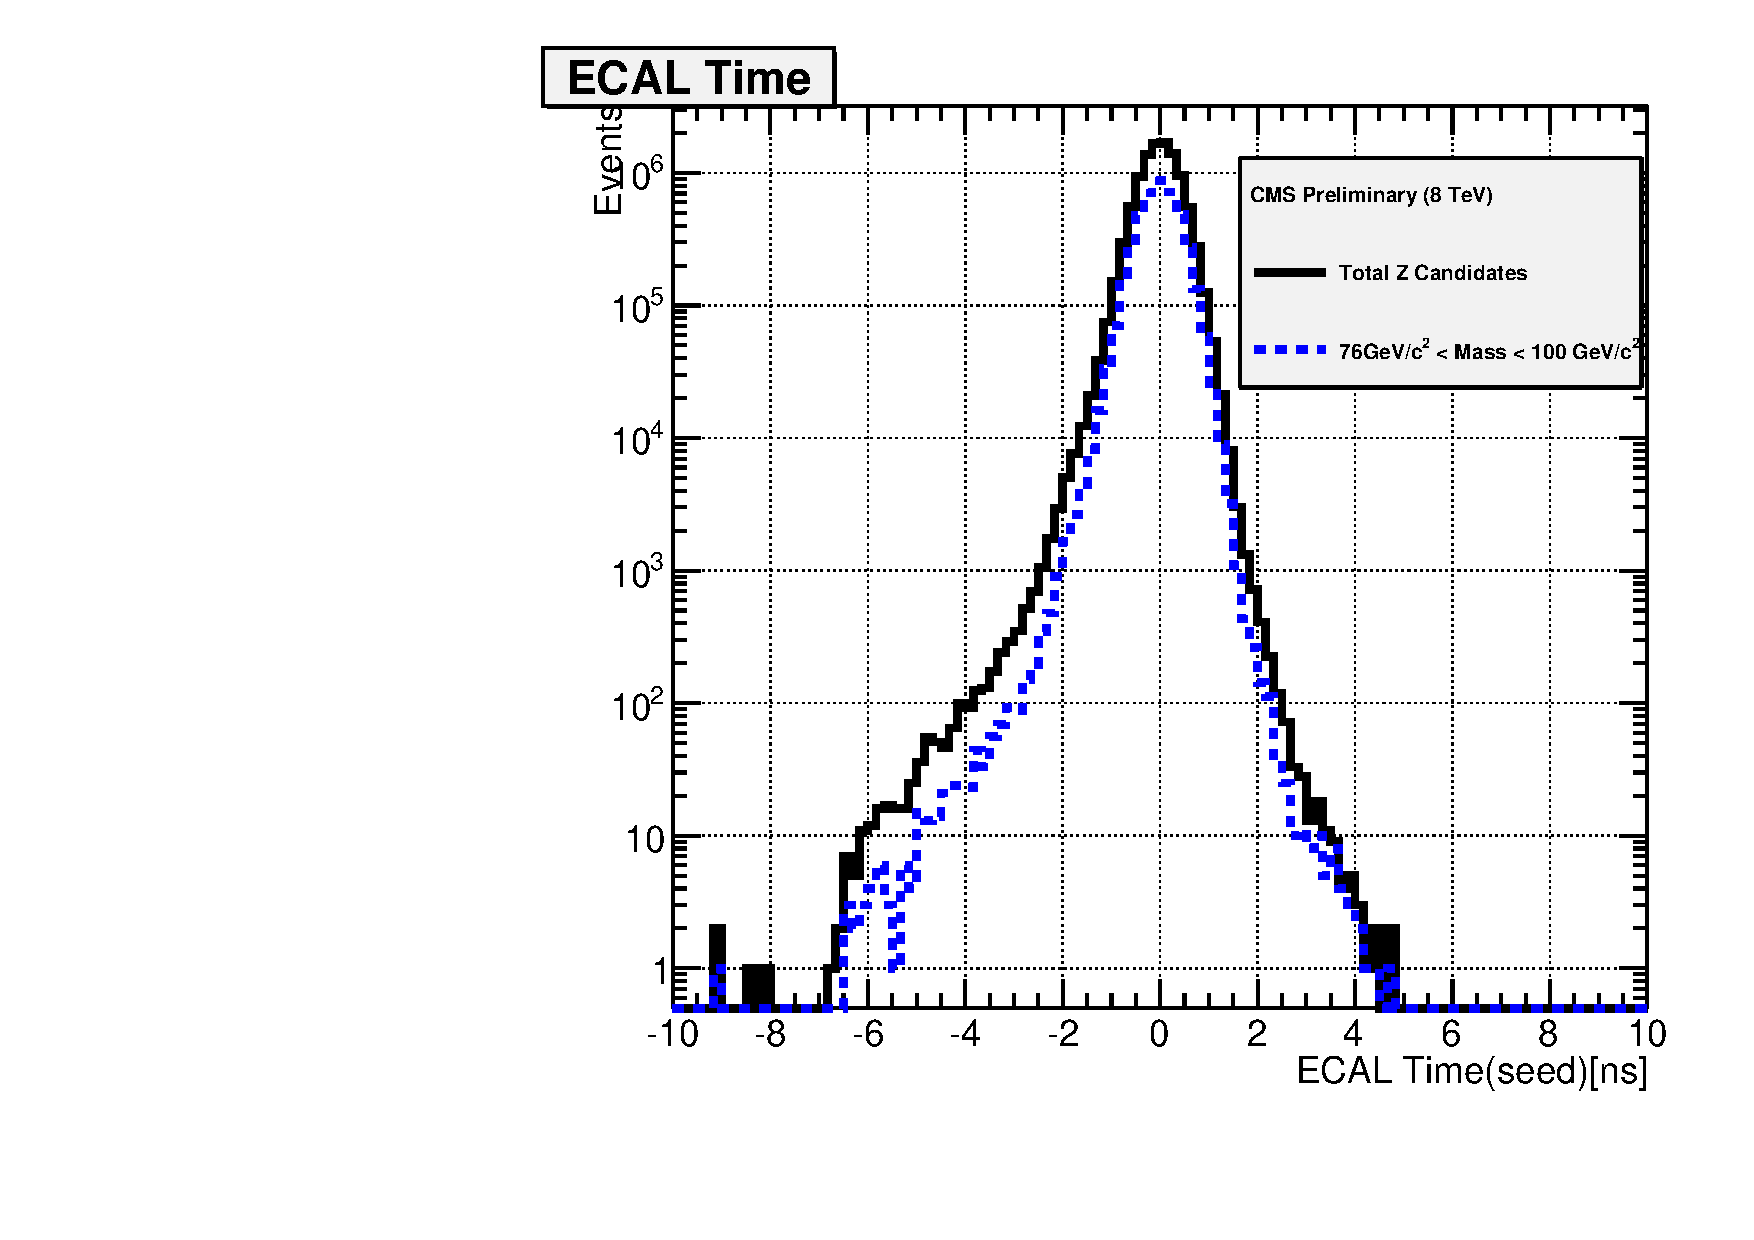
\includegraphics[height=0.55\textwidth, width=0.5\textwidth]{THESISPLOTS/Z-CandidateOverLay-SignalTime.pdf}}
\mbox{
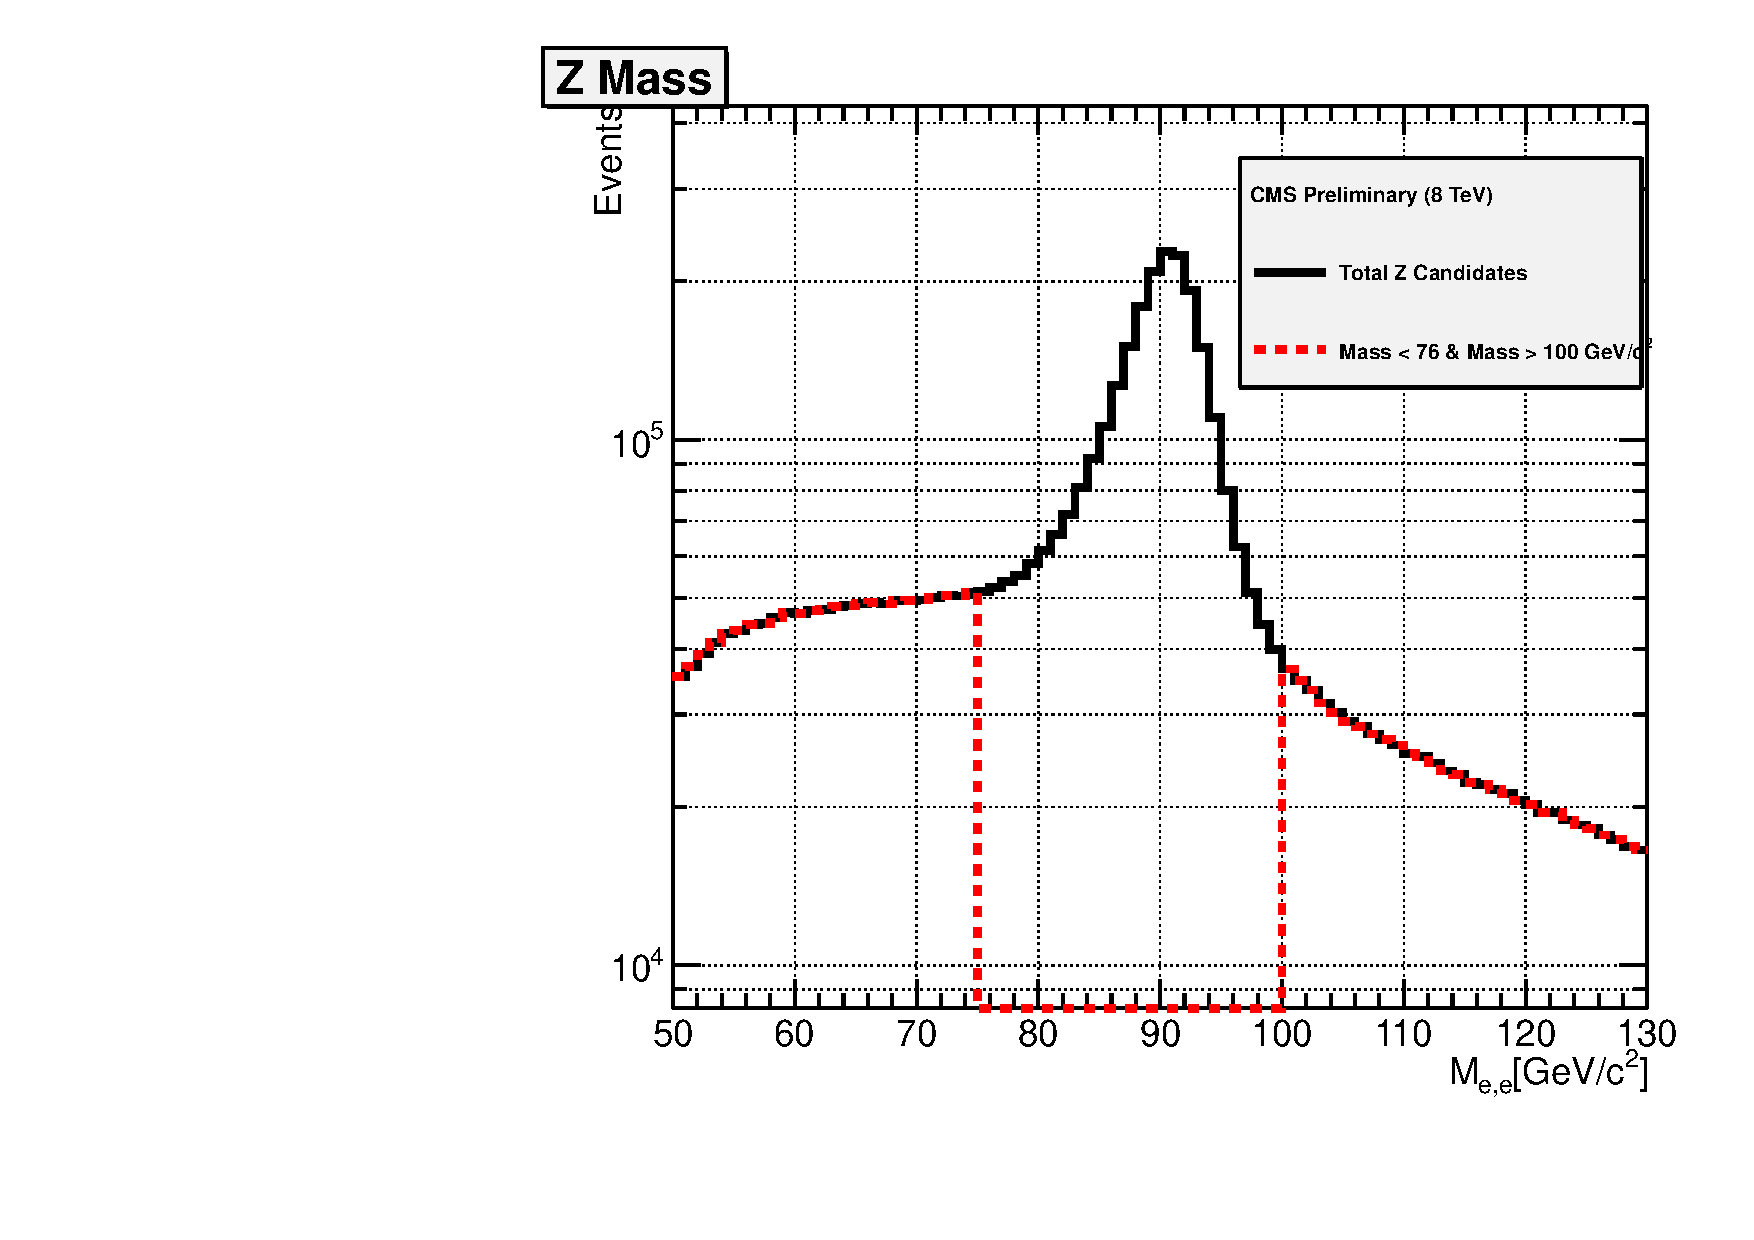
\includegraphics[height=0.55\textwidth, width=0.5\textwidth]{THESISPLOTS/Z-CandidateOverLay-BackgroundMass.pdf}
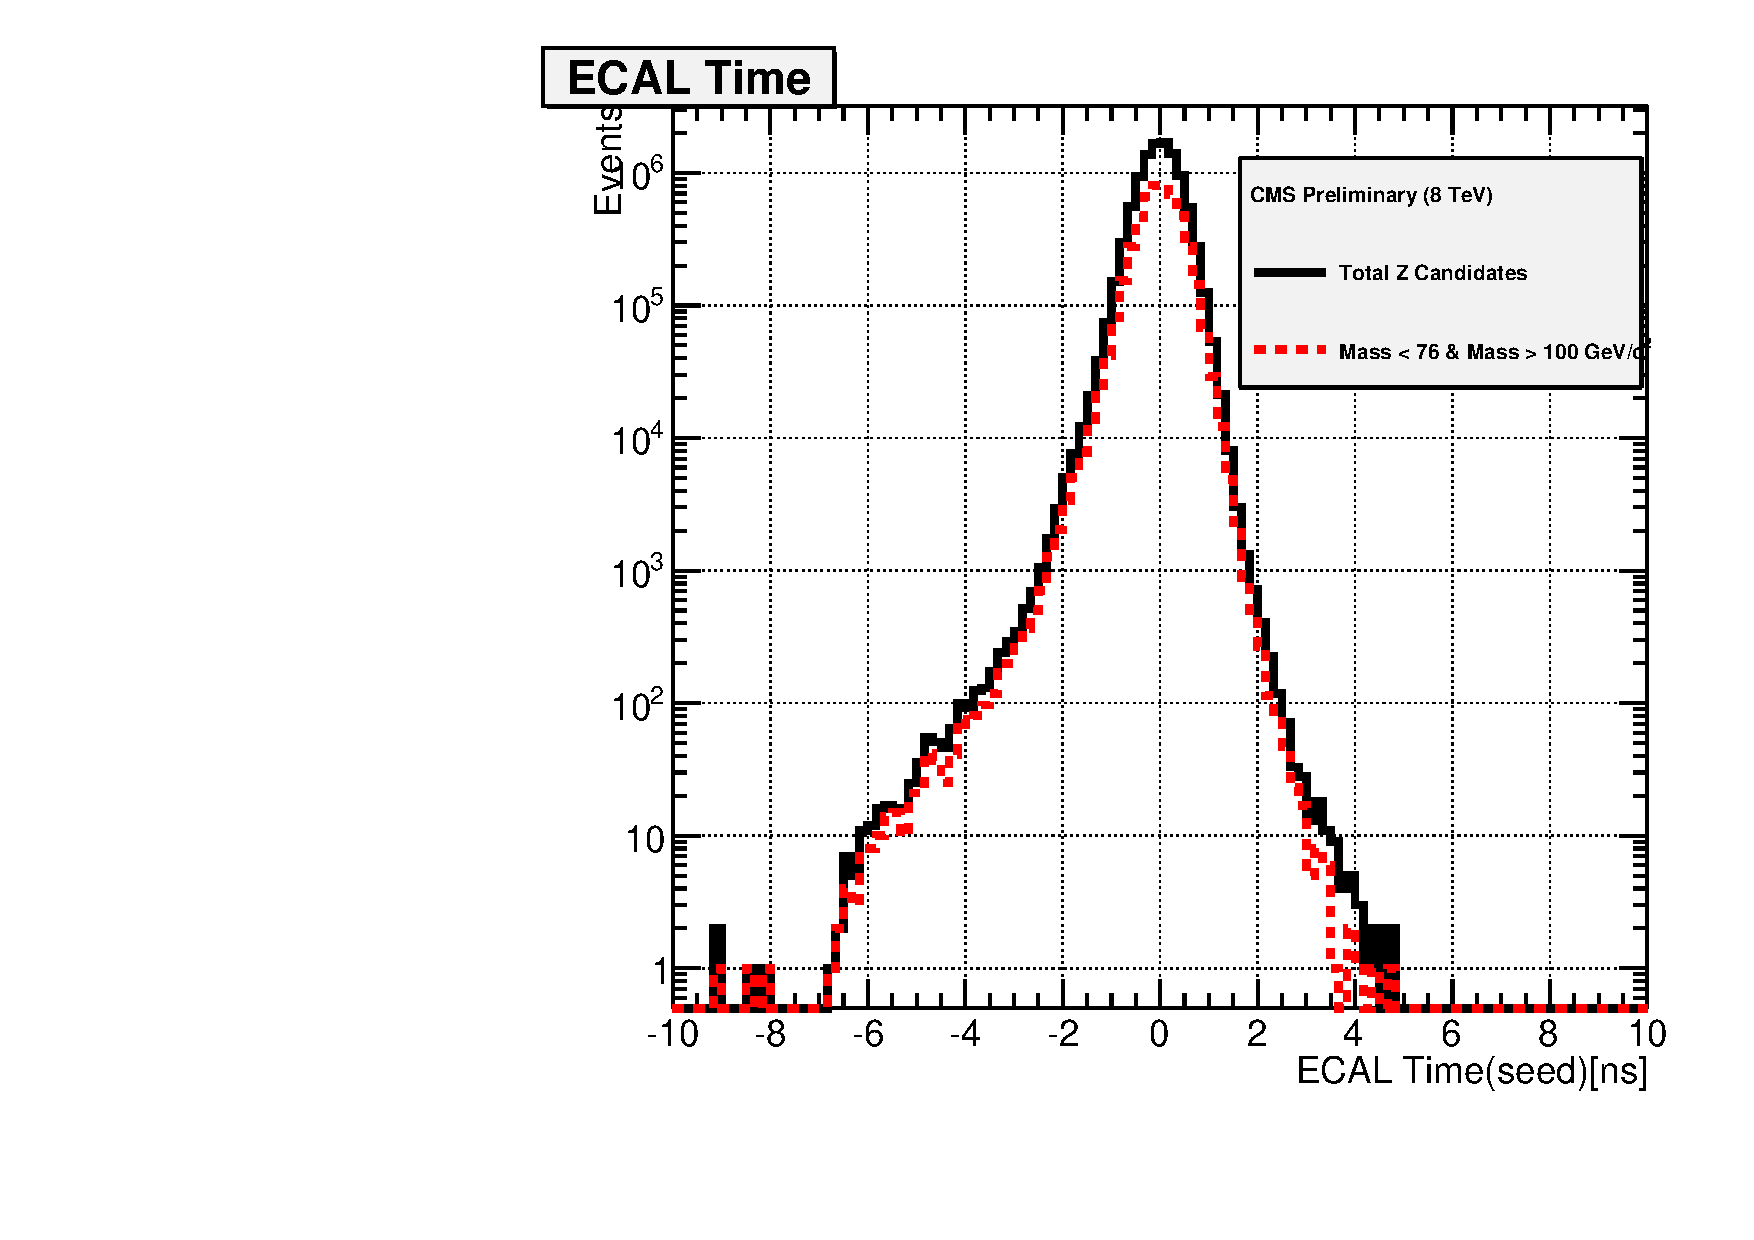
\includegraphics[height=0.55\textwidth, width=0.5\textwidth]{/home/tensr/Documents/TEN-HEP-PHD-THESIS/PHD_THESIS/PHD/THESISPLOTS/Z-CandidateOverLay-BackgroundTime.pdf}}
\captionof{figure}{Di-electron candidate mass distribution~(left) and the time~(right) of the two electrons for the signal \textcolor{blue}{$76 < m_{\EE} < 100$}\GeVcc $\PZ$ boson sample and for Control Samples~(\textcolor{red}{$50 < m_{\EE} < 76$}\GeVcc and \textcolor{red}{$ 100 < m_{\EE} < 130$}\GeVcc). Candidates events are from the \texttt{DoubleElectron} data sample.}
\label{fig:Zmass}
\end{center}
\end{minipage}

\vspace{5mm}
\begin{minipage}{0.90\linewidth} 
\begin{center}
\mbox{
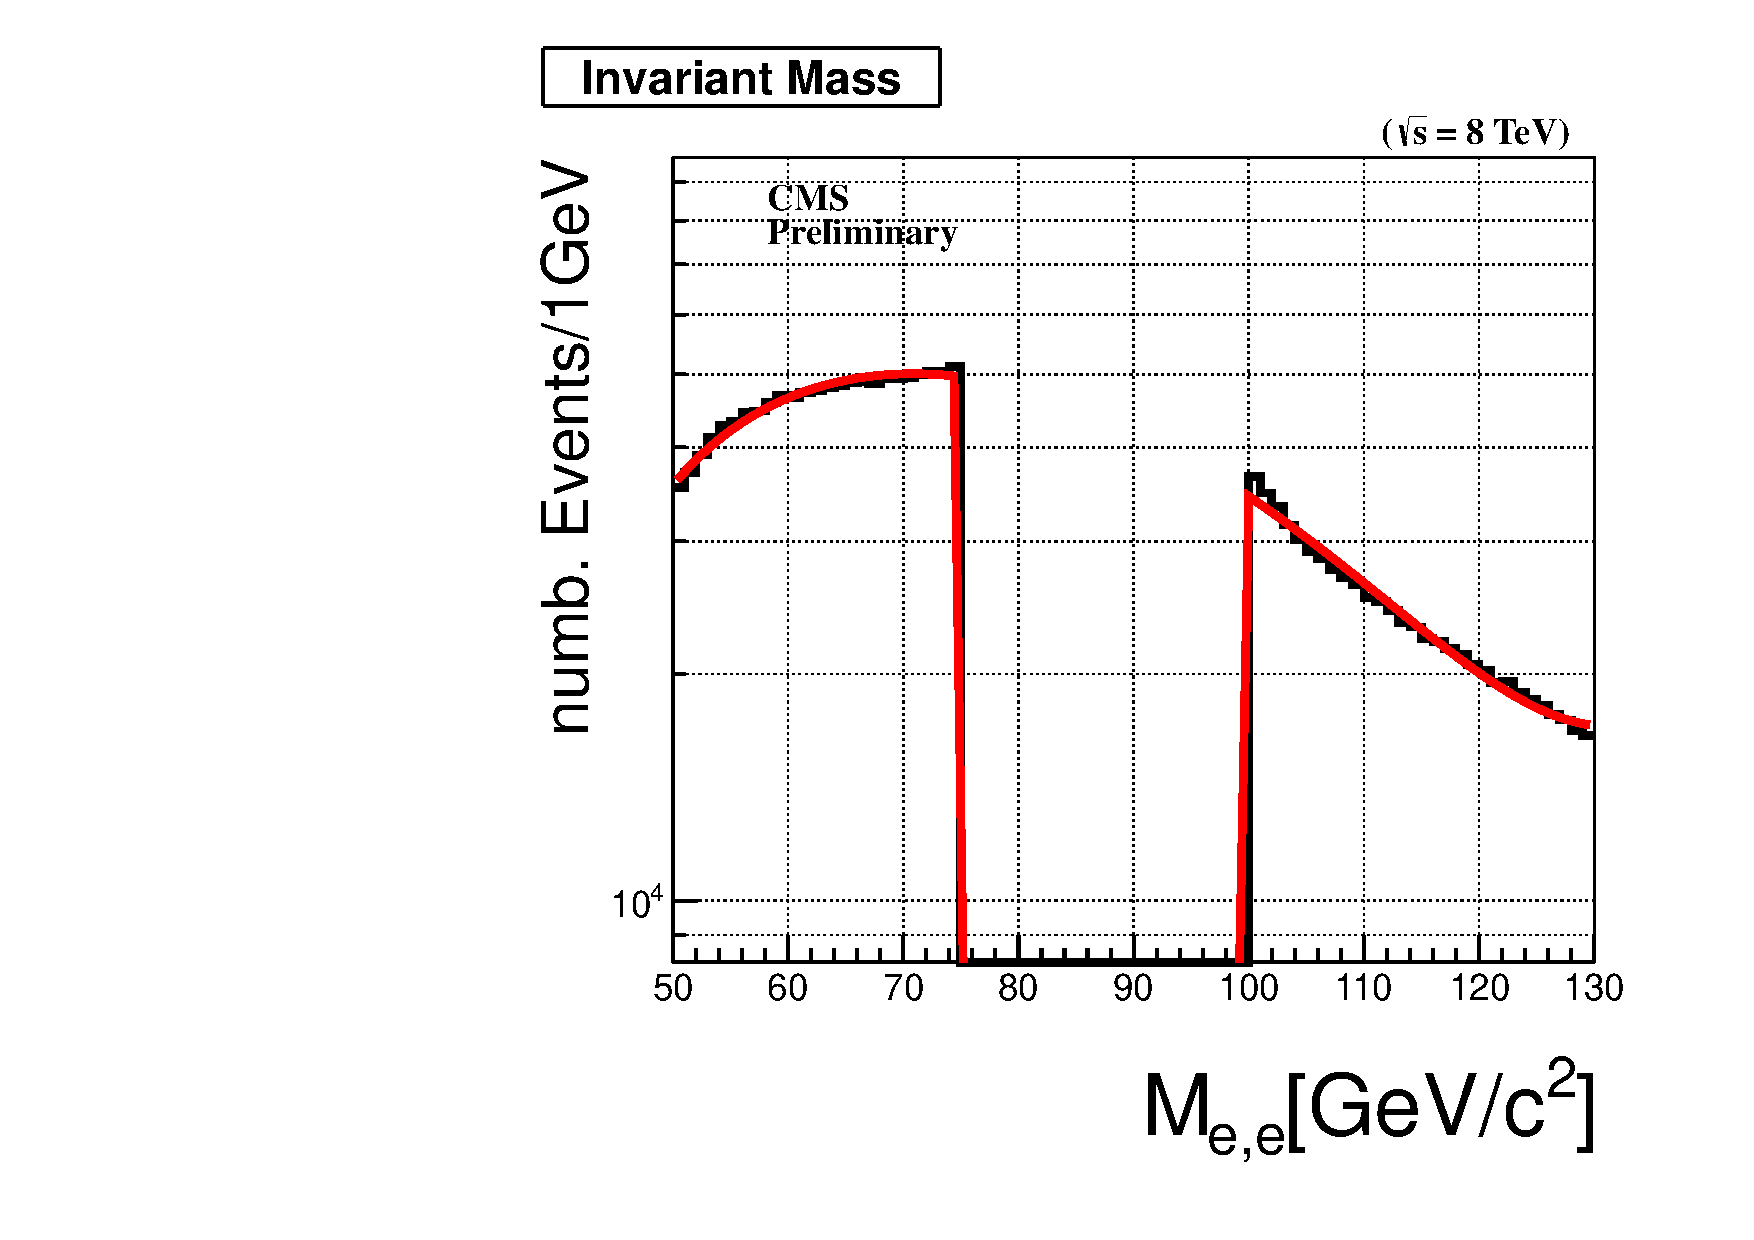
\includegraphics[height=0.50\textwidth, width=0.5\textwidth]{THESISPLOTS/Uncleaned-di-Photon-ZMass-Fit-DoubleElectron-Run2012A.pdf}
\includegraphics[height=0.50\textwidth, width=0.5\textwidth]{THESISPLOTS/Background_In_ZMass-From-Di-Photon.pdf}}
\mbox{
\includegraphics[height=0.55\textwidth, width=0.8\textwidth]{THESISPLOTS/ZBackground_SF.png}
%\includegraphics[height=6cm, width=0.5\textwidth]{THESISPLOTS/CMS_Slice.png}
}
\captionof{figure}{\textit{Top}: Polynomial fit~(red \& blue lines) of the di-electron invariant mass of candidate \PZ events for the sideband control sample~(left) only and all \PZ events~(right). \textit{Bottom:} Fitting the sideband CS to extract the scale factor use for estimating sideband event contribution in signal sample.}
\label{fig:collZ}
\end{center}
\end{minipage}
%%%%%$$$$$
\vspace{5mm}
  The estimated ratio for out-of-time events to in-time collision events for the final time distribution of signal electron candidates after the normalized sideband subtraction, shown in Figure \ref{fig:Ztime} is about, $N_{t > 3~ns}/ N_{|t| < 2.0~ns} = 1.29 ^{+0.374}_{-0.325} \times 10^{-5}$.
In order to get the estimated number of background events of the neutralino decay signal from collisions in the control sample \textsf{D}, $N^{col}_{D}$, we multiply this ratio to the total number of in-time events from the neutralino decay signal event selections which is $28282$. This gives $N^{col}_{D} = 0.366^{+0.106}_{-0.092}$ events. Comparing this to the value obtained with the \textsf{ABCD} method, which is $\frac{28283}{1446522} = 0.0391^{+0.039}_{-0.047}$, we find that numbers from thw two methods of estimating the number of collision background events are not exactly equal. We cannot interpret this inequality between both methods of estimating the number of background events from collision. On the contrary, the fact that this ratio $N_{t > 3~ns}/ N_{|t| < 2.0~ns}$ is very small confirms our speculation that indeed the contribution of collision events with out-of-time photons to our background estimation is almost negligible~(less than a single event) such that the uncertainties on the ratio of out-of-time to in-time events used in our \textsf{ABCD} collision background estimation is irrelevant.  It is also important to not that, we have not applied any \MET selection requirements in selecting our \PZ candidate events. A simple cut, $\MET > 60$\GeV could further reduce this ratio to an even smaller number observed in our background estimation.
  
\vspace{5mm}
\begin{minipage}{0.90\linewidth} 
\begin{center}
%\mbox{
\includegraphics[height=0.55\textwidth, width=0.7\textwidth]{THESISPLOTS/Seed-Time-From-Uncleaned-di-photon-Mass-Fit-DoubleElectron-Run2012A.pdf}
%\includegraphics[scale=0.2]{THESISPLOTS/CMS_Slice.png}
\captionof{figure}{ECAL time distribution of genuine $\PZ$ bosons after background contribution is subtracted.}
\label{fig:Ztime}
\end{center}
\end{minipage}


\section{Systematic Studies}
The event selection requirements include a photon \pt greater than 80\GeVc, a jet \pt greater than 35\GeVc and missing energy greater than 60\GeV. We expect this same selections applied to our MC signal event sample to lead to good event selection efficiency. Therefore, any difference in the photon and jet \pt and missing transverse energy between MC and data will lead to systematic uncertainties in our event selection efficiency. We anticipate these uncertainties to come from quantities like jet energy scale~(JES), jet energy resolution~(JER), electron-photon energy scale, instrumentation related and missed or unclustered energy deposits in missing transverse energy reconstruction, photon ECAL arrival time bias and ECAL time resolution. In summary, the different sources of uncertainties considered in this analysis is presented in Table \ref{tab:SYST}. These uncertainties are obtain by varying the nominal values of each quantity while keeping the rest fixed by $1\sigma$ deviation and counting the number of events passing our event selection requirements. Our largest uncertainty is from ECAL timing bias on the absolute reference time(zero ns) of the ECAL timing to measured the photon arrival time. This has the larget impact on our analysis as our analysis is based on counting the number of events with photon ECAL time above $3$~ns. The next largest uncertainties are from unclustered energy deposits which affect missing energy scale and from jet energy scale and resolution.
\newline
The uncertainty on the photon energy scale in barrel was estimated to be 4.0\% and based on the final-state radiation~(FSR) in $Z\rightarrow \mu\mu\gamma$ events \cite{PES}.  The uncertainty on the \MET resolution uses a conservative estimate from \cite{METRES}. The uncertainty on the ECAL time resolution was obtained by comparing the peak in the photon ECAL time distribution of events from $\gamma +$ jet MC sample to events from data with photon ECAL time $|t| < 2$~ns. The difference is found to be of the order of 200~ps per event. A study using high \pt photons with energy beyond gain transitions has was also performed and this discrepancy was observed to be worse. 
The systematic uncertainty on luminosity measurement has the recommended value of $2.2$\% provided by CMS and LHC luminosity measurements while the uncertainty from pardon density functions~(PDF) is evaluated using the re-weighting technique which uses the Master Equation of CTEQ65 model set described in \cite{PDF}.
\par
Another important source of systematic is in the selection of the background control samples and our background estimation and individual systematic in the tagging and mistagging of non-collision background and estimating background contributions from collisions. We combined these separate uncertainty contributions into a single background estimation uncertainty referred here as our background estimation uncertain. 
However, since our background estimation is data-driven, most of the uncertainties arising due to systematic can be neglected~(less than 1\% impact) as the cancel out.
This is our largest source of uncertainty in our analysis which we estimate to vary it upward by 223\% and downward by 51\% as a statistical uncertainty in the \textsf{ABCD} background estimation method. The large background statistical uncertainty is due to very low event statistics. However, despite the large background estimation uncertainty, the signal selection uncertainties are the most significant uncertainties which impact our final results. These uncertainties are used as nuissance parameters in the calculation of the upper limit on observed signal cross-section~($\sigma_{UL}$).

\vspace{5mm}
\begin{minipage}{0.90\linewidth} 
\begin{center}
%\begin{table}[ht]
%\renewcommand\arraystretch{1.2}
\begin{tabular}{c c}
\toprule
\hline
\bfseries{Source} & \bfseries {Uncertainty(\%)}\\
\hline
\toprule
\texttt{ECAL absolute time }~(0.0~ns) & $<10.0$\% \\
\texttt{ECAL time resolution}~(0.5~ns) & $<5.0$\% \\
\texttt{Unclustered energy deposits} & $<9.0$\% \\
\texttt{Photon energy scale}  & $< 4.0$\% \\
\texttt{Jet energy scale}~(JES)  & $< 9.0$\% \\
\texttt{Jet energy resolution}~(JER) &$ <9.0$\% \\
\texttt{\MET resolution} & $ <2.8$\%  \\
\texttt{PDF uncertainty} & $< 1.70$\% \\
\hline
\toprule
\texttt{Background estimation uncertainty} &$51.0$\% to 223\% \\
\hline 
\texttt{Luminosity}~(4.5\%) & $< 2.2$\% \\
\hline
\bottomrule
\end{tabular}
\captionof{table}{Summary of systematic uncertainties for signal efficiency and background estimation in this analysis and applied to our final results.}
\label{tab:SYST}
%\end{table}
\end{center}
\end{minipage}


\section{Results}
After running our analysis on the SinglePhoton data samples requiring events with at least 2 jets, at least one photon with ECAL time  $ 3.0 < t_{\gamma} < 13.0$~ns, ${\ETslash}^{\gamma}\hspace{0.15cm} > 60$\GeV, and $\ETslash\hspace{0.15cm} > 60$\GeV, we observed a single event passing all our event selection requirements as a signal event. This event has one photon and two jets. The photon has a transverse momentum  of 224\GeVc and an ECAL time of 12.17~ns.
\newline
Our final expected number of background events estimated is $0.093^{+0.301}_{-0.047}$. This number was computed as
\begin{align*} 
 N_{B}^{col} &= \frac{28283}{605496} \times 3 = 0.140^{+0.108}_{-0.061} \\
 N_{D}^{col} &= \frac{28283}{605496} \times 2 = 0.093^{+0.093}_{-0.047} \\
 N_{D}^{Total} &= \left( \frac{1 - 0.14}{3}\times 0\right) +  0.093 = 0.093^{+0.301}_{-0.047}.
\end{align*}
using the event yields and background events vetoed presented in Table \ref{tab:RESULT}. 

\vspace{5mm}
\begin{minipage}{0.90\linewidth} 
\begin{center}
\begin{tabular}{c| c| c| c| c }
\toprule
 \hline
\bfseries{Control Sample} & Yield & Beam Halo & Cosmic & Spike \\
\hline
\toprule
\textsf{D} & 1 & 0 & 0 & 0 \\
\textsc{C} & 0 & 2 & 1& 0  \\
\textsf{B} & 1 & 1&  1 &  1\\
\textsf{A} & 3 & 6 & 0 & 0\\
\hline\hline
\textsf{$A^{\prime}$}& 2 & 0 & 0 & 0\\ 
\textsf{$C^{\prime}$}& 4 & 0 & 0 & 0\\  
\textsf{$I$} & 28283 & -& - & -\\    
\textsf{$I^{\prime}$}&  669013 & - & - & \\       
\hline
\bottomrule
\end{tabular}
\captionof{table}{Event yields used in our final background estimation for signal candidate events with at least a single photon and at least 2 jets, ${\ETslash}^{\gamma}\hspace{0.15cm} > 60$\GeV, and $\ETslash\hspace{0.15cm} > 60$\GeV. }
\label{tab:RESULT} 
\end{center}
\end{minipage}

\vspace{5mm} 
With no significant excess over expected number of background events, we find upper limits on the number of event counts at 95\% confidence limit using the statistical CLs limit finding method.
%\paragraph*{}\mbox{}\\
%\begin{minipage}{\linewidth} 
%\begin{center}
%\centering
%%\begin{tabular}{|c| c| c|}
%%%\mbox{Fake Rate }
%%\toprule
%%\hline
%%\bfseries{Non-Collision} & $\mathbf{{\ETslash}^{\gamma}\hspace{0.15cm}} < 60$\GeV & $\mathbf{{\ETslash}^{\gamma}\hspace{0.15cm}} > 60$\GeV \\
%%\hline
%% $3.0 < t_{\gamma} < 13.0$~ns & \textsf{$C$}($0$) & ~\textsf{$D$}(\textcolor{blue}{$1$}) \\
%% $-10.0 < t_{\gamma} < -3.0$~ns & \textsf{$A$}($5$) & ~\textsf{$B$}($1$) \\
%%\hline \hline
%%\bfseries{Collision} & $\mathbf{\ETslash\hspace{0.15cm}} < 60$\GeV & $\mathbf{\ETslash\hspace{0.15cm}} > 60$\GeV \\
%%\hline 
%% $3.0 < t_{\gamma} < 13.0$~ns & \textsf{$D^{\prime}$}($5$) & ~\textsf{D} \textcolor{red}{$0.0888 ^{+0.1869}_{-0.0444}$} \\
%% $-2.0 < t_{\gamma} < 2.0$~ns & \textsf{$F^{\prime}$}($657663$) & ~\textsf{$F$}($30242$) \\
%% $-10.0 < t_{\gamma} < -3.0$~ns & \textsf{$B^{\prime}$}($1$) & ~\textsf{$B$} $0.23 ^{+0.092}_{-0.118}$) \\
%%\hline
%%\bottomrule
%%\end{tabular}
%%\captionof{table}{Result of observed events and estimated background from signal sample, events with at least $2$-jets. Numbers in bracket represent our observed number of events while numbers not is bracket are our expected number of background events estimated using \textsf{ABCD} method.}
%%\label{tab:RF} 
%%\end{center}
%%\end{minipage}
%%\paragraph*{}\mbox{}\\
\label{Search_Analysis_chapter}